\chapter{Ergebnisse}
    Um verschiedene antiferromagnetische Oberflächen zu untersuchen wurden Nickeloxidfilme in dem Versuchsaufbau aus \autoref{sec:Versuchsaufbau} vorbereitet und vermessen.
    Dabei betrug die Photonenenergie immer \SI{21.22}{\electronvolt} und die Probe befand sich bei Raumtemperatur.
    Ergebnisse dieser Präparation finden sich in \autoref{sec:Prep_NiO}.
    Das Eisenmonooxid wurde an der NanoESCA Beamline am Synchrotron Elettra in Trieste präpariert und charakterisiert \footnote{Näheres zu diesem Versuchsaufbau und der Behandlung der Daten kann in~\cite{ma-DJ} gefunden werden.}.
    Die Details dieses Prozesses sind in \autoref{sec:Prep_FeO} zusammengefasst.
    Auf beide Substrate wurden Pentacen Moleküle aufgedampft und mittels der Beugung niederenergetischer Elektronen (\textit{low energy electron diffraction}, LEED), sowie der Photoemissionsorbitaltomographie betrachtet.
    DieErgebnisse sind in \autoref{sec:Ergeb} zusammendargestellt.
    Zur Analyse und Bearbeitung der Daten wurden IGOR Pro 8~\cite{IGOR} und Spot Plotter~\cite{SpotPlotter} verwendet. % und Inkscape~\cite{Inkscape} Anwendung.

    \section{Nickeloxid} \label{sec:Prep_NiO}
        \begin{figure}
            \centering
            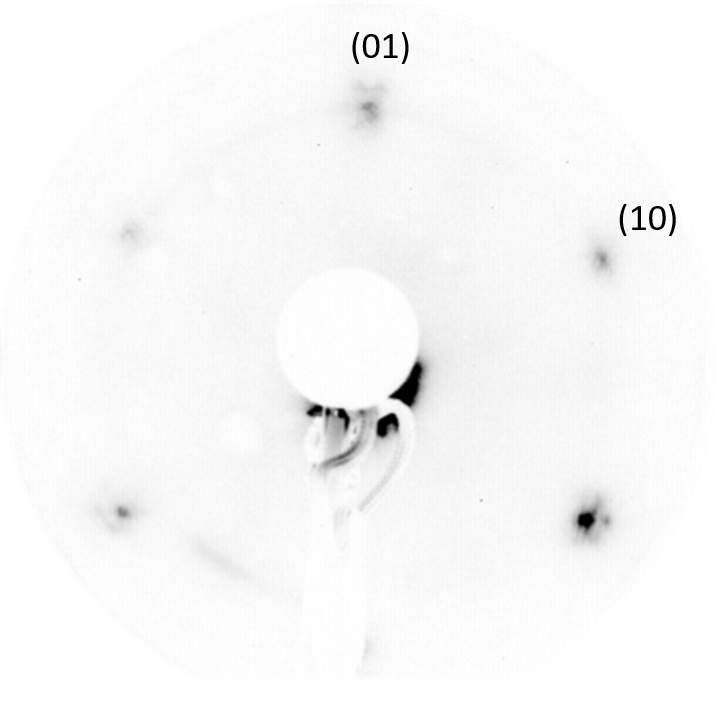
\includegraphics[height=5cm]{Au/2021_06_08_002_Au(111)_75eV_mod.png}            
            \caption{Das Beugungsbild der sauberen Gold (111)-Oberfläche bei einer Elektronenenergie von \SI{75}{\electronvolt}.}
            \label{fig:LEED_Au}
        \end{figure}
        Zur Präparation des antiferromagnetischen Nickeloxidfilms wird die Gold (111)-Oberfläche verwendet.
        Das Substrat wurde zunächste mehrere Male durch ioneninduziertes Zerstäuben und anschließendes Aufheizen auf \SI{500}{\celsius} gereinigt.
        Dies führt zu einer wohldefinierten, sauberen Oberfläche was sich auch anhand der scharfen Spots im LEED-Bild erkennen lässt (siehe \autoref{fig:LEED_Au}).
        Zudem sind auch die zusätzlichen Spots aufgrund der Fischgräten-Rekonstruktion sichtbar, welche sich um die Hauptspots herum verteilen.
        Die unterschiedlichen Intensitäten der einzelnen Reflexe rühren ebenfalls von der Rekonstruktion her~\cite{haag_epitaxial_2016}.

        \begin{figure}
            \centering
            \begin{subfigure}[t]{0.34\textwidth}
                \centering
                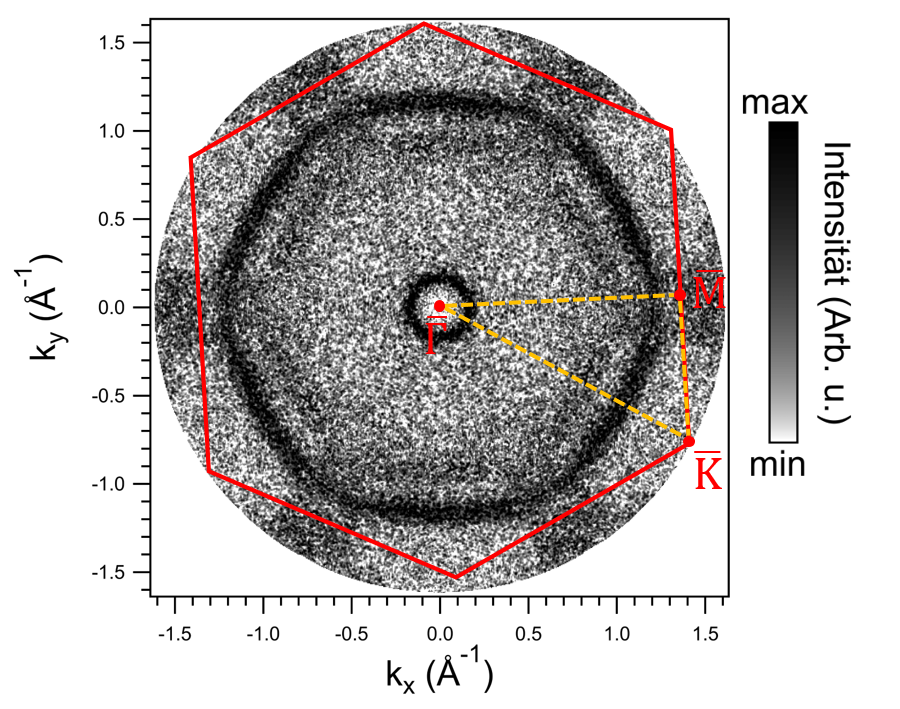
\includegraphics[height=3.74cm]{Au/BZ_Au_2.png}
                \subcaption{}
                \label{fig:BZ_Au}
            \end{subfigure}
            \begin{subfigure}[t]{0.62\textwidth}
                \centering
                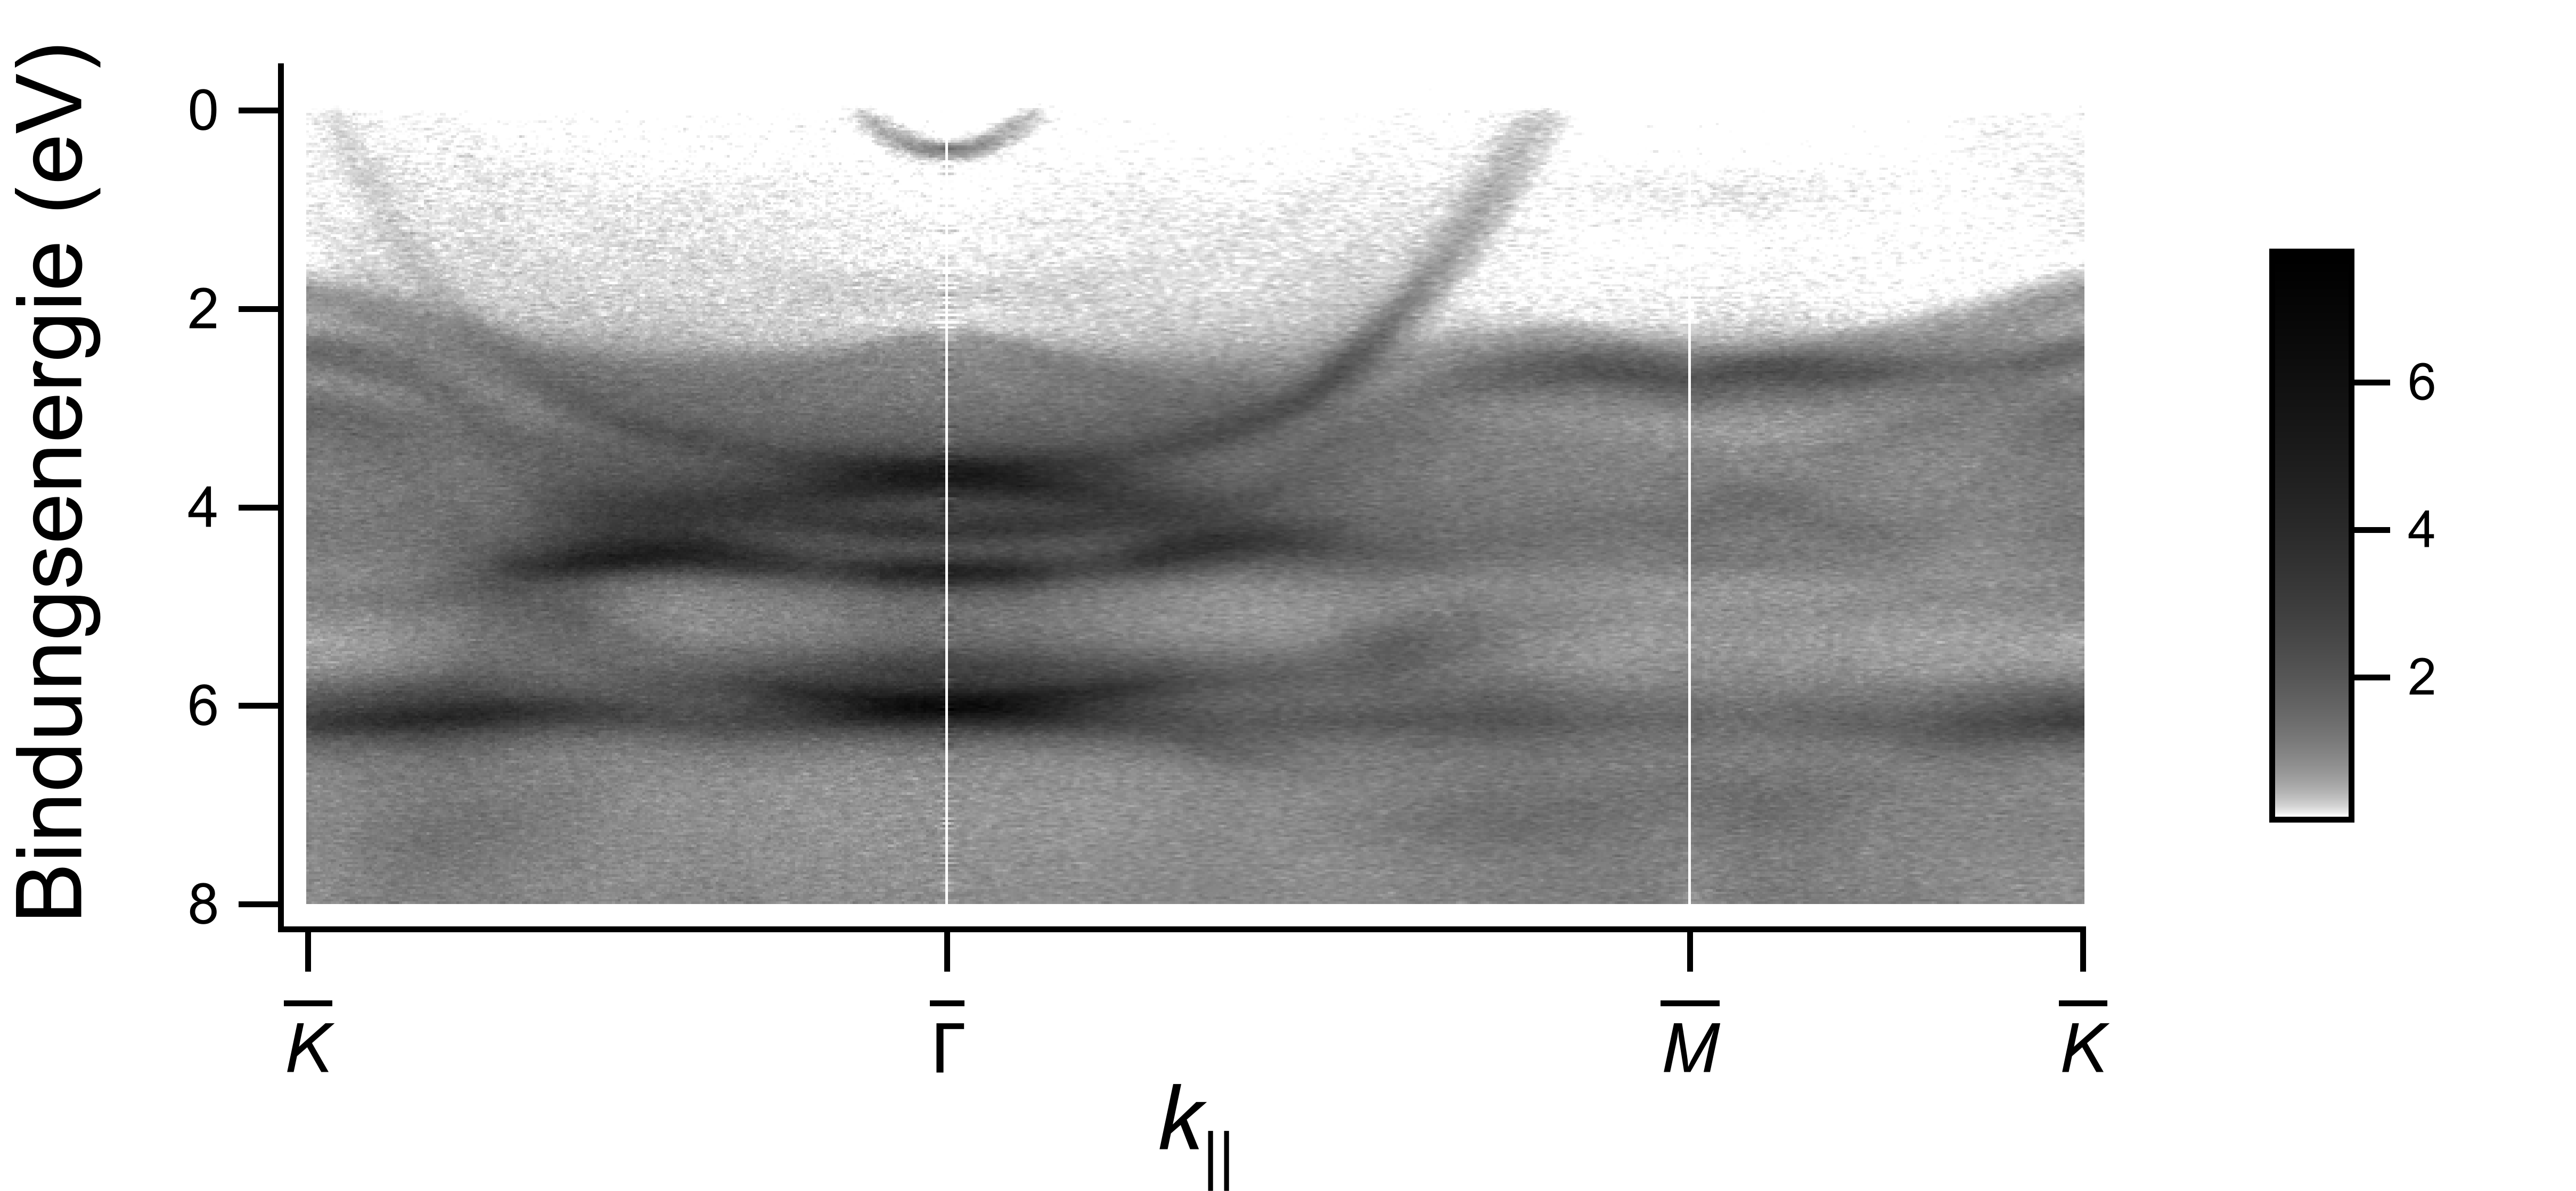
\includegraphics[height=3.74cm]{Au/Band_Au111.png}
                \subcaption{}
                \label{fig:Band_Au}
            \end{subfigure}
            \caption{Die gemessene Winkelverteilung von Gold (111) an der Fermifläche (\subref{fig:BZ_Au}).
            Eingezeichnet in rot ist die erste Brillouinzone und drei Hochsymmetriepunkte.
            In (\subref{fig:Band_Au}) ist die gemessene Bandstruktur von Gold (111) aufgetragen, welche sich durch Schneiden des dreidimensionale Datensatz entlang der orange gestrichelte Linien in (\subref{fig:BZ_Au}) ergibt.}
        \end{figure}
        Die Qualität der präparierten Goldoberfläche lässt sich ebenfalls mittels der PES bestimmen.
        Dafür wird der Oberflächenzustand verwendet, welcher zusätzlich mit der ersten Oberflächenbrillouinzone und den Hochsymmetriepunkten in \autoref{fig:BZ_Au} dargestellt ist.
        Nahe dem $\overline{\Gamma}$-Punkt befindet sich der Oberflächenzustand.
        Durch Schneiden entlang der orangen gestrichelten Linien zwischen den Hochsymmetriepunkten ergibt sich die Bandstruktur, welche in \autoref{fig:Band_Au} dargestellt ist.
        % So lassen sich dann auch die Merkmale in dem integrierten Spektrum aus \autoref{fig:EDC_Au+5A} für das Gold indetifizieren.
        Von der Fermikante bis hin zu etwa \SI{3.2}{\electronvolt} erstreckt sich parabelförmig das s-Band des Goldes.
        Im Bereich zwischen \SIrange{2}{6.2}{\electronvolt} befinden sich die fünf d-Bänder, welche durch ihre flache Form aufgrund der Lokalisierung der Elektronen erkennbar sind.

        \begin{figure}
            \centering
            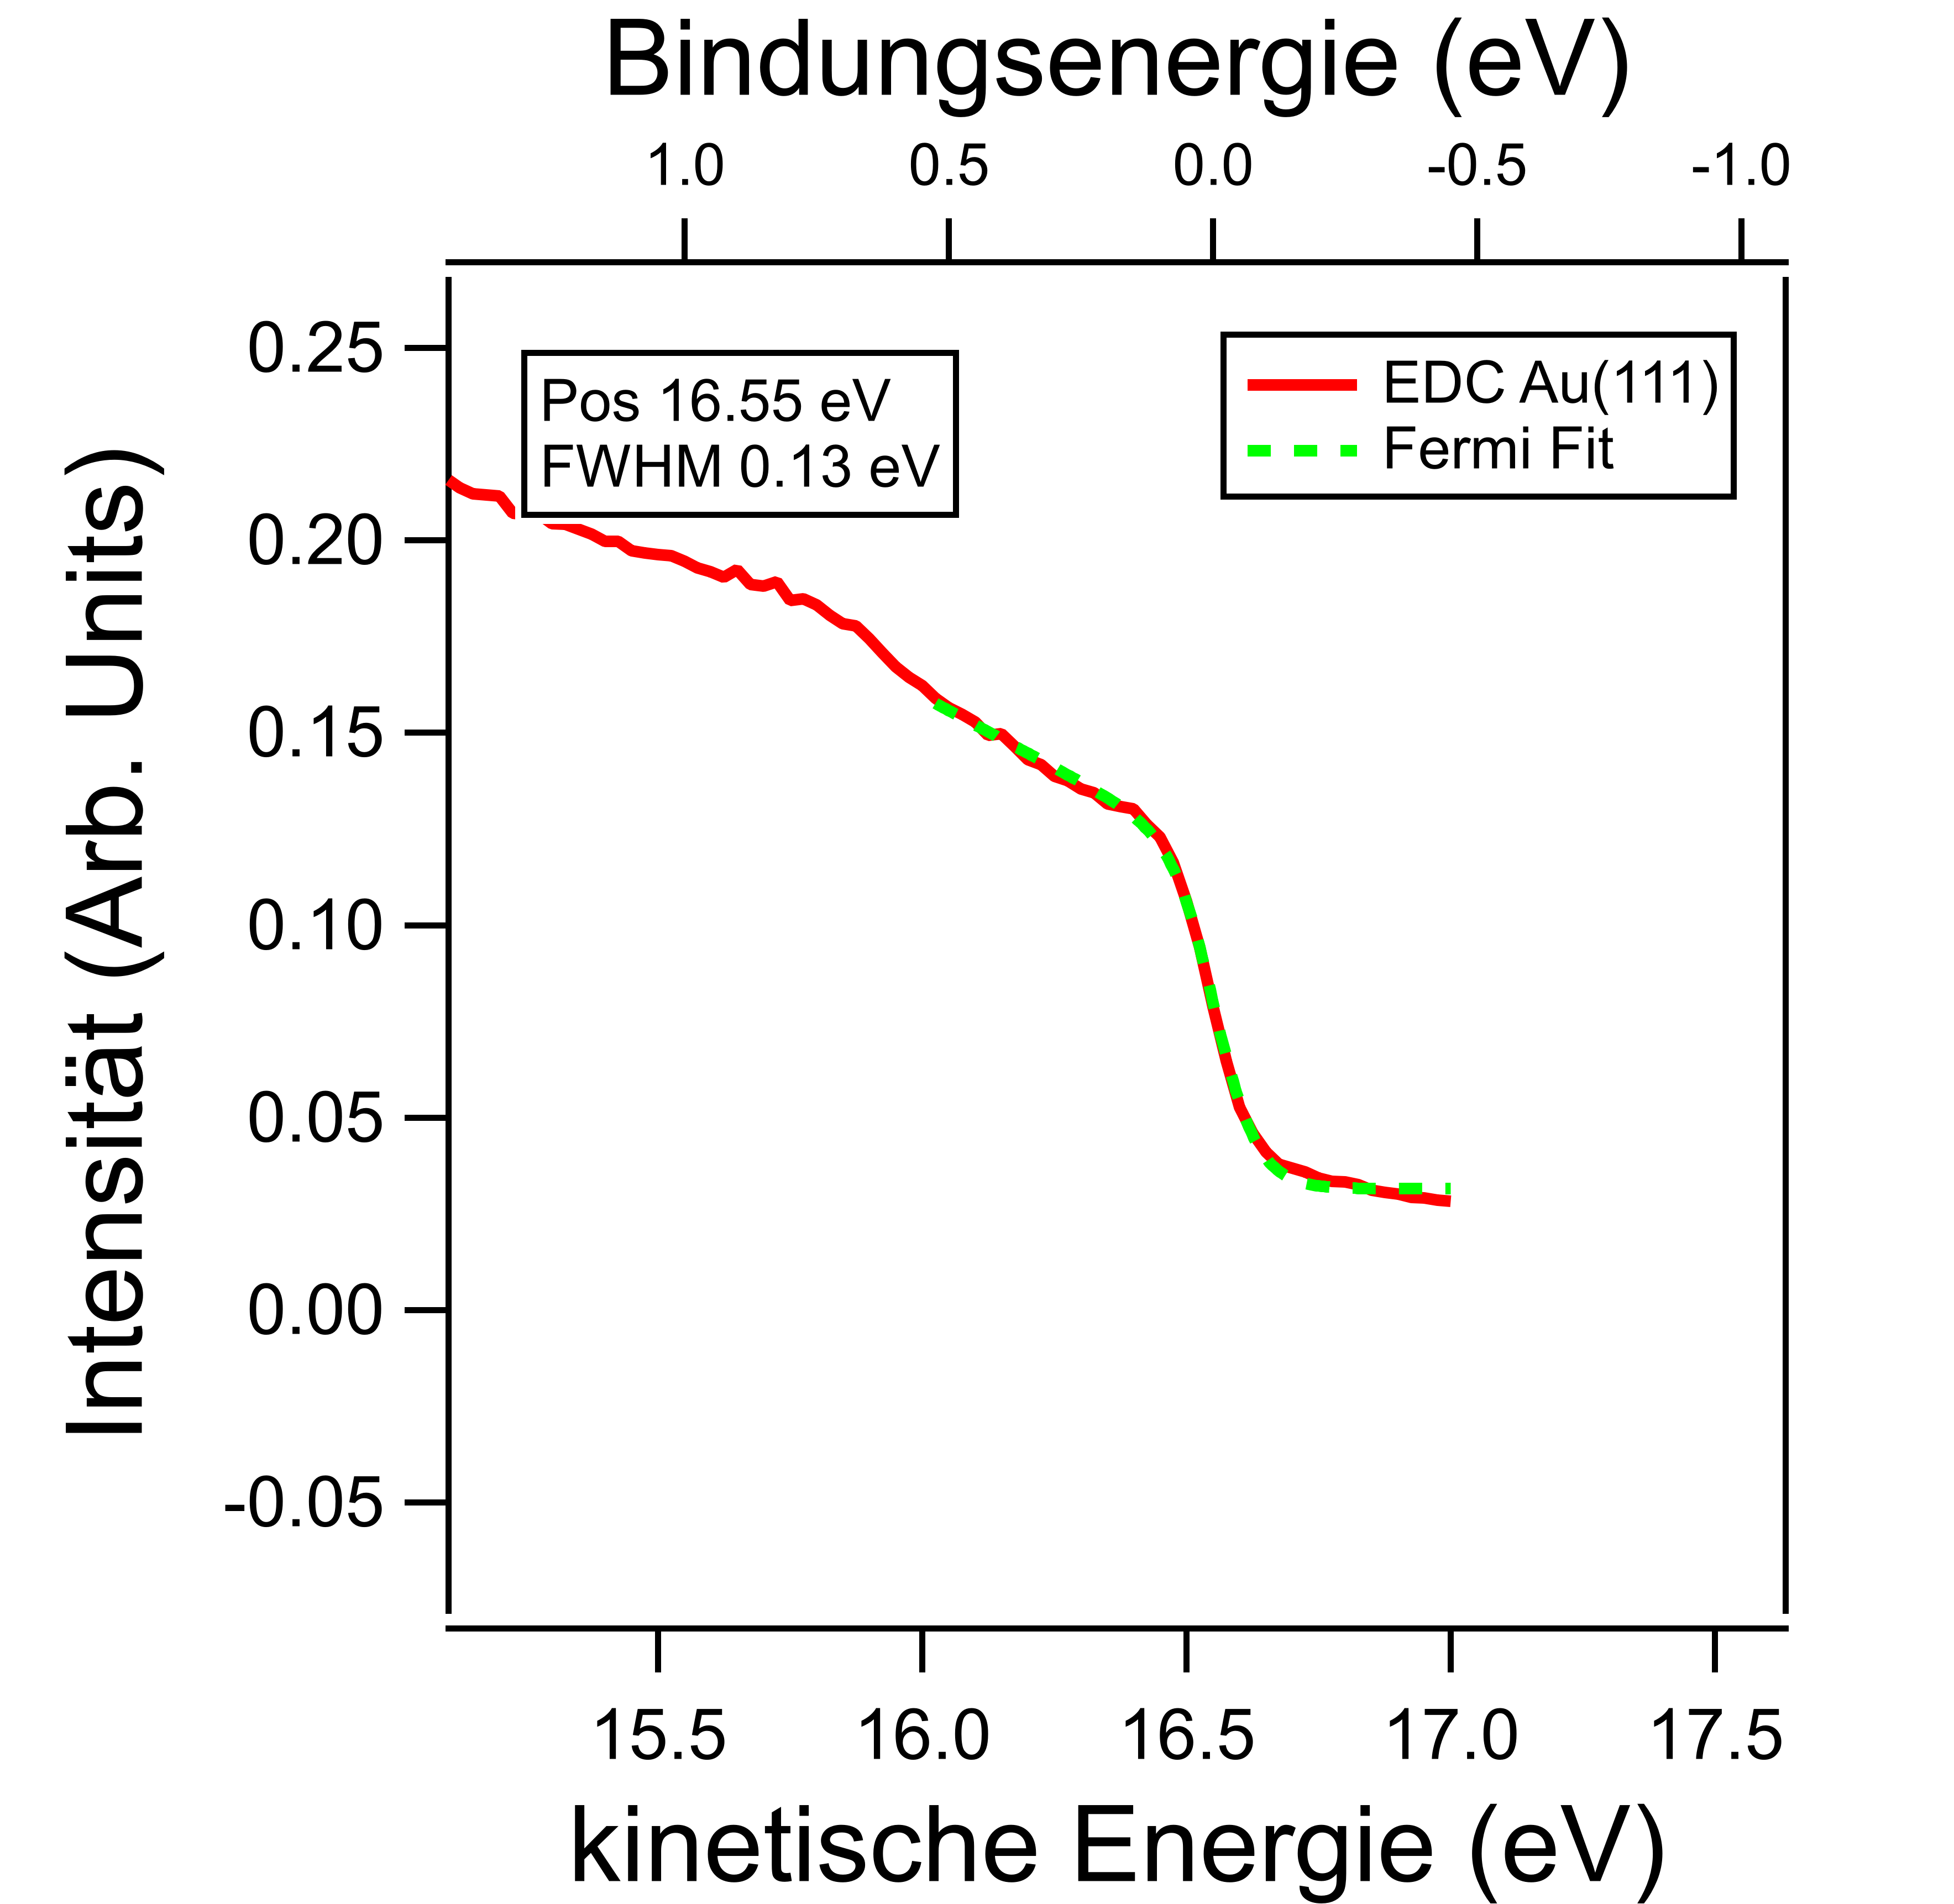
\includegraphics[width=0.5\textwidth]{Au/Fermi_Au.png}
            \caption{Das integrierte Spektrum an der Fermikante gemeinsam mit dem durchgeführtem Fit für das Gold.}
            \label{fig:Fermi_Au}
        \end{figure}
        Die Bindungsenergie wird mithilfe eines Fits der Fermikante in der EDC aus \autoref{fig:Fermi_Au} ermittelt.
        In dem die Photonenenergie von \SI{21.22}{\electronvolt} angenommen wird und die Fermikante des Goldes bei \SI{16.55}{\electronvolt} liegt, wird die Austrittsarbeit des Analysators zu \SI{4.72}{\electronvolt} bestimmt.
        Dies ist vor allem für die späteren Messungen des Nickeloxidfilms wichtig, da es sich hierbei um einen Isolator handelt und somit die Fermienergie in der Bandlücke liegt.
        Wird die gesamte Länge des Spektrums betrachtet, also der Energieunterschied zwischen Fermikante und Ende der Sekundärelektronen, so lässt sich die Austrittsarbeit der Probe bestimmen.
        Für die Austrittsarbeit des Goldes ergibt sich ein Wert von \SI{5.46}{\electronvolt}, was genau dem Literaturwerte entspricht~\cite{5A_4}.
        % Durch die Verschiebung des Abschnitt der Sekundärelektronen nach aufbringen des Pentacen ändert sich die Austrittsarbeit zu \SI{4.62}{\electronvolt}, was dabei sehr nah am Literaturwert von \SI{4.63}{\electronvolt} liegt~\cite{5A_4}.
        % Die Austrittsarbeit verschiebt sich also um \SI{0.84}{\electronvolt}, was auf ein starkes Oberflächendipolmoment hindeutet~\cite{5A_3}.
        % Auf Grund der Abwesenheit eines permaneten Dipols in den Molekülen und der Physisorption kann dies auf den Push-back Effekt zurück geführt werden.
   
        Der \ce{NiO}-Film wird durch das Aufdampfen von Nickel mit einer Rate von \SI{0.62}{\angstrom\per\minute} in einer Sauerstoffatmosphäre von \SI{2e-6}{\milli\bar} bei Raumtemperatur augebracht.
        \begin{figure}
            \centering
            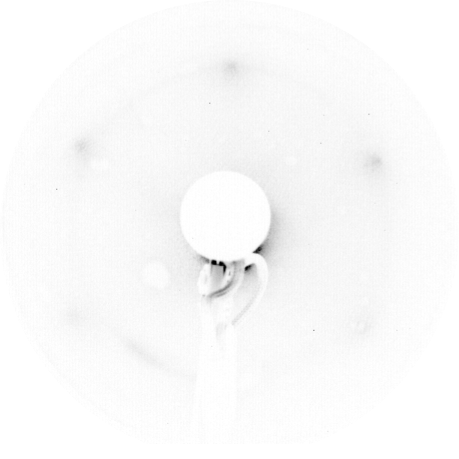
\includegraphics[height=5cm]{NiO/2021_06_15_019_NiO(111)_73eV_Thicklayer}
            \caption{Der Nickeloxidfilm (111) bei einer Elektronenenergie von \SI{73}{\electronvolt}.}
            \label{fig:LEED_NiO}
        \end{figure}
        Es ergibt sich das LEED-Bild in \autoref{fig:LEED_NiO}.
        Im Vergleich zu den klaren und scharfen Punkten des sauberen Gold scheinen diese ausgewaschen zu sein und die Reflexe der zweiten Ordnung sind verschwunden.
        Die Ursache daran liegt in der nicht ganz perfekten Oberflächenbeschaffenheit~\cite{NiO_34}.
        % Nun sind im oberen Bereich die Intensitäten der Reflexe beim Nickeloxid gleich groß, wohingegen im unteren Bereich nur noch schwache Intensitäten zu erkennen sind.
        Aufgrund ihrer nahezu gleichen Gitterkonstanten von Nickeloxid und Gold sind die radialen Positionen der Punkte unverändert.
        Durch die polare Oberflächennatur der (111)-Orientierung und der damit verbundenen Instabilität können verschiedene Relaxationsprozesse auftreten~\cite{NiO_36, NiO_35, NiO_34, NiO_27, NiO_10}.
        Aus der gleichen Symmetrie der Punkte und der Abwesenheit zusätzlicher Punkte kann eine $\text{p}(2 \times 2)$ Rekonstruktion~\cite{NiO_37}, sowie Domänenbildung der (100)-Orientierung~\cite{NiO_36} ausgeschlossen werden.
        Die hier wahrscheinlichste Stabilisierung der Oberfläche ist die \ce{OH-}-Terminierung mit der $\text{p}(1 \times 1)$-Rekonstruktion~\cite{NiO_35}.
        % Hierbei wird das Oberflächenpotential durch Reduzierung der Oberflächenladung verkleinert und die Oberfläche wird thermodynamisch stabil.

        \begin{figure}
            \centering
            \begin{subfigure}[t]{0.48\textwidth}
                \centering
                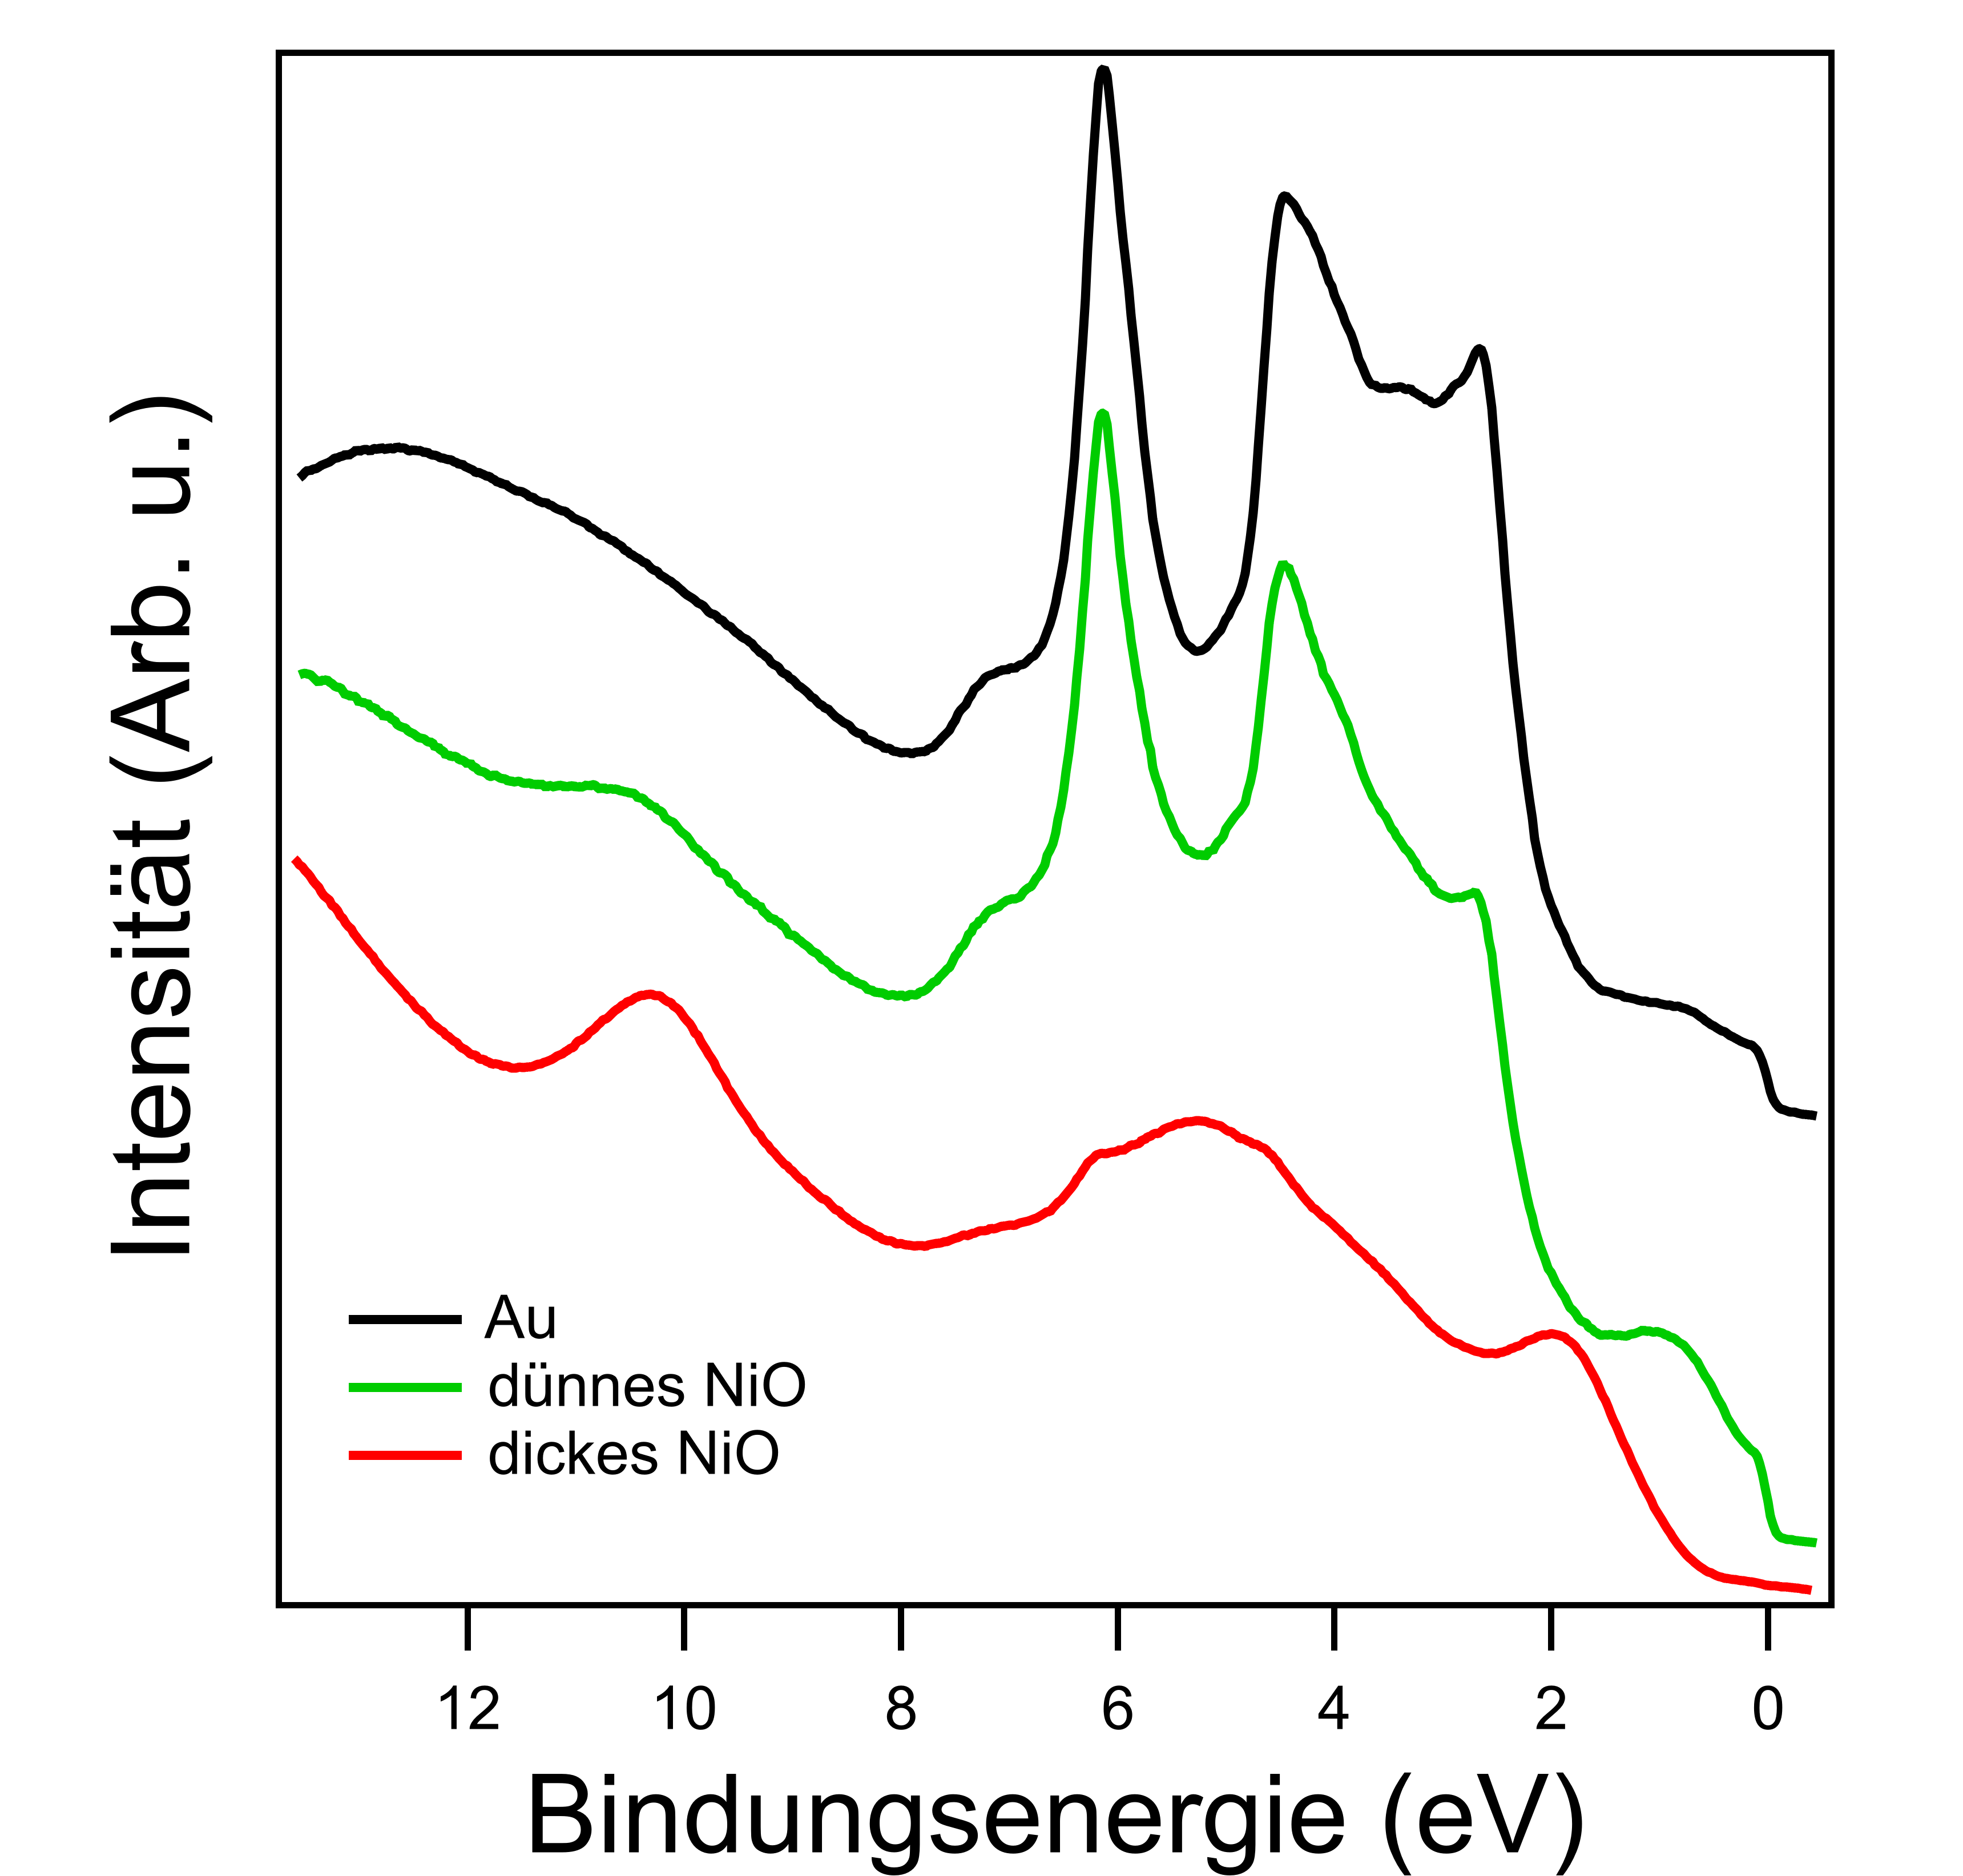
\includegraphics[height=5cm]{NiO/NiO_Filmdicke.png}
                \subcaption{}
                \label{fig:EDC_NiO}
            \end{subfigure}
            \begin{subfigure}[t]{0.48\textwidth}
                \centering
                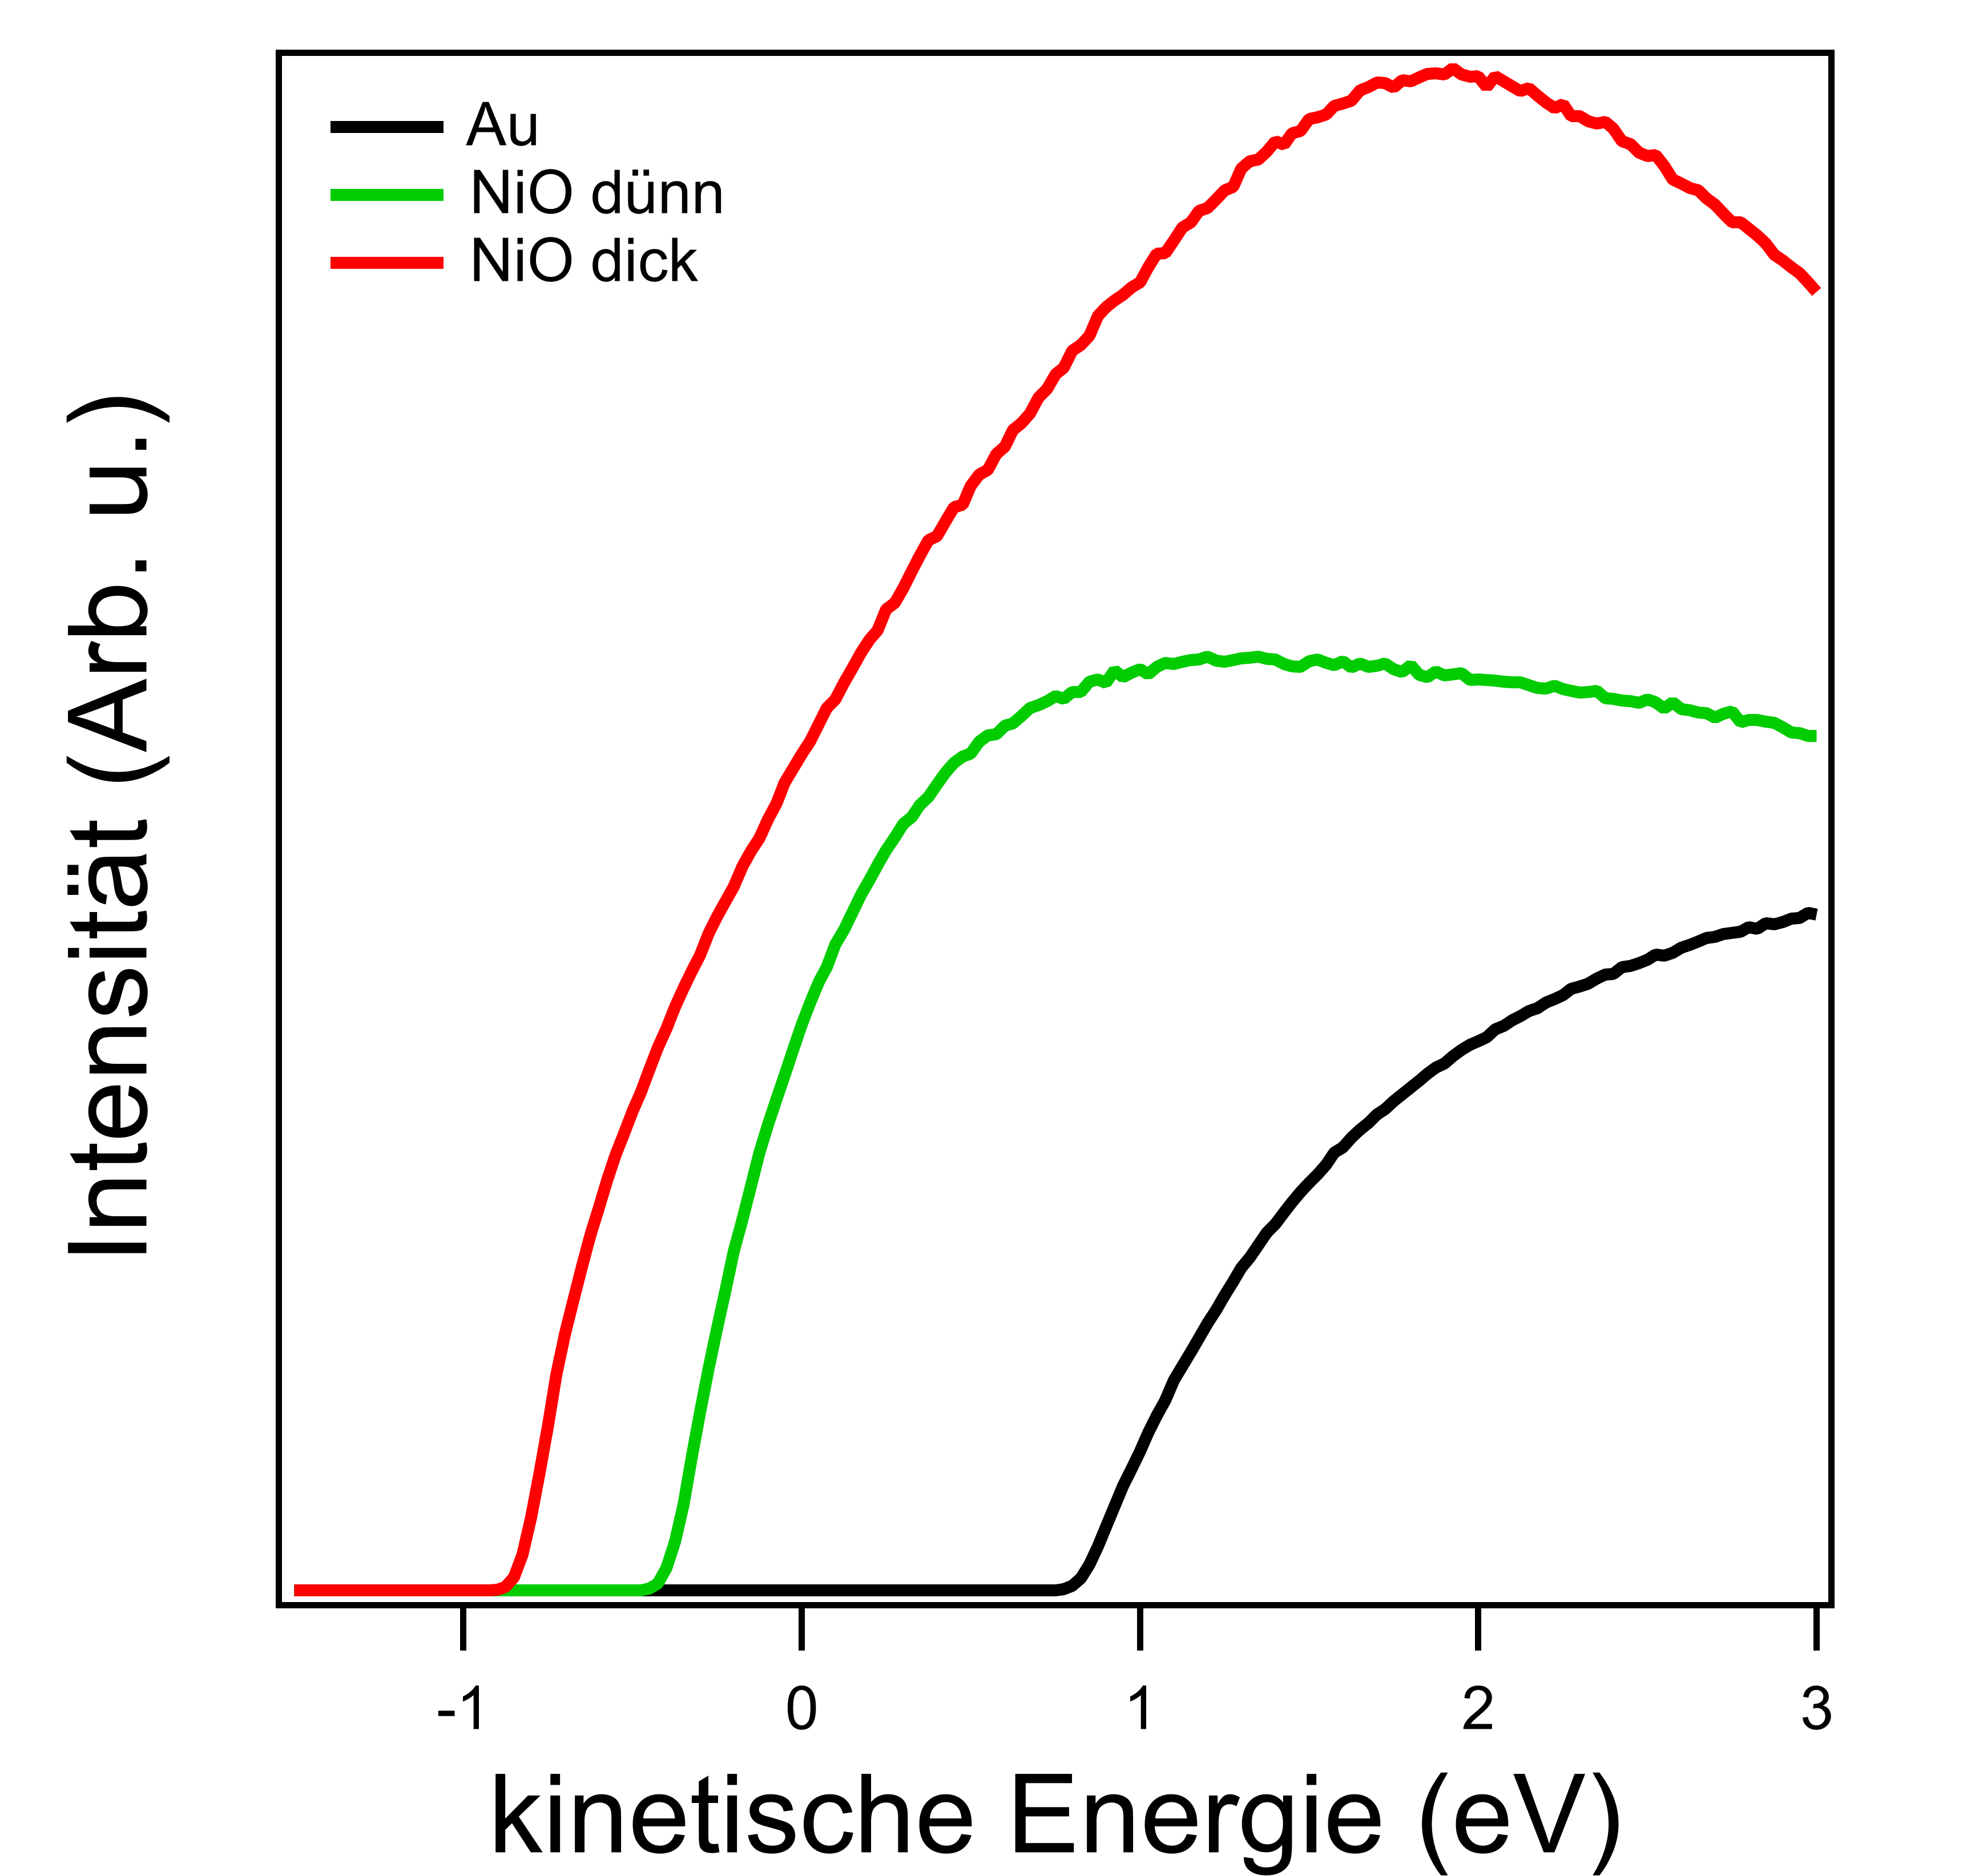
\includegraphics[height=5cm]{NiO/WKF_thickness.png}
                \caption{}
                \label{fig:WKF_NiO}
            \end{subfigure}
            \caption{(\subref{fig:EDC_NiO}) Die integrierten Spektren für zwei verschiedene Schichtdicken von \ce{NiO}. Als Referenz dient das integrierte Spektrum von Gold. 
            (\subref{fig:WKF_NiO}) Die integrierten Spektren im Bereich der Sekundärelektronen für verschiedene Schichtdicken von \ce{NiO}.}
        \end{figure}
        Durch die Variation der Aufdampfzeiten lassen sich zwei verschiedene Schichtdicken von ca. \SI{16}{\angstrom} und \SI{37}{\angstrom} erzeugen.
        Für diese beiden Dicken sind die winkelintegrierten Spektren des Valenzbandbereiches in \autoref{fig:EDC_NiO} gemeinsam mit dem Spektrum des Substrates dargestellt.
        Zu erkennen ist, dass mit zunehmender Schichtdicke die charakteristischen Merkmale des Substrates, genauer der d-Bändern abnehmen, aber nicht vollständig verschwinden.
        Dafür steigt das Signal, welches vom Nickeloxid herrührt an (Vergleich \autoref{fig:EDC_NiO_thick}).
        Aus der Verschiebung des Punktes an dem die Sekundärelektronen aufhören lässt sich erkennen, dass sich die Austrittsarbeit vom Gold mit steigender Schichtdicke des Nickeloxid zu kleineren Werten hin verschiebt.
        Dies ist in \autoref{fig:WKF_NiO} für verschiedene Aufdampfzeiten dargestellt.
        Eine negative kinetische Energie kann dadurch erklärt werden, dass die Probe auf einem zusätzlichen Potential liegt.
        Vom dünnen Nickeloxidfilm zum dickeren Nickeloxidfilm wechselt die Austrittsarbeit von \SI{4.25}{\electronvolt} zu \SI{3.80}{\electronvolt}.
        % Kleine Verschiebungen könnten durch unterschiedliche Aufdampfbedingungen erklärt werden, hier rührt 
        Die Verschiebung kann durch die Ausbildung des Oberflächendipolmomentes kommen~\cite{5A_5}.
        Eine weitere Verringerung der Austrittsarbeit wird durch Adsorbate, wie die \ce{OH-}-Terminierung hervorgerufen~\cite{NiO_40}.
        % Weitere Verunreinigungen können durch die verwendete Heliumlampe auftreten, da der Druck in der Analysekammer stark ansteigt.
        Dabei liegt die ermittelte Austrittsarbeit des dicken Nickeloxidfilms unterhalb des erwarteten Bereichs von \SIrange{4.5}{5.2}{\electronvolt}~\cite{poulain_electronic_2020}.
        Eine Verringerung der Austrittsarbeit kann dabei auf Sauerstofffehlstellen, welche als negative Defekte gelten erklärt werden~\cite{IF_3}.
        % Die Erniedrigung der Austrittsarbeit geht auch ein her mit der Ausbildung eines Oberflächendipolmomentes, was für Nickeloxid in der (111)-Orientierung erwartet wird~\cite{5A_5}.
        Durch Manipulation des Aufdampfprozesses können so gezielt bestimmte elektronische Eigenschaft, wie zum Beispiel die Austrittsarbeit verändert werden~\cite{poulain_electronic_2020}.

        \begin{figure}
            \centering
            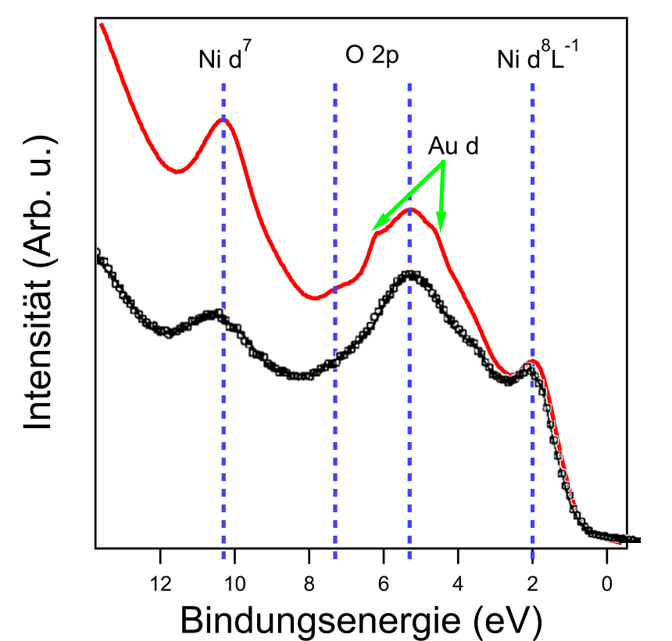
\includegraphics[height=7cm]{NiO/EDC_NiO_thick+exp.png}
            \caption{Winkelintegriertes Spektrum des dicken Nickeloxidfilms (rot), gemeinsam mit den identifizierten Merkmalen (blau).
            Überlagert dargestellt (schwarz) ist das gemessene Spektrum von Marre und Neddermeyer~\cite{NiO_7}.} 
            \label{fig:EDC_NiO_thick}
        \end{figure}
        In der \autoref{fig:EDC_NiO_thick} ist das Valenzbandspektrum des dicken Nickeloxidfilms aufgetragen.
        Ebenfalls sind die Zuordnungen des Ursprungs der Merkmale gekennzeichnet, wobei L für den Ligandenzustand steht.
        % Bei einem Vergleich zwischen der gemessenen Kurve und der von Marre und Neddermeyer~\cite{NiO_7} fällt auf, dass es eine konstante Verschiebung gibt.
        % Ursache könnte die Bestimmung der Fermikante sein. %  denn bei Nickeloxid handelt es sich um einen Isolator und folglich liegt das Ferminiveau in der Bandlücke.
        Die strukturelle Übereinstimmung ist klar zu erkennen. 
        Ferner fällt auf, dass die Elemente des Übergangsmetalls deutlich präsenter sind als in der Referenz.
        % Dies wiederrum ist in guter Übereinstimmung mit der Annahme von Sauerstofffehlstellen.
        Bei höheren Bindungsenergien bleibt die strukturelle Übereinstimmung erhalten, obwohl sich deutliche Intensitätsunterschiede zeigen.
        Diese Abweichung kann durch den unterschiedlichen Untergrund, der durch die Sekundärelektronen hervorgerufen wird erklärt werden.
        % Die einzelnen Merkmale lassen sich dabei ihrer Herkunft zuordnen. 
        Bei \SI{2}{\electronvolt} wird die Intensität durch den hybridisierten Zustand aus dem Nickel $\text{d}^8$ Zustand mit dem Sauerstoff p Zustand dominiert.
        Das Sauerstoff 2p-Orbital hingegen dominiert den Bereich bei \SIrange[range-phrase=\:und\:]{5.3}{7.3}{\electronvolt}.
        Der Nickel $\text{d}^7$ Zustand zeigt dabei ein klares Signal bei \SI{10.3}{\electronvolt}.

        \begin{figure}
            \centering
            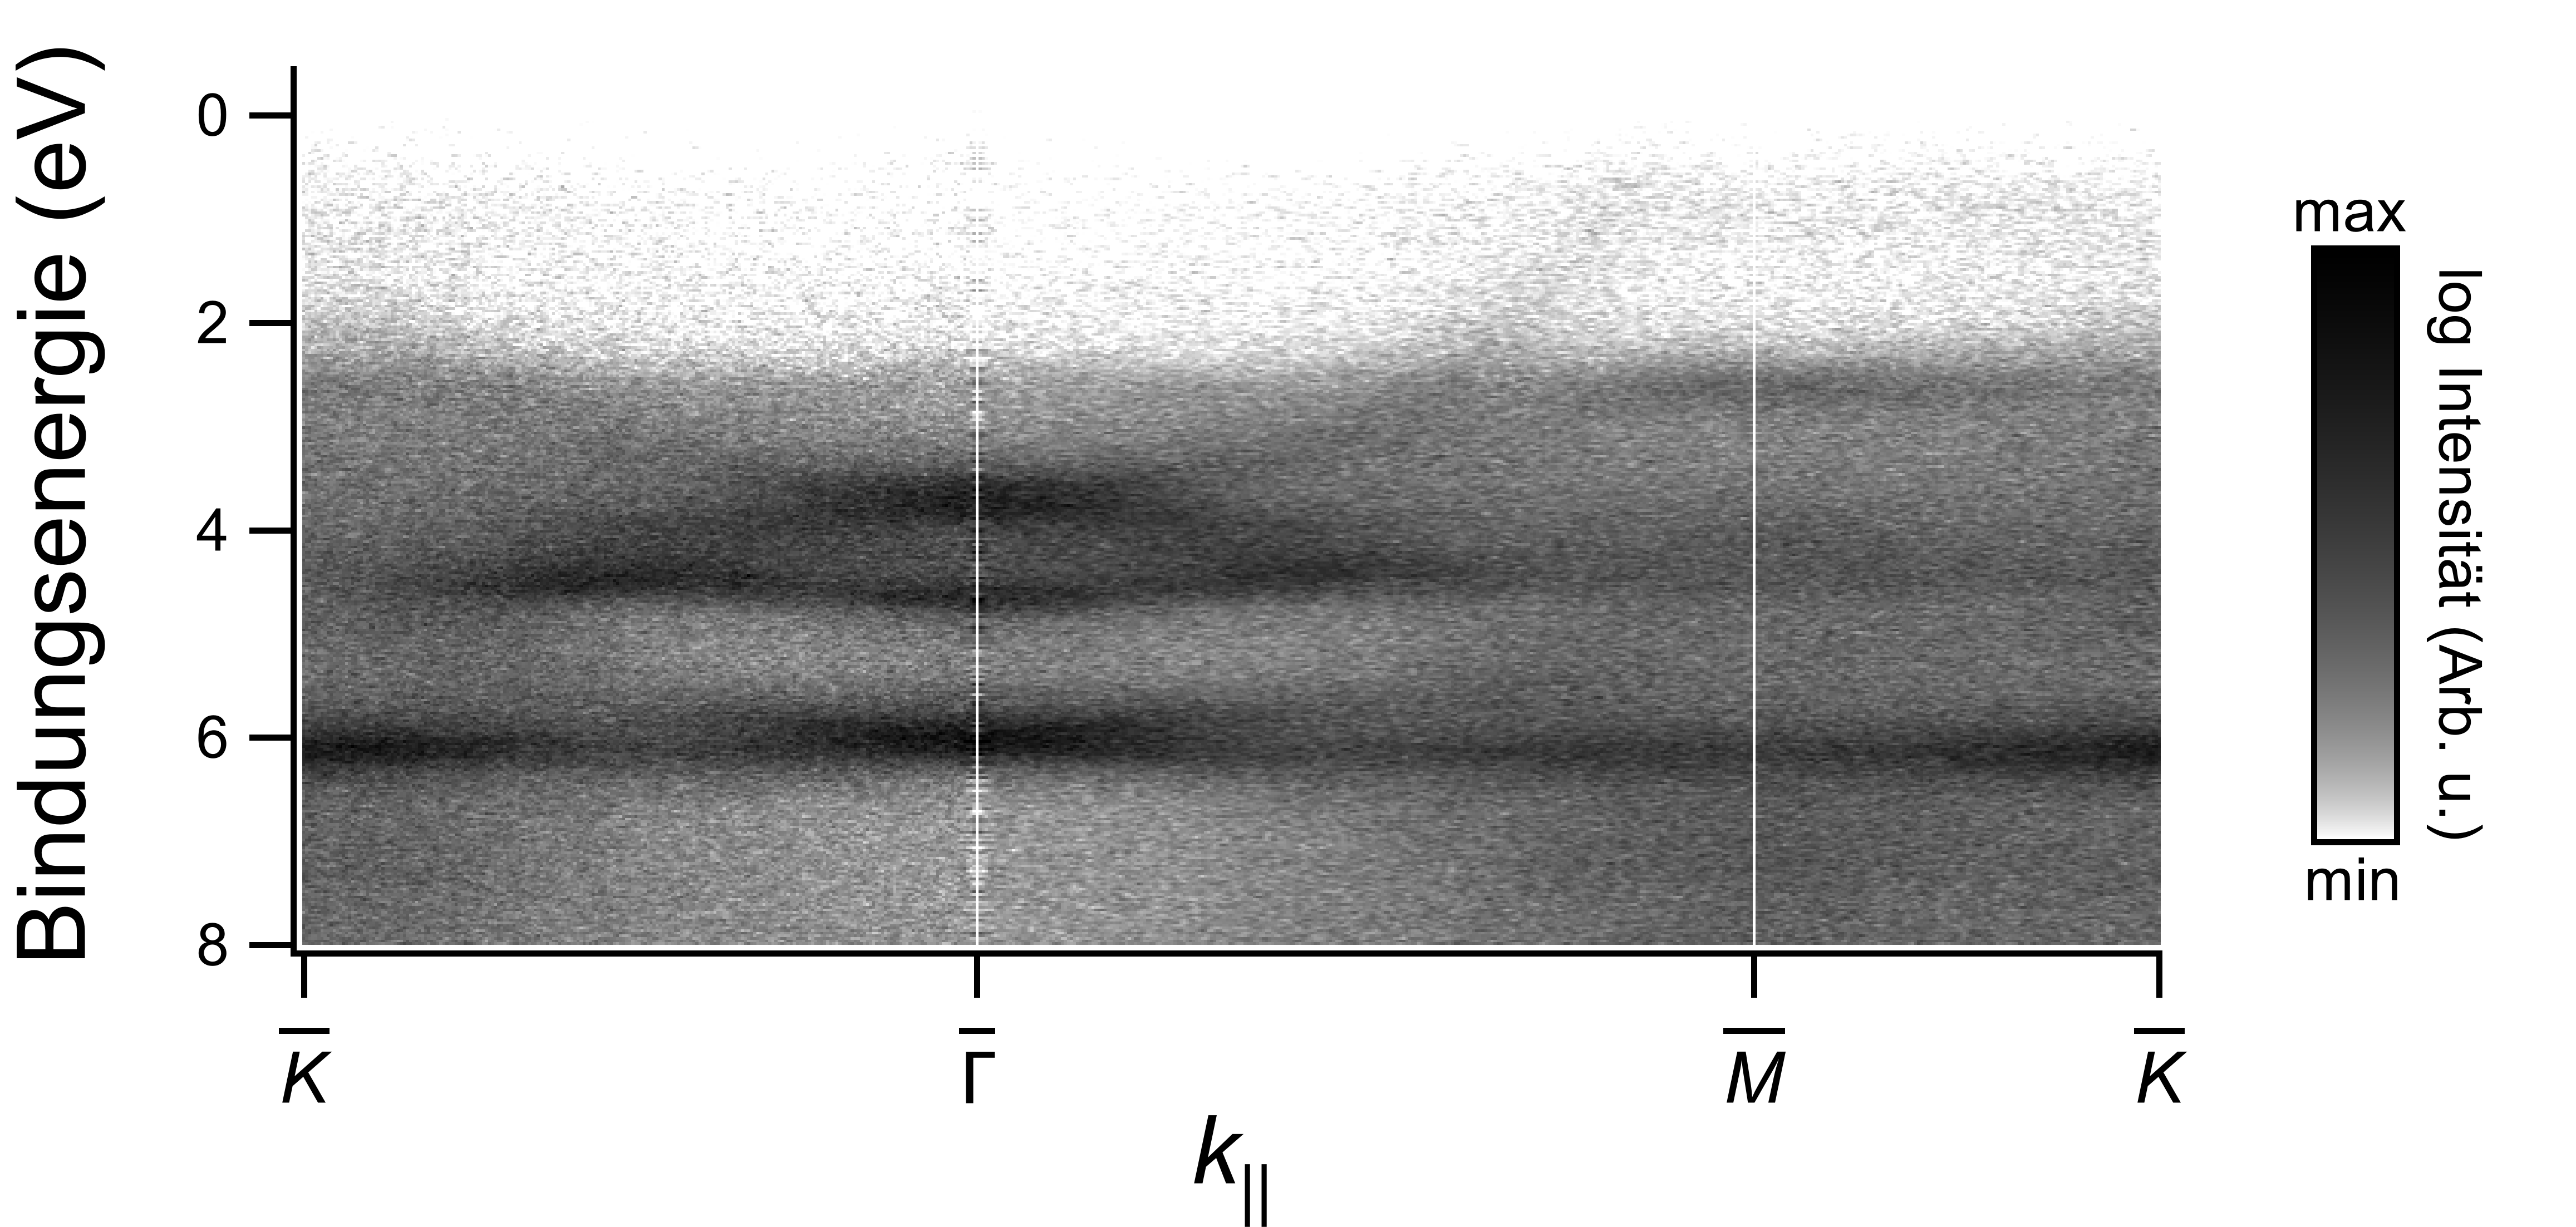
\includegraphics[height=4cm]{NiO/Band_NiO.png}
            \caption{Die gemessene Bandstruktur des dicken Nickeloxidfilms.}
            \label{fig:Band_NiO}
        \end{figure}
        Auch für Nickeloxid lässt sich aus dem dreidimensionalen Datensat die Bandstruktur extrahieren.
        Diese ist in \autoref{fig:Band_NiO} dargestellt. %, auf die Darstellung der Oberflächenbrillouinzone wird verzichtet, da sich lediglich die Länge der Linien im Vergleich zum Gold verändert.
        Der Oberflächenzustand des Goldes ist verschwunden, da nun sich Nickeloxid auf der Oberfläche befindet.
        Im Bereich zwischen Fermikante und etwa \SI{3.5}{\electronvolt} ist noch das s-Band des Goldes zu erkennen, da hier keine Struktur vom Nickeloxid erwartet wird~\cite{NiO_12}.
        In den Bereichen \SI{2}{\electronvolt}, \SI{4}{\electronvolt} und \SI{6}{\electronvolt} lassen sich jeweils ein bis zwei flach verlaufende Bänder erkennen.
        Das nahezu gerade Band bei \SI{2}{\electronvolt} lässt sich dabei klar dem hybridisierten Nickel d-Band zuordnen, da es nur schwach dispersiv ist, wohingegen die starken Intensitäten bei \SI{6}{\electronvolt} sich dem Sauerstoff 2p zuordnen lassen, wie es schon beim integrierten Spektrum in \autoref{fig:EDC_NiO_thick} geschehen ist.
        Eine eindeutige Zuordnung ob die Beiträge vom Gold und Nickeloxid kommen ist schwierig, da die Signale sich überlagern. % Nahe der Fermikante Effekte auftreten, die nicht vom \ce{NiO} herrühren können.
        Dies lässt sich ebenfalls an der EDC erkennen, dort sind vor allem für die d-Bänder des Goldes noch Beiträge sichtbar.
        
    \FloatBarrier
    \section{Eisenmonooxid} \label{sec:Prep_FeO}
        Um den Film aus Eisenmonooxid herzustellen wird als Substrat ein dünner Eisenfilm auf einer \ce{MgO}(100)-Oberfläche verwendet.
        Zunächst wird die Eisenprobe mittels leichten ioneninduzierten Zerstäubens und Aufheizen auf \SI{600}{\celsius} gereinigt
        % Auf diesen wird ein Film Magnetit aufgedampft und mittels Heizens und ioneninduziertem Zerstäuben in Eisenmonooxid umgewandelt.
        \begin{figure}
            \centering
            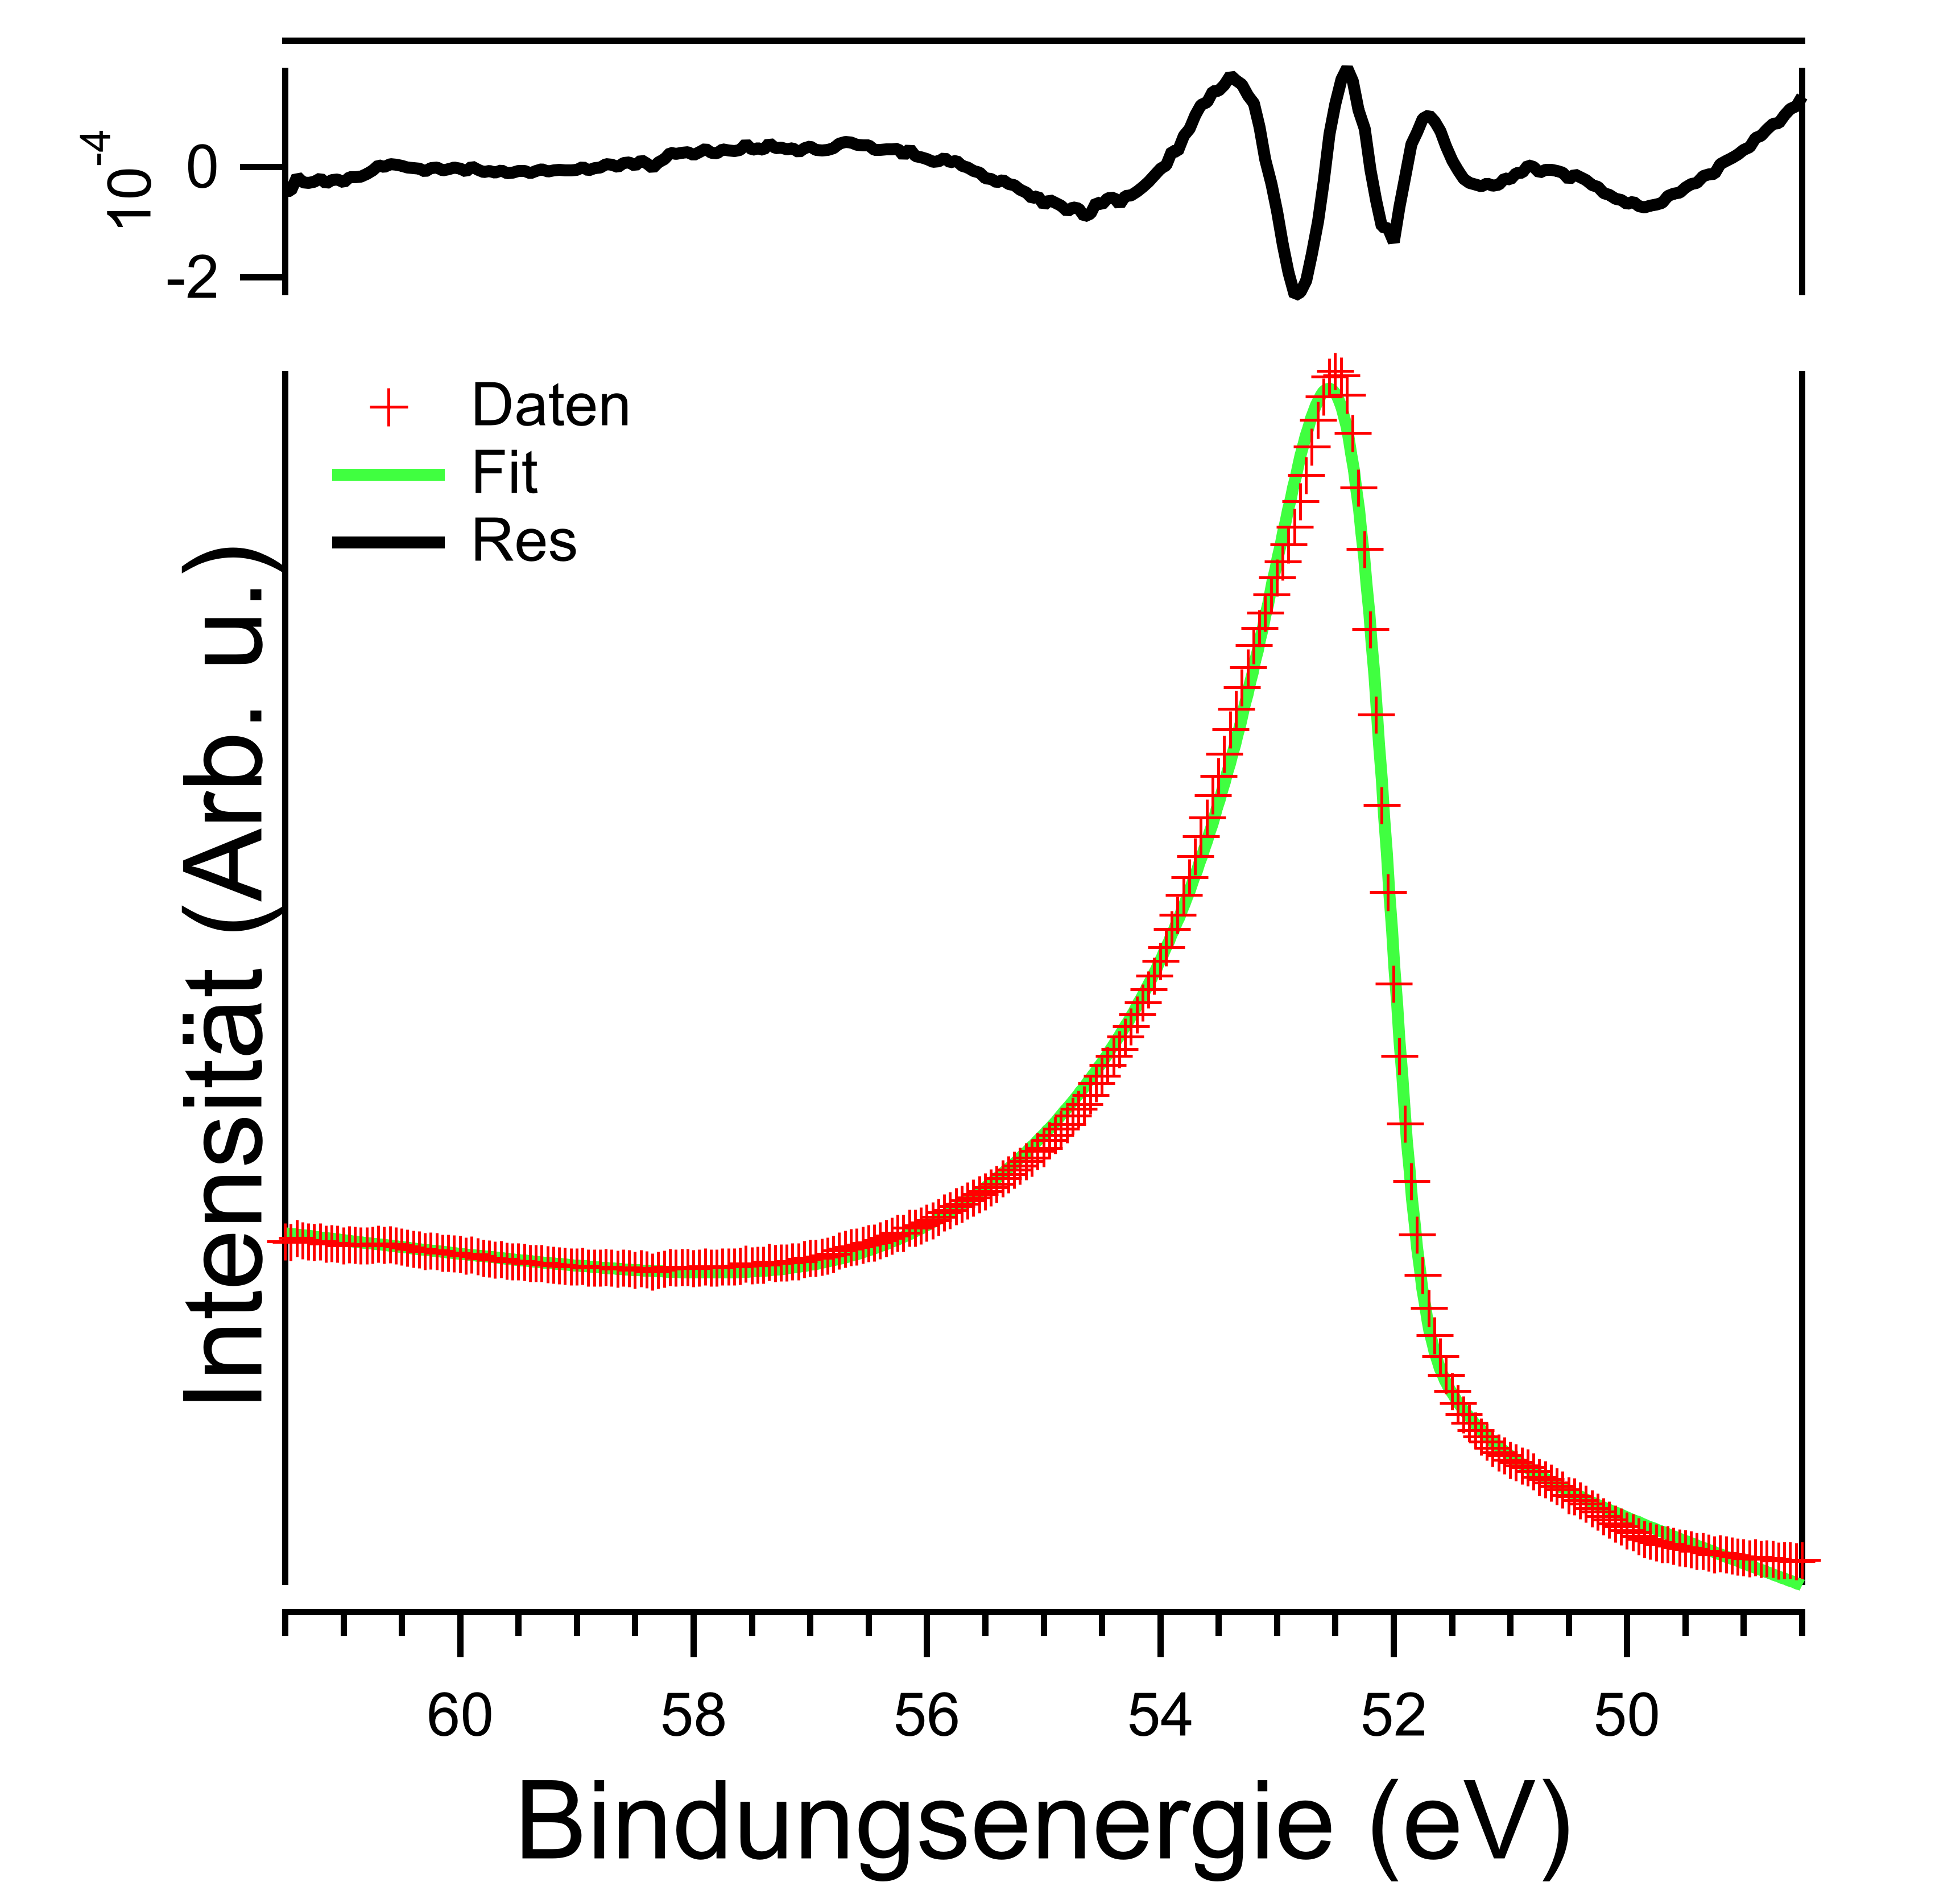
\includegraphics[width=0.5\textwidth]{Fe/Fe3p_Fe_2.png}
            \caption{XPS Spektrum des $\ce{Fe}_{3\text{p}}$-Zustand des reinen Eisens bei Raumtemperatur und einer Photonenenergie von \SI{200}{\electronvolt}.}
            \label{fig:XPSFe3p_Fe}
        \end{figure}
        Die Reinheit der Probe lässt sich am XPS-Spektrum des $\ce{Fe}_{3\text{p}}$-Signals in \autoref{fig:XPSFe3p_Fe} erkennen.
        Das Signal bei \SI{52.83}{\electronvolt} lässt sich nach Abzug eines Pseudo-Tougaard Untergrunds sehr gut mit einer Pseudo-Voigt Funktion approximieren~\cite{schmid_new_2014}.
        Die ermittelte Position des $\ce{Fe}_{3\text{p}}$-Signals passt zur Literatur mit einer Position von \SI{53.8}{\electronvolt} und einer Halbwertsbreite von \SI{1.73}{\electronvolt}~\cite{FeO_50}.
        Hierbei ist die gemessene Halbwertsbreite mit \SI{2.11}{\electronvolt} etwas größer, dennoch im Akzeptanzbereich, da eine Spin-Bahn-Aufspaltung bei der Wahlt der beitragenden Voigt-Funktionen vernachlässigt wurde. % , wobei die Probe auch bei Raumtemperatur vermessen wurde.
        In diesem wie auch den folgenden Spektren von Kernniveaus zeigt das Residium bei steigender Flanke einige Oszillationen auf, dessen Ursache nicht bekannt ist.
        Da es stets (hier und in den folgenden XPS-Spektren) bei steigender Flanke und einer gleichen Form von etwa \num{3} Wellenzügen auftritt, ist davon auszugehen, dass es sich nicht nur um Rauschen handelt, sondern eine systematische Ursache hat.

        Um ebenfalls die kinetische Energie in die übliche Bindungsenergie umzurechnen, muss die Austrittsarbeit des Analysators bestimmt werden.
        Dies ist nötig, da es sich bei den Eisenmonooxid, wie auch dem Magnetit bei der Messtemperatur von \SI{90}{\kelvin}, um einen Isolator handelt und hier die Fermikante nicht ermittelt werden kann.
        Aus der Anpassung an der Fermikante des Eisens lässt sich die Position der Fermikante auf \SI{59.5}{\electronvolt} bei einer Photonenenergie von \SI{64}{\electronvolt} bestimmen.
        Dadurch lässt sich für die spätere Umrechnung in die Bindungsenergie die Austrittsarbeit des Analysators bei NanoESCA auf \SI{4.5}{\electronvolt} festlegen. 
        % \textbf{nach Vitaly liegt die bei 4,25eV (kann sich aber nach dem Flashen ändern~\cite{vickerman_surface_2009})}
        Anzumerken ist, dass die Genauigkeit dieser Annahme nicht exakt ist, da zusätzlich die Fermikante durch ein starkes Signal von den d-Bändern überlagert wird.
        % Aus dem Abschnitt der Sekundärelektronen lässt sich die Austrittsarbeit der passivierten Eisenprobe auf \SI{4.06}{\electronvolt} bestimmen.

        \begin{figure}
            \begin{subfigure}[t]{0.34\textwidth}
                \centering
                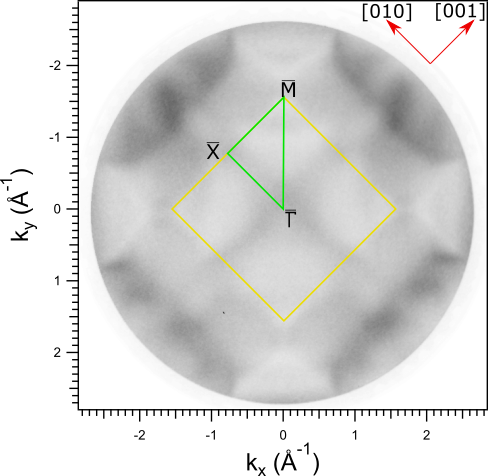
\includegraphics[height=4cm]{Fe/BZ_Fe.png}
                \subcaption{}
                % Die Brillouinzone des reinen Eisens bei einer Bindungsenergie von \SI{0.3}{\electronvolt}.
                % Eigezeichnet sind auch die Vektoren, sowie einige Hochsymmetrierichtungen.
                % Die Kantenlänge der BZ ist $\frac{2\pi}{a} = \SI[per-mode=reciprocal]{2.20}{\per\angstrom}$.
                % Im Zentrum liegt der $\overline{\Gamma}$-Punkt, der Abstand zum $\overline{X}$-Punkt ist $\frac{2\pi}{2 \cdot a} = \SI[per-mode=reciprocal]{1.10}{\per\angstrom}$ und zum $\overline{M}$-Punkt $\frac{2\pi}{2 \cdot a} \sqrt{2} = \SI[per-mode=reciprocal]{1.55}{\per\angstrom}$.
                % Verwendete Photonenenergie war \SI{64}{\electronvolt} und die Polarisation p.
                \label{fig:BZ_Fe}
            \end{subfigure}
            \begin{subfigure}[t]{0.62\textwidth}
                \centering
                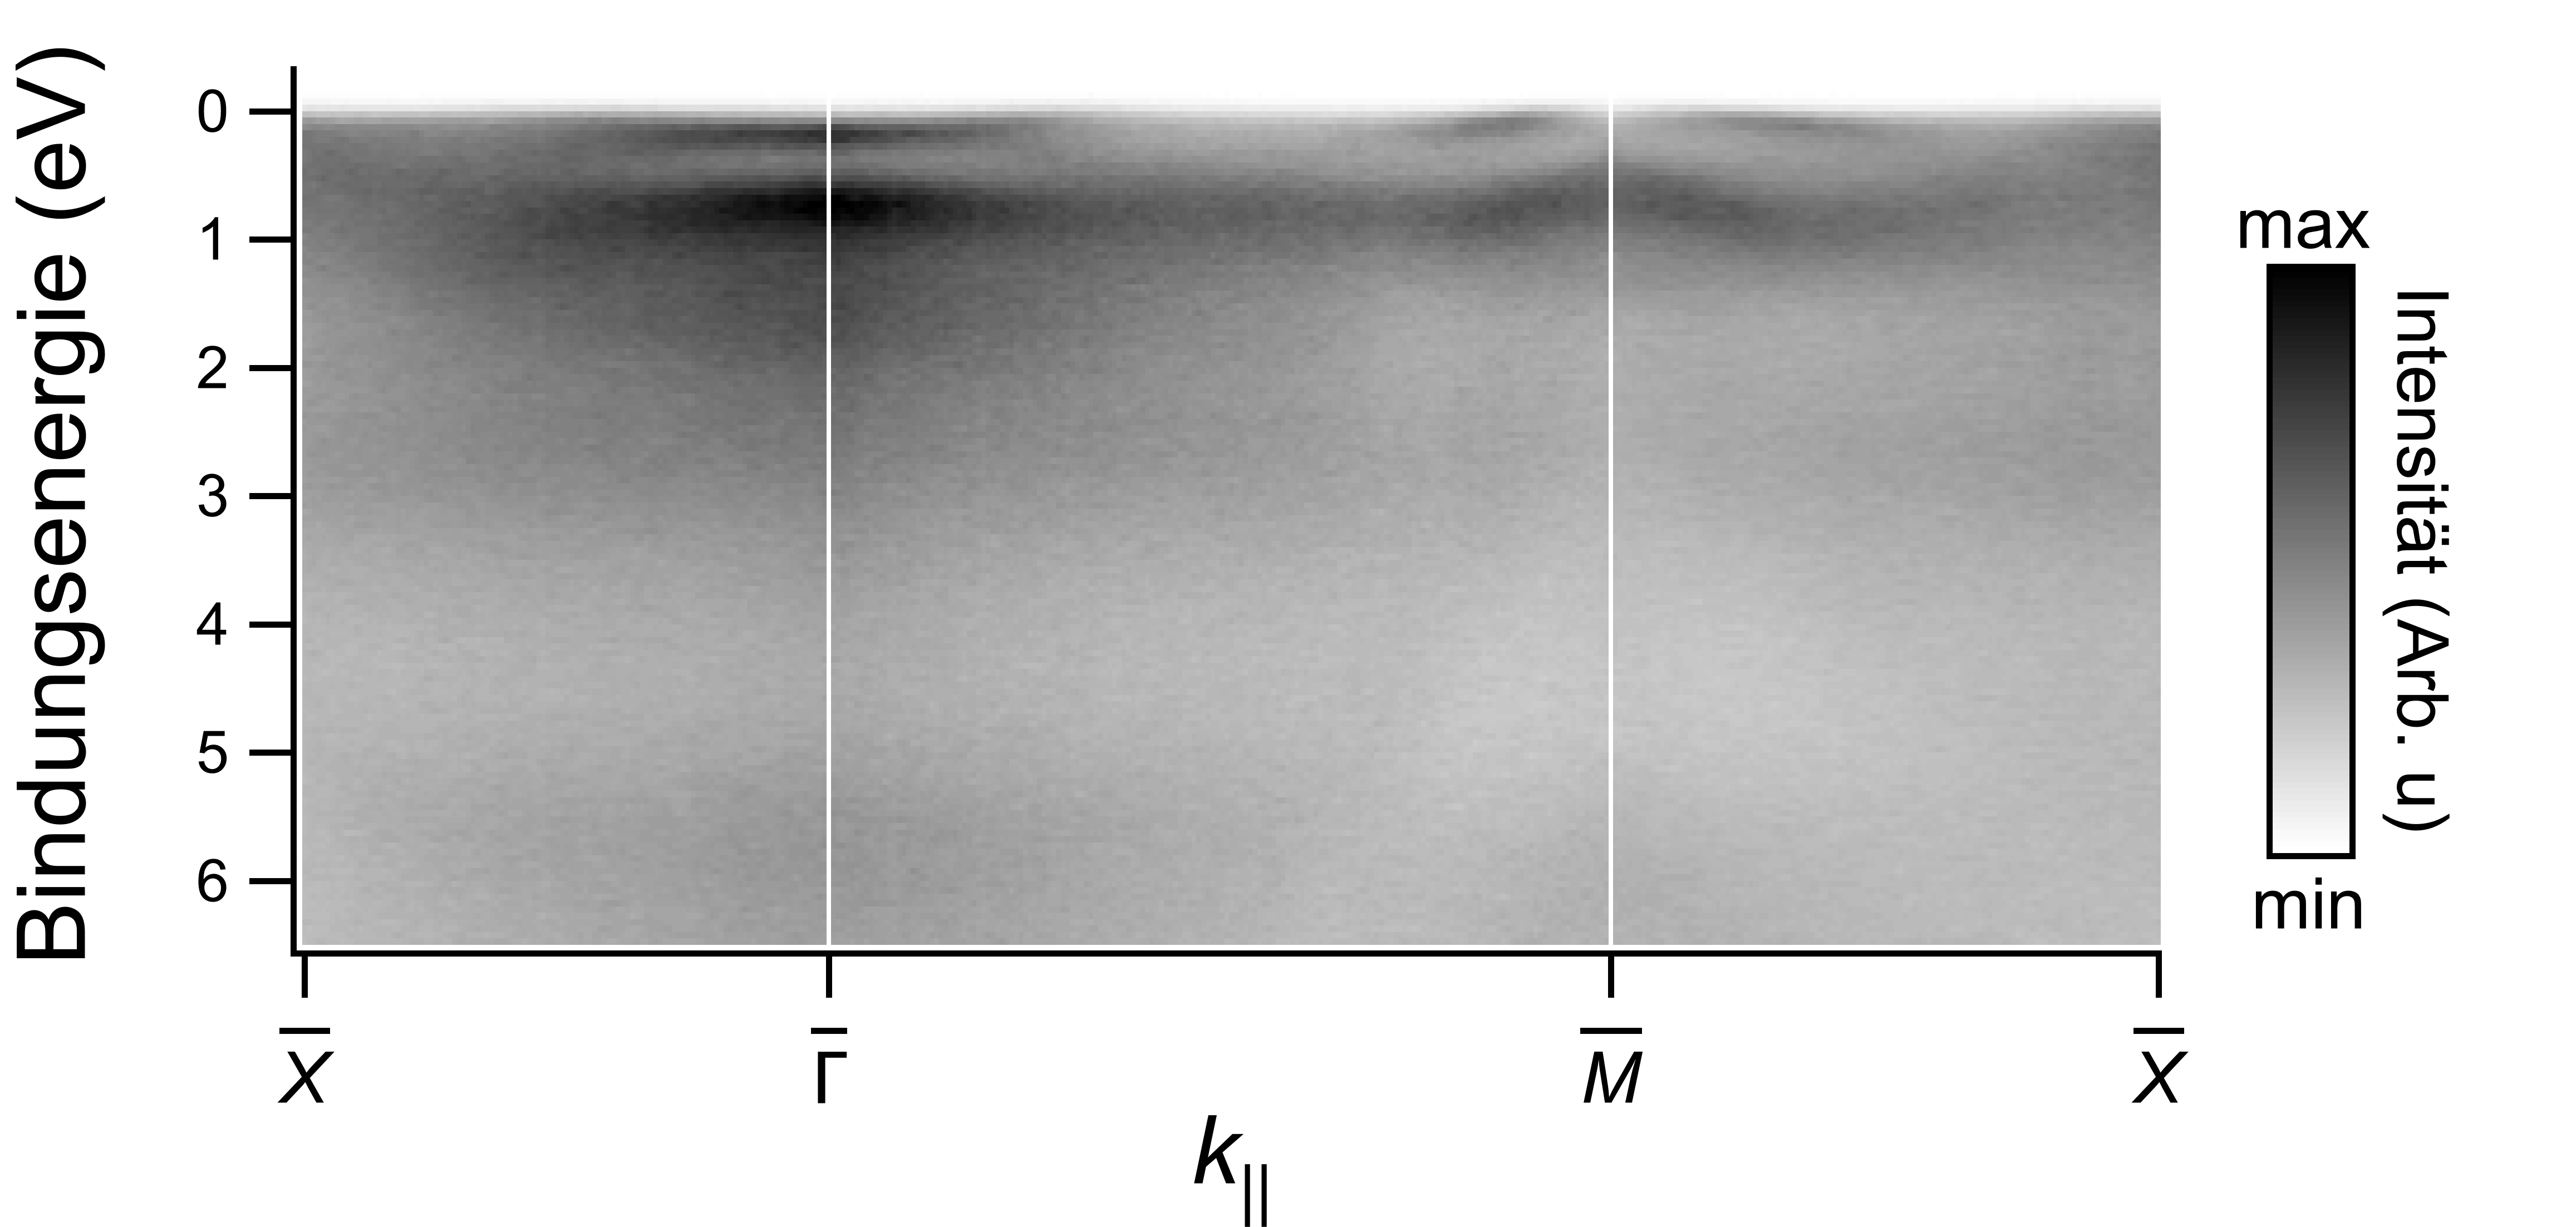
\includegraphics[height=4cm]{Fe/Band_Fe_2.png}
                \subcaption{}
                % Die Bandstruktur des reinen Eisens entlang einiger Hochsymmetrierichtungen.
                % Verwendete Photonenenergie war \SI{64}{\electronvolt} und die Polarisation p.
                \label{fig:Band_Fe}
            \end{subfigure}
            \caption{(\subref{fig:BZ_Fe}) Die erste Oberflächenbrillouinzone des Eisens (gelb), gemeinsam mit den Hochsymmetriepunkten. Das Bild ist bei einer Bindungsenergie von \SI{0.3}{\electronvolt} aufgenommen.
            (\subref{fig:Band_Fe}) Die entlang der grünen Linien in (\subref{fig:BZ_Fe}) extrahierte Bandstruktur der Eisen (100)-Oberfläche für eine Photonenenergie von \SI{64}{\electronvolt}.}
        \end{figure}
        Wie schon für das Gold lässt sich auch die Oberflächenbrillouinzone des Eisens darstellen. 
        Dies ist in \autoref{fig:BZ_Fe} geschehen.
        Aus ihr lässt sich anschließend die Bandstruktur extrahieren, welche in \autoref{fig:Band_Fe} abgebildet ist.
        Die Auflösung und Messstatistik lässt es allerdings nicht zu einzelne Bänder aufzulösen. %, auch wenn die winkelaufgelöste Messung in \autoref{fig:BZ_Fe} gut aufgelöst scheint. 
        Im oberen Bereich zwischen der Fermikante und etwa \SI{1}{\electronvolt} ist eine erhöhte Intensität zu vernehmen, welche durch die d-Bänder des Eisens hervorgerufen wird.        

        \begin{figure}
            \centering
            \begin{subfigure}[t]{0.48\textwidth}
                \centering
                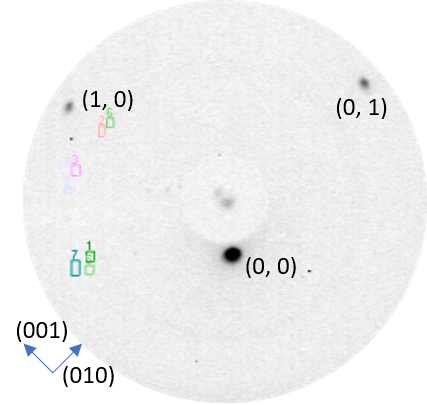
\includegraphics[height=5cm]{pFe/2021_09_07_001_passivatedFe(100)_44eV_mod.png}
                \subcaption{}
                \label{fig:LEED_pFe_44}
            \end{subfigure}
            \begin{subfigure}[t]{0.48\textwidth}
                \centering
                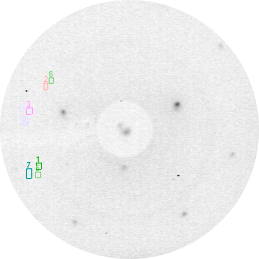
\includegraphics[height=5cm]{pFe/2021_09_07_002_passivatedFe(100)_125eV.png}
                \subcaption{}
                \label{fig:LEED_pFe_125}
            \end{subfigure}
            \caption{Beugungsbild der niederenergetischen Elektronen der passivierten Eisen (100)-Oberfläche bei einer Elektronenenergie von \SI{44}{\electronvolt} (\subref{fig:LEED_pFe_44}) und \SI{125}{\electronvolt} (\subref{fig:LEED_pFe_125}).}
            \label{fig:LEED_pFe}
        \end{figure}        
        Um Verunreinigungen des sehr reaktiven sauberen Eisens nach der Reinigung zu vermeiden, wird die Probe anschließend direkt passiviert.
        Dies geschieht in einer Sauerstoffatmosphäre von \SI{1.3e-7}{\milli\bar} für fünf Minuten, während die Probe bei \SI{550}{\celsius} gehalten wird.
        Anschließend wird die Probe kurz auf \SI{600}{\celsius} aufgeheizt.
        Die resultierenden LEED-Bilder sind in \autoref{fig:LEED_pFe} zu sehen.
        Die Beugungsreflexe sind scharf und zeigen die Geometrie der $\ce{Fe}-\text{p}(1 \times 1)\ce{O}$ Überstruktur.
        Alle Reflexe sind dabei nicht zentrosymmetrisch, da die Probe verkippt ist, wodurch der $(0, 0)$-Reflex zu sehen ist.

        Auf die passivierte Eisenoberfläche wird Eisen mit einer Rate von \SI{0.6}{\ML\per\minute} und einem Sauerstoffdruck von \SI{2e-7}{\milli\bar} aufgedampft.
        Dabei wird die Probe auf eine Temperatur von \SI{230}{\celsius} gehalten.
        Zum Abschluss wird die Temperatur auf \SI{600}{\celsius} für fünf Minuten erhöht.
        \begin{figure}
            \begin{subfigure}[t]{0.48\textwidth}
                \centering
                \includegraphics[height=5cm]{Fe3O4/2021_09_07_012_FeO(100)_44eV_Super.pdf}
                \subcaption{}
                \label{fig:LEED_Fe3O4}
            \end{subfigure}
            \begin{subfigure}[t]{0.48\textwidth}
                \centering
                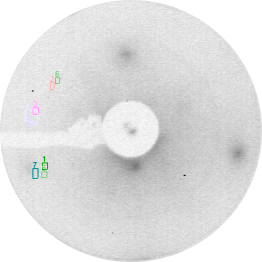
\includegraphics[height=5cm]{FeO/2021_09_09_001_FeO_125eV.png}
                \subcaption{}
                \label{fig:LEED_FeO}
            \end{subfigure}
            \caption{Das Beugungsbild der Oberfläche nach dem Aufdampfen von Eisen in einer Sauerstoffatmosphäre bei einer Elektronenenergie von \SI{44}{\electronvolt} (\subref{fig:LEED_Fe3O4}).
            Ebenfalls eigenzeichnet sind die Reflexe des Substrates (blau) und die der Überstruktur (rot, erstellt mit \cite{SpotPlotter}), sowie das Beugungsbild der modifizierten Oberfläche bei einer Elektronenenergie von \SI{125}{\electronvolt} (\subref{fig:LEED_FeO}).}
        \end{figure}
        So ergibt sich das Beugungsbild der Oberfläche in \autoref{fig:LEED_Fe3O4}.
        Aus der Position der Reflexe lässt sich eine $2\left(\sqrt{2}\times\sqrt{2}\right)$R\SI{45}{\degree}-Überstruktur rekonstruieren.
        Für eine Kristallterminierte Oberfläche, wird aufgrund der etwa doppelt so großen Einheitszelle des Magentits im Vergleich zum passivierten Eisen eine p$(2\times2)$-Überstruktur erwartet~\cite{FeO_1}.
        Aus der Literatur ist bekannt, dass sich bei einer reinen \ce{Fe3O4}(100) Oberfläche auch eine $\left(\sqrt{2}\times\sqrt{2}\right)\text{R}\SI{45}{\degree}$-Rekonstruktion ergeben könnte~\cite{ruwisch_vsm-untersuchung_2016}.
        Beides ist hier nicht zu erkennen, es hat sich also keine bekannte \ce{Fe3O4}(100) Oberflächenrekonstruktion ausgebildet.
        % Auch Gitterverzerrungen aus den ersten Lagen können zu Verzerrungen führen, wird für die verwendete Schichtdicke aber nicht mehr erwartet und es sollte wieder der ursprünglichen Gitterkonstante entsprechen.

        Um die Wüstitstruktur zu erhalten wird der aufgedampfte Film zunächst auf \SI{650}{\celsius} aufgeheizt.
        Anschließend werden vermehrt Sauerstoffatome durch ioneninduziertes Zerstäuben ausgelöst~\cite{FeO_36}.
        Im Anschluss wird die Probe nochmal auf \SI{650}{\celsius} erwärmt um die Fehlstellen auszuheilen.
        Dies sollte unabhängig von dem vorherrschenden Eisenoxid zu dem gewünschten Wüstit führen~\cite{FeO_12, FeO_15}.
        Welches in dem LEED Bild aus \autoref{fig:LEED_FeO} zu erkennen ist.
        Die Intensitäten sind beim Eisenmonooxid im Gegensatz zu dem passivierten Eisen invertiert, wobei die zuvor starken Reflexe nicht mehr sichtbar sind.
        Trotz der gleichen Elektronenenergie von \SI{125}{\electronvolt} sind die Punkte leicht nach außen gewandert.
        Dies widerspricht sich mit der eigentlich größeren Gitterkonstante vom Eisenmonooxid im Bezug auf die $\text{p}(1 \times 1)\ce{O}$-Überstruktur des passivierten Eisens, wodurch die Reflexe in Richtung des Zentrums wandern sollten.
        Zusätzlich erscheinen die einzelnen Punkte recht ausgewaschen, was auf Unregelmäßigkeiten in der Oberfläche deutet.
        Ein klarer Unterschied ist zu dem frisch aufgedampften Film in \autoref{fig:LEED_Fe3O4} zu sehen.
        Die Effekte der $2\left(\sqrt{2}\times\sqrt{2}\right)$R\SI{45}{\degree}-Überstruktur sind verschwunden. % und es ergibt sich die erwartete Intensitätsverteilung.

        \begin{figure}
            \centering
            \begin{subfigure}[t]{0.48\textwidth}
                \centering
                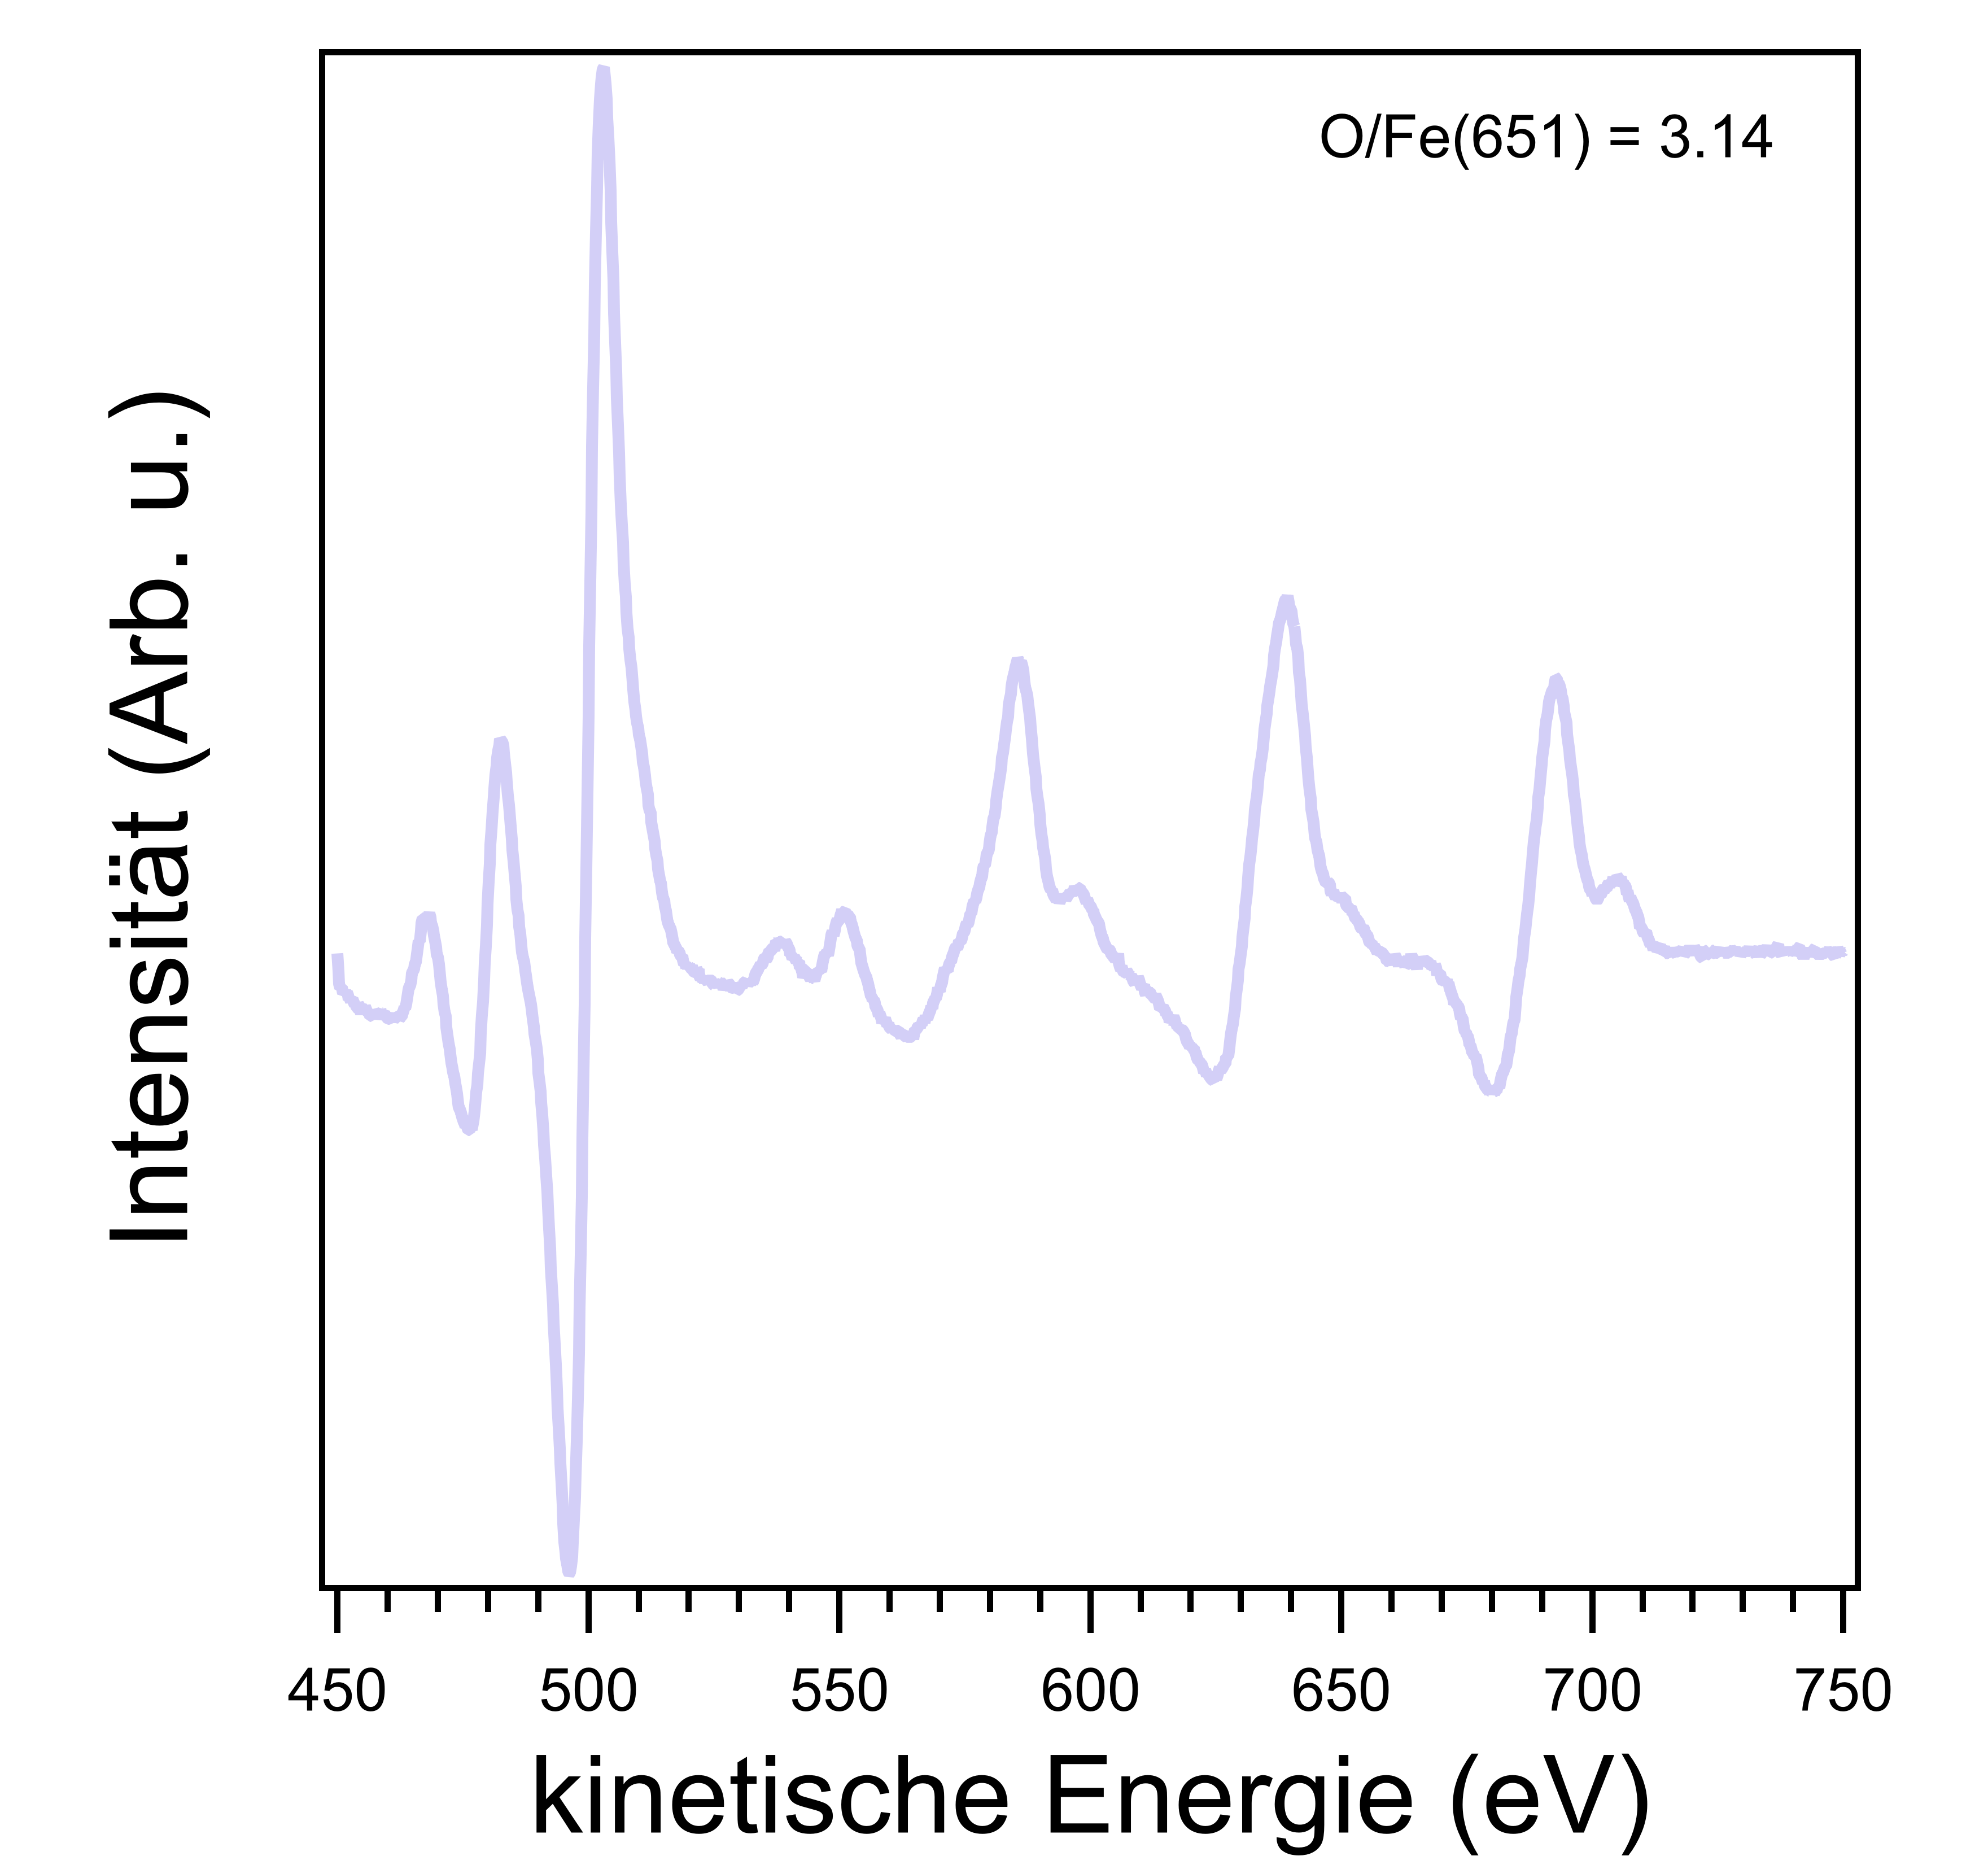
\includegraphics[height=6cm]{Fe3O4/AES_Fe3O4.png}
                \subcaption{}
                \label{fig:Auger_Fe3O4}
            \end{subfigure}
            \begin{subfigure}[t]{0.48\textwidth}
                \centering
                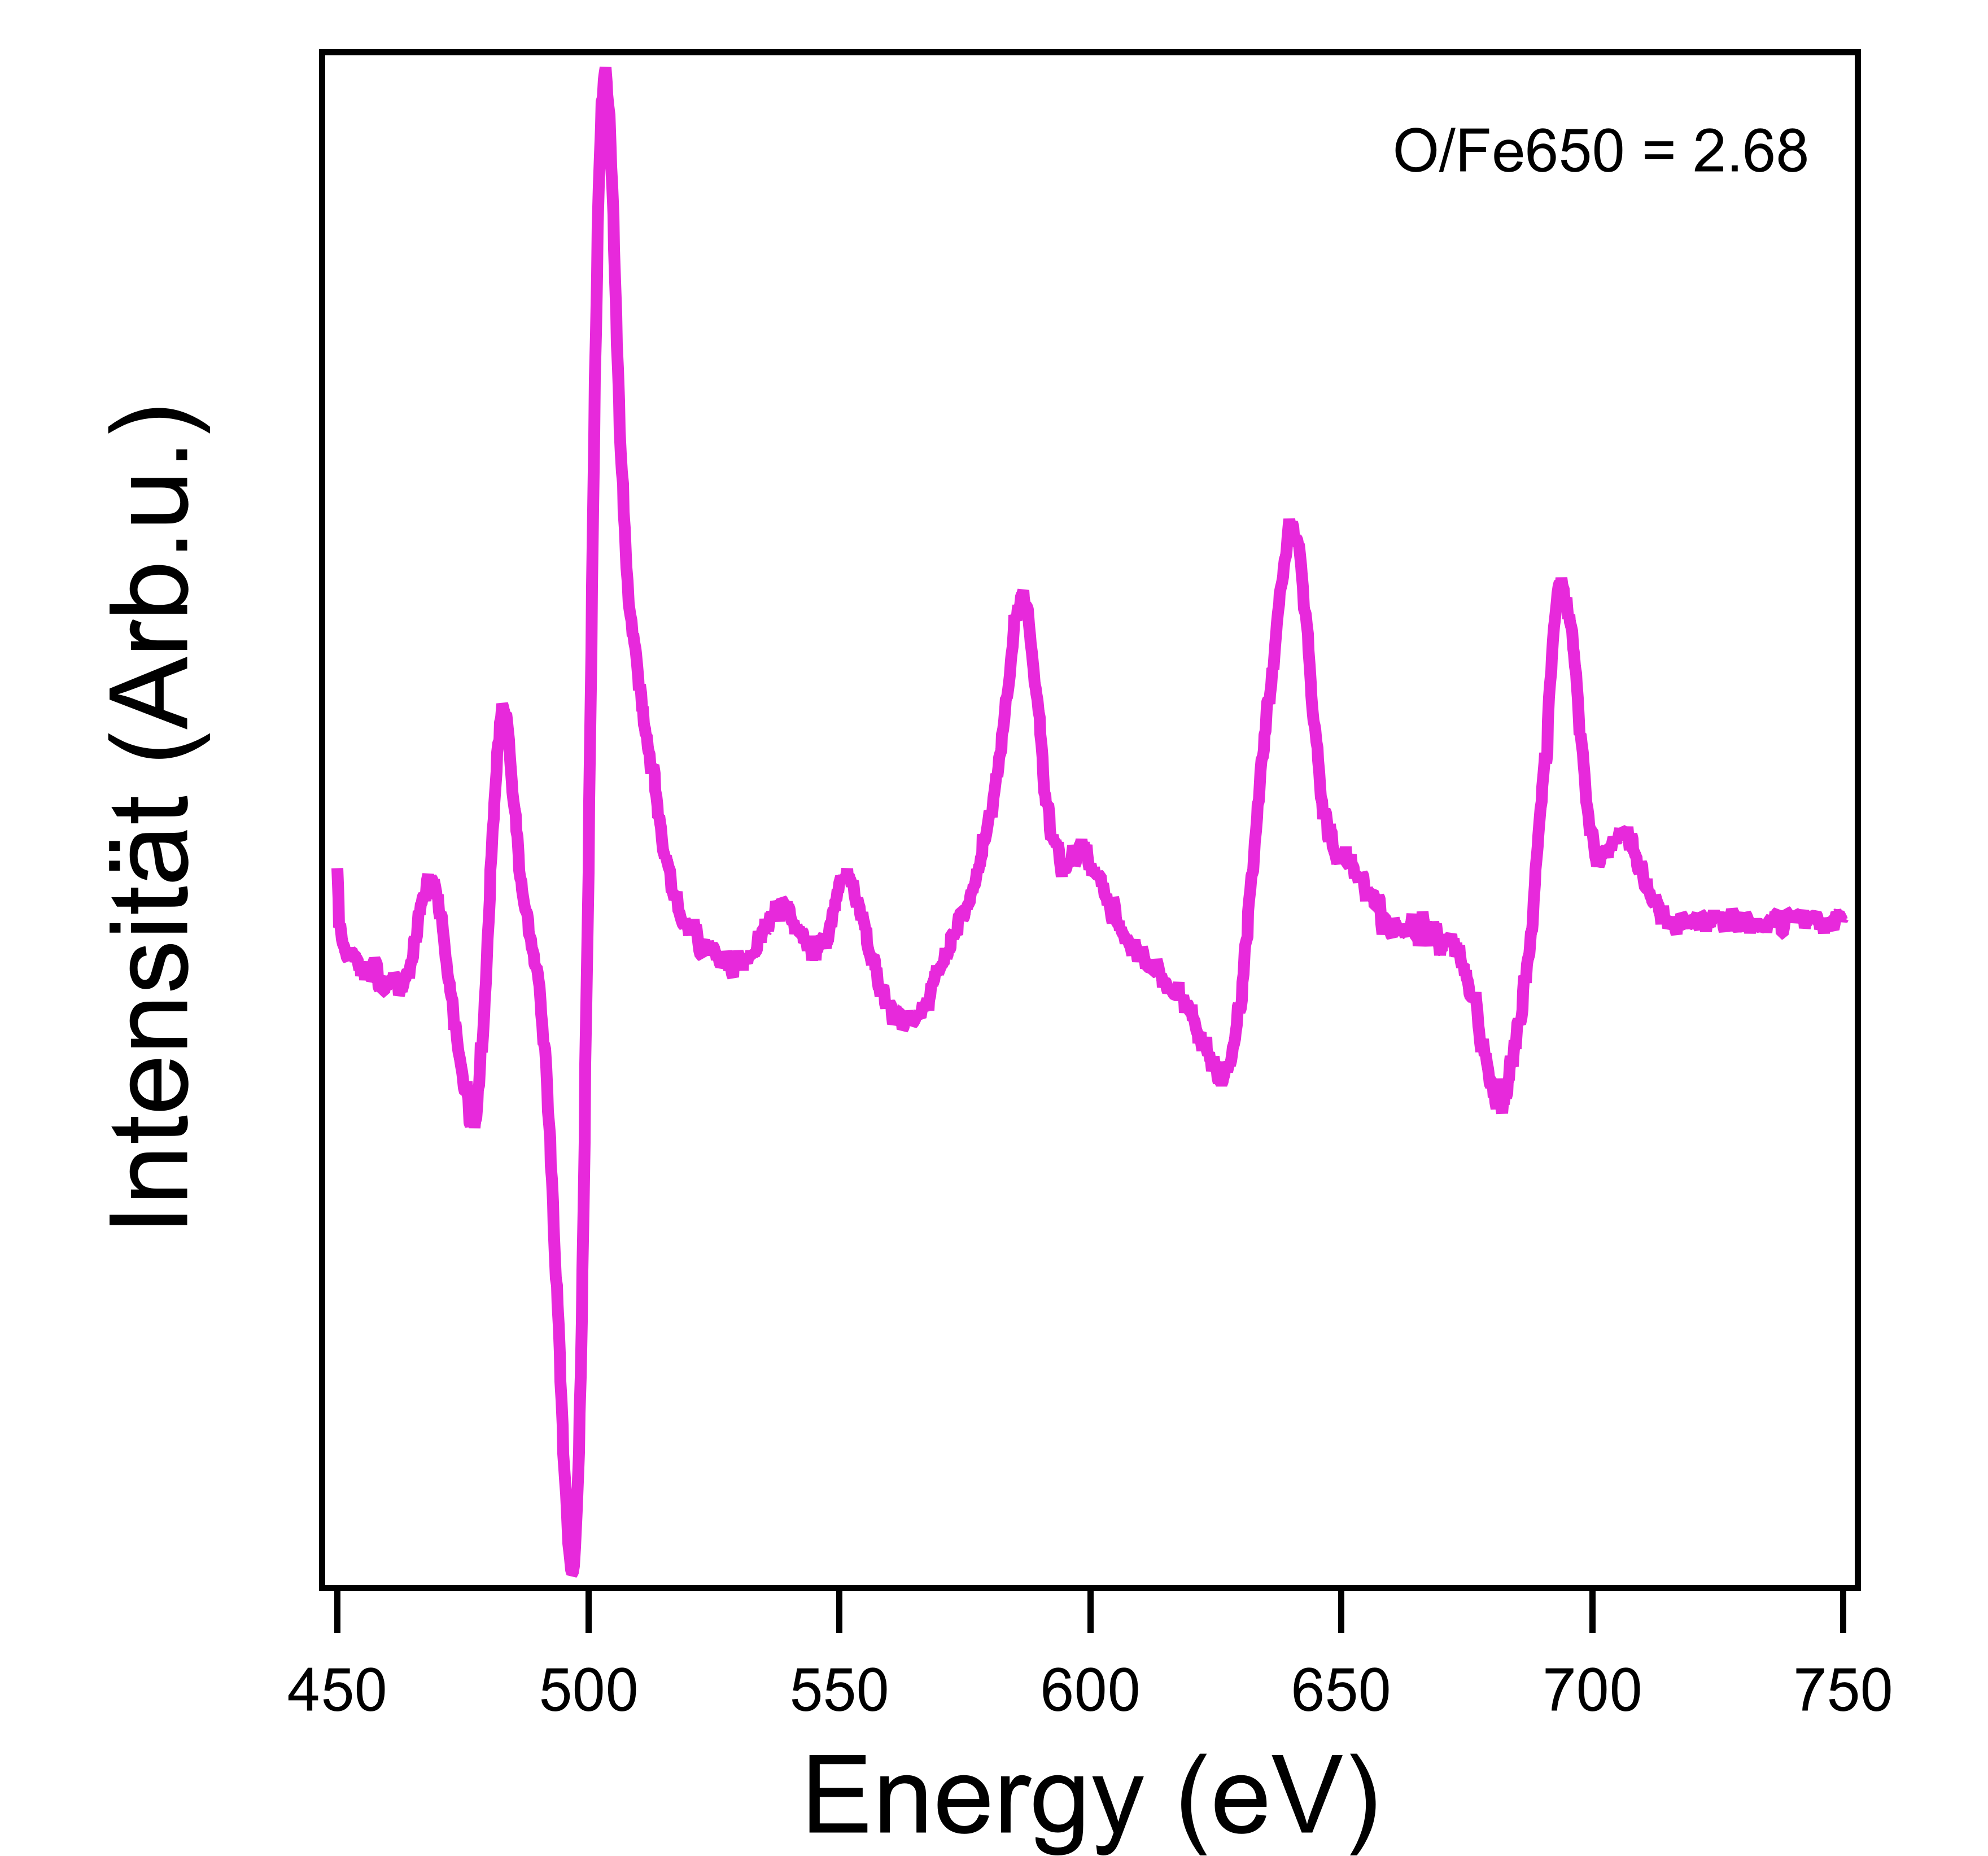
\includegraphics[height=6cm]{FeO/AES_FeO.png}
                \subcaption{}
                \label{fig:Auger_FeO}
            \end{subfigure}
            \caption{Die Augerspektren für den aufgedampften Film (\subref{fig:Auger_Fe3O4}) und den modifizierten Film (\subref{fig:Auger_FeO}).}
            \label{fig:Auger}
        \end{figure}
        Die Konzentrationen an Sauerstoff und Eisen werden in beiden Filmen mittels Augerelektronenspektroskopie analysiert.
        So ergibt sich das Augerspektrum in \autoref{fig:Auger_Fe3O4} für den frisch aufgedampften Film.
        Hierbei kann das Signal bei \SI{503}{\electronvolt} dem KLL-Übergang des Sauerstoffs und dem LMM-Übergang des Eisens die Signale bei \SI{598}{\electronvolt}, \SI{651}{\electronvolt} und \SI{703}{\electronvolt} zugeordnet werden~\cite{Auger}. 
        Die drei unterschiedlichen Energien für das Eisen tauchen durch die Spin-Bahn-Aufspaltung des Eisens auf.
        Das Spitzenverhältnis zwischen dem Sauerstoffsignal bei \SI{503}{\electronvolt} und dem Signal für Eisen bei \SI{651}{\electronvolt} liefert ein Verhältnis von ca. \num{3.14}.
        Aus der Literatur ist bekannt das für Magnetit ein Wert von \num{3.86} erwartet wird~\cite{FeO_1}.
        Der ermittelte Wert weicht dabei nach unten ab, was durch das zusätzliche Aufheizen auf \SI{600}{\celsius} erklärt werden könnte.
        Dabei kommt es zur Umstrukturierung der Oberfläche und in Folge dessen zur Diffusion von Sauerstoff in Richtung des Substrates~\cite{FeO_62}.

        Wird das Verhältnis der Intensitäten der Signale bei \SI{503}{\electronvolt} und \SI{703}{\electronvolt} unter Beachtung der elementspezifischen Sensitivität ausgewertet, ergibt sich das stöchiometrischen Verhältnis.
        Die Sensitivität für Sauerstoff und Eisen unter der Verwendung von \SI{3}{\kilo\electronvolt} Primärelektronen liegt bei \num{0.5} respektive \num{0.2}~\cite{Auger}.
        % Damit lässt sich die Konzentration des Elements nach \autoref{eqn:Auger} bestimmen.
        Somit ergibt sich für die Konzentration von \ce{O}- und \ce{Fe}-Atomen ein Verhältnis von $\num{0.55}:\num{0.45}$.
        Dieses Verhältnis weicht nur leicht vom erwarteten Verhältnis $\num{0.57}:\num{0.43}$ ab.
        Auf Grund der Dicke des Films von etwa \SI{45}{\angstrom} ist ein Beitrag durch das Eisen-Substrat zu vernachlässigen.
        % Problem bereitet natürlich das Substrat, was ebenfalls aus Eisen besteht und auch die passivierte Schicht enthält bereits Sauerstoff.

        Für den modifizierten Film ergibt sich ein Verhältnis zwischen dem Sauerstoffsignal bei \SI{503}{\electronvolt} und dem Signal für Eisen bei \SI{651}{\electronvolt} von \num{2.68} ausdem in \autoref{fig:Auger_FeO} abgebildetem Spektrum.
        Dies deutet auf $\ce{FeO}$ hin, da dies nur leicht unterhalb des Wertes aus der Literatur von \num{2.89} liegt~\cite{FeO_1}.
        Die kleine Abweichung nach unten kann dadurch erklärt werden, dass es sich um einen sehr dünnen Film auf Eisen handelt, der durch das ioneninduzierte Zerstäuben entstanden ist.
        Die Augerelektronen mit ihrer für Eisen typischen kinetischen Energie weisen eine inelastische mittlere freie Weglänge von etwa \SI{14}{\angstrom} auf.
        Hierdurch ist die Oberflächensensitivität nicht mehr gegeben und es könnte einen Beitrag durch das Eisensubstrat geben.
        In Folge dessen würde sich das relative Verhältnis reduzieren.
        Ebenso zeigt das Augerspektrum mit dem bereits von Carpa u.A.~\cite{FeO_1} entdecken Augerelektronenspektrum für Eisenmonooxid gute Übereinstimmung.

        \begin{figure}
            \begin{subfigure}[t]{0.48\textwidth}
                \centering
                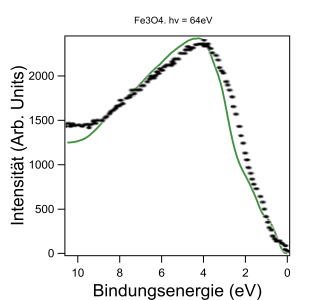
\includegraphics[height=5.5cm]{Fe3O4/VB_Fe3O4.png}
                \subcaption{}
                \label{fig:EDC_Fe3O4}
            \end{subfigure}
            \begin{subfigure}[t]{0.48\textwidth}
                \centering
                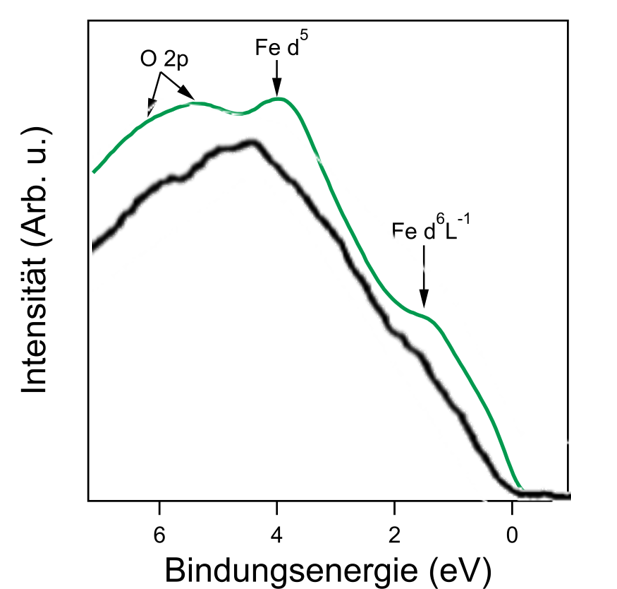
\includegraphics[height=5.5cm]{FeO/VB_FeO_2.png}
                \subcaption{}
                \label{fig:EDC_FeO}
            \end{subfigure}
            \caption{Die Valenzbandspektren (grün) bei einer Photonenenergie von \SI{64}{\electronvolt} und p Polarisation für den aufgedampften Film (\subref{fig:EDC_Fe3O4}) und des behandelten Films (\subref{fig:EDC_FeO}).
            Ebenso sind jeweils Referenzmessungen aus der Literatur in schwarz eingetragen.
            Diese stammen für (\subref{fig:EDC_Fe3O4}) aus \cite{FeO_35} und wurde bei einer Photonenenergie von \SI{59}{\electronvolt} aufgenommen.
            Für (\subref{fig:EDC_FeO}) wurde ein Photonenenergie von \SI{65}{\electronvolt} verwendet und entstammt aus \cite{FeO_14}.
            Zusätzlich sind die identifizierten Merkmale eingetragen.}
            \label{fig:EDCs}
        \end{figure}
        Bei der Betrachtung der Valenzbandspektren in \autoref{fig:EDCs} fallen deutliche Unterschiede auf.     
        Ein Vergleich zwischen dem winkelintegrierte Spektrum des Valenzbands des aufgedampften Films in \autoref{fig:EDC_Fe3O4} (grün) zeigt gute Übereinstimmung mit der Literatur die durch schwarze Punkte angedeutet ist~\cite{FeO_35}.
        % Die kleine relative Verschiebung bei den Spitzen kann durch die Evaluation der Fermikante herrühren.
        Zusammen mit dem Ende der Sekundärelektronen ergibt sich die Austrittsarbeit zu \SI{4.35}{\electronvolt}.
        Damit liegt diese deutlich unter dem erwarteten Wert von \SI{5.2}{\electronvolt}~\cite{FeO_40}.
        Besonders für Oxide kann die Austrittsarbeit deutlich vom Präparationsprozess und der Stöchiometrie abhängen, sodass ein Unterschied von einem Elektronenvolt keine Besonderheit darstellt~\cite{IF_11}.
        Das Valenzbandspektrum des modifizierten Films in \autoref{fig:EDC_FeO} (grün) zeigt im niederenergetischen Bereich recht gute Übereinstimmung mit der Literatur (schwarz)~\cite{FeO_14}.
        Bei größeren Bindungsenergien ist ein größerer Sauerstoffanteil zu erkennen.
        Denn das Spektrum lässt durch vier maßgebliche Beiträge beschreiben.
        Hierbei handelt es sich bei \SI{1.5}{\electronvolt} um den Beitrag des hybridisierten Zustand $\ce{Fe}\:\text{d}^6\text{L}^{-1}$ und bei \SI{4}{\electronvolt} um den Beitrag des $\ce{Fe}\:\text{d}^5$ Zustands~\cite{FeO_19}.
        Die Beiträge bei \SI{5.5}{\electronvolt}~\cite{FeO_44} und \SI{6.2}{\electronvolt}~\cite{FeO_18} haben ihren Ursprung bei den Sauerstoff 2p-Zuständen.
        Es ist dabei ein deutlicher Unterschied zu dem Spektrum des \ce{Fe3O4} in \autoref{fig:EDC_Fe3O4} zu erkennen.
        Beide Spektren zeigen eine recht ausgeprägte Spitze mit einer Schulter bei niedrigen Bindungsenergien.
        Mithilfe der Sekundärelektronen und der Fermikante lässt sich die Austrittsarbeit auf \SI{3.48}{\electronvolt} bestimmen.
        Dieser Wert passt damit zum Literaturwert von \SI{3.5}{\electronvolt}~\cite{FeO_28}.
        % Hinzu kommt bei einem dünnen Film die Austrittsarbeit auch maßgeblich von dem Übergang zwischen Metall und Oxid und dessen Defektstruktur abhängt~\cite{IF_10}.
        % Eine Absenkung der Austrittsarbeit kann dabei auf Sauerstofffehlstellen hindeuten~\cite{IF_11}, was ebenfalls durch das Augerspektrum bestätigt werden kann.
        
        \begin{figure}
            \centering
            \begin{subfigure}[t]{0.48\textwidth}
                \centering
                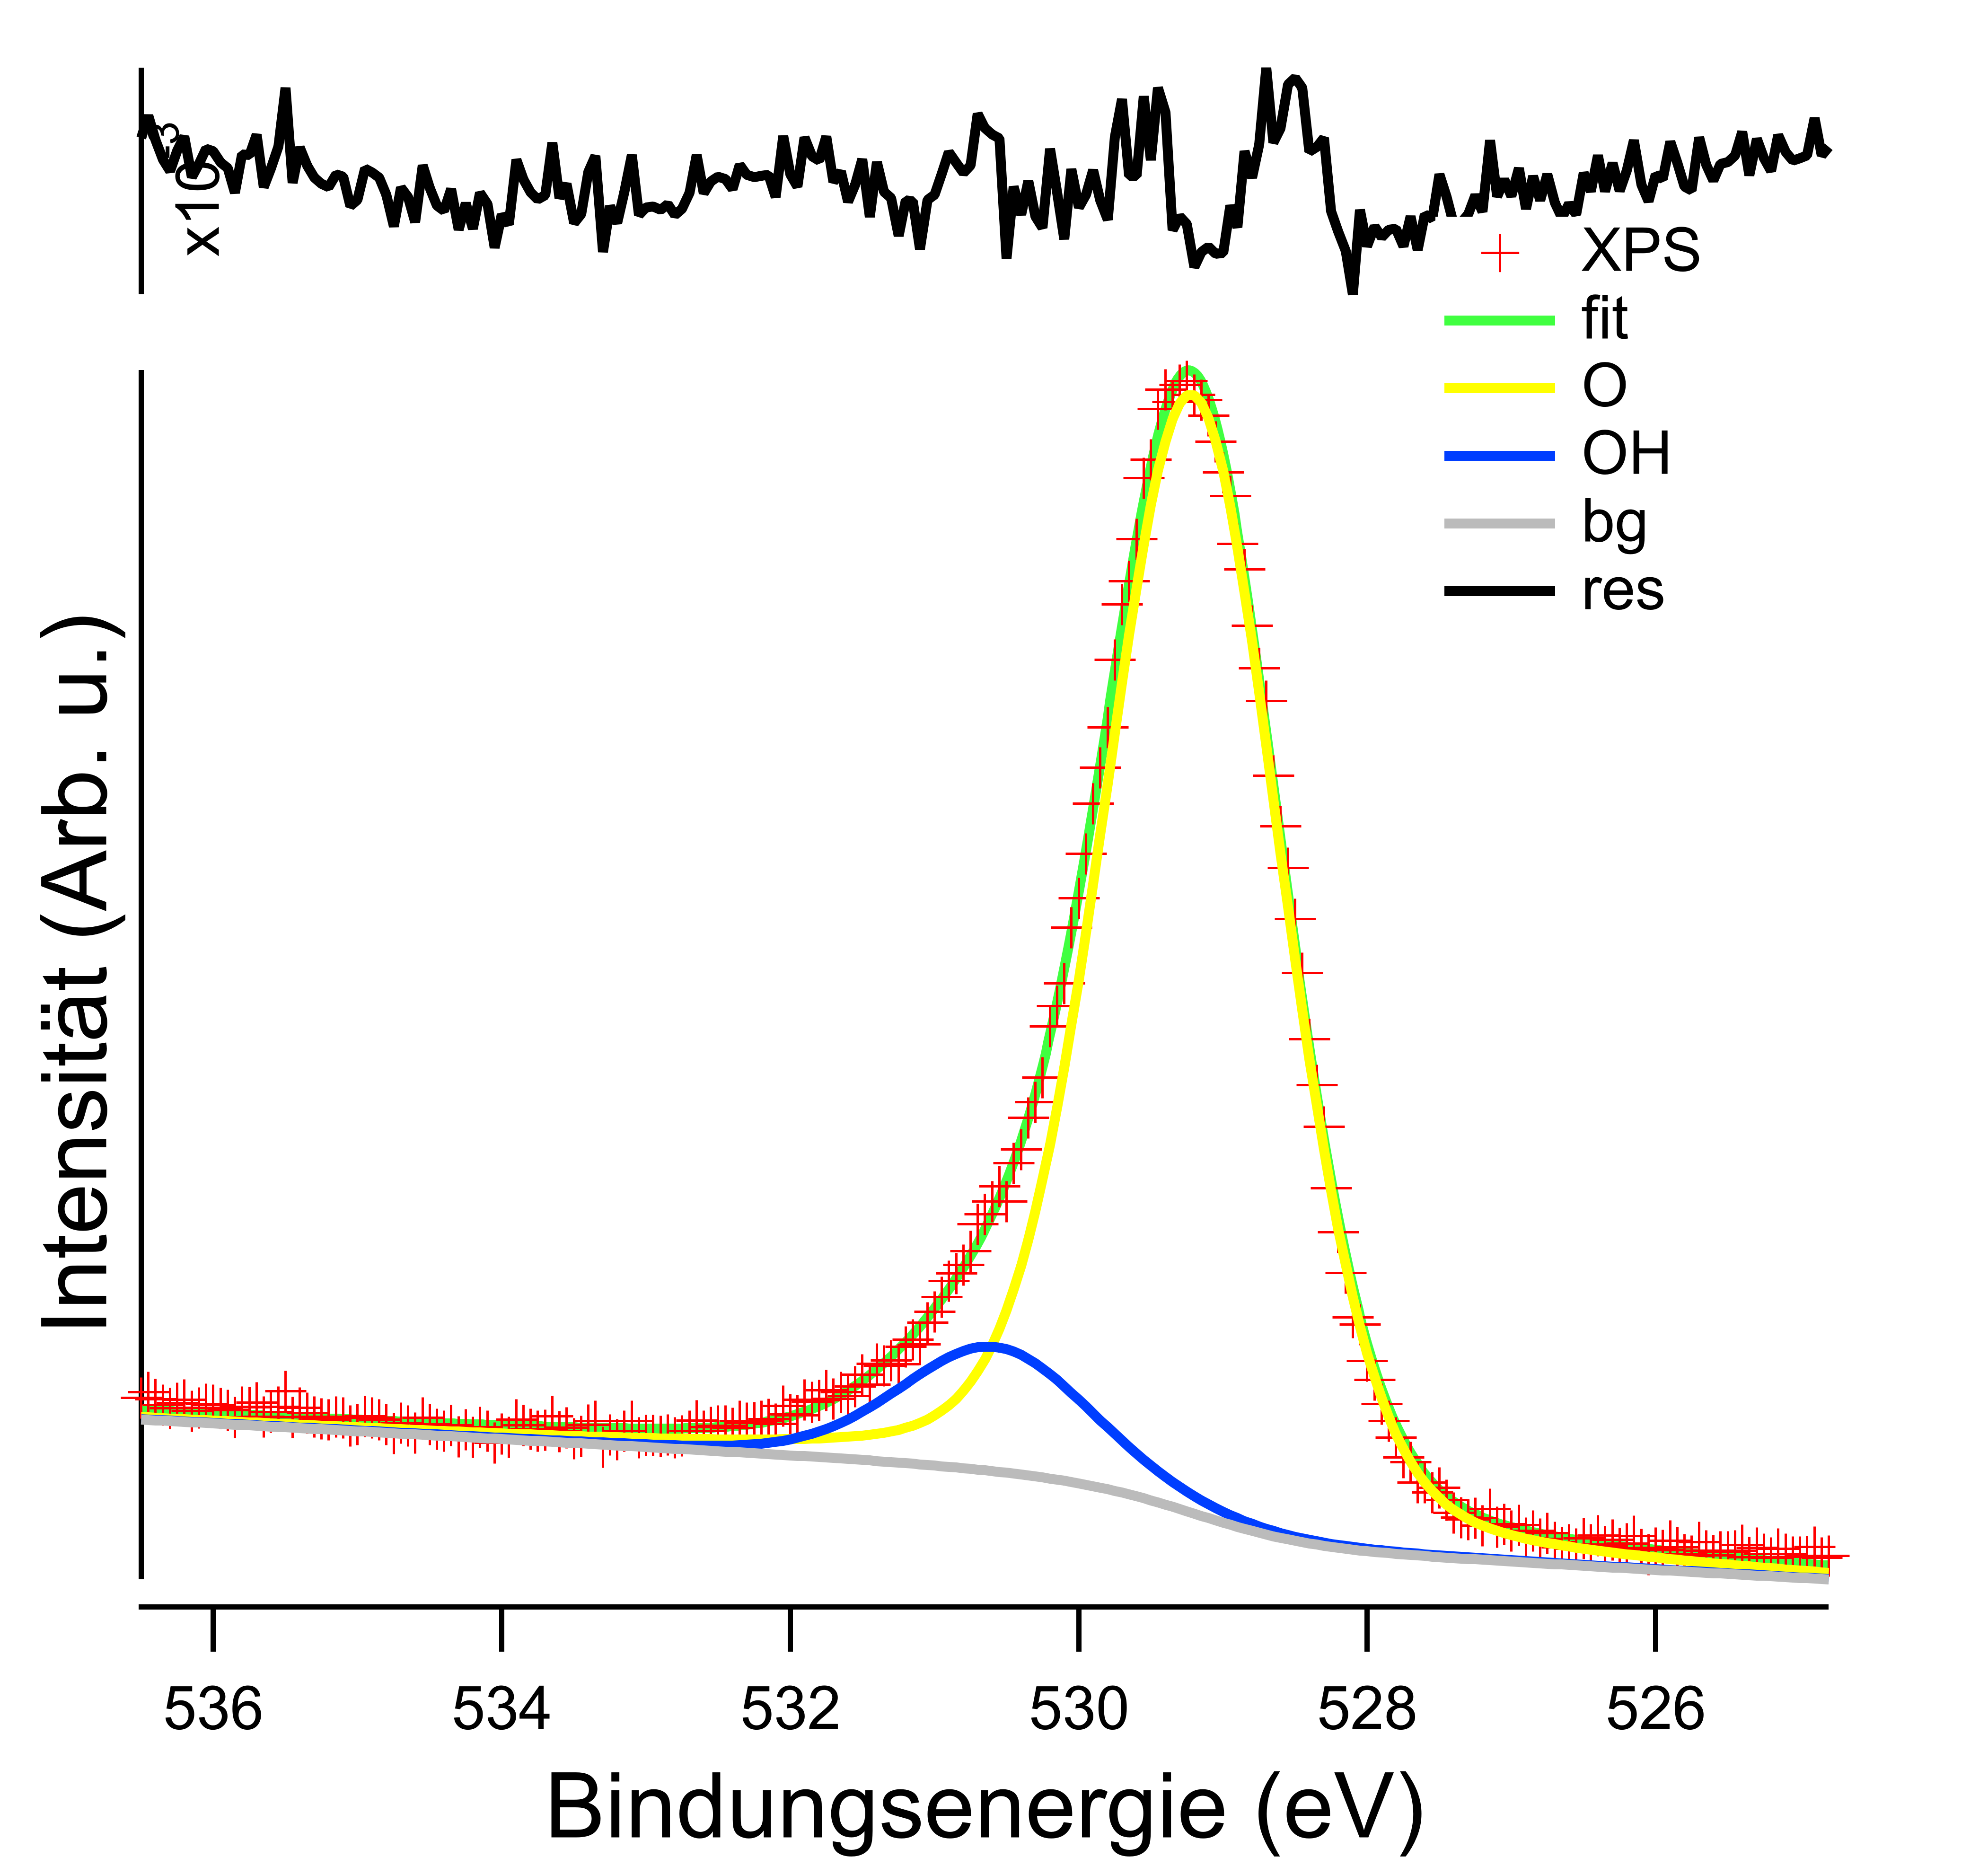
\includegraphics[height=6cm]{Fe3O4/O1s_Fe3O4.png}
                \subcaption{}
                \label{fig:XPSO1s_Fe3O4}
            \end{subfigure}
            \begin{subfigure}[t]{0.48\textwidth}
                \centering
                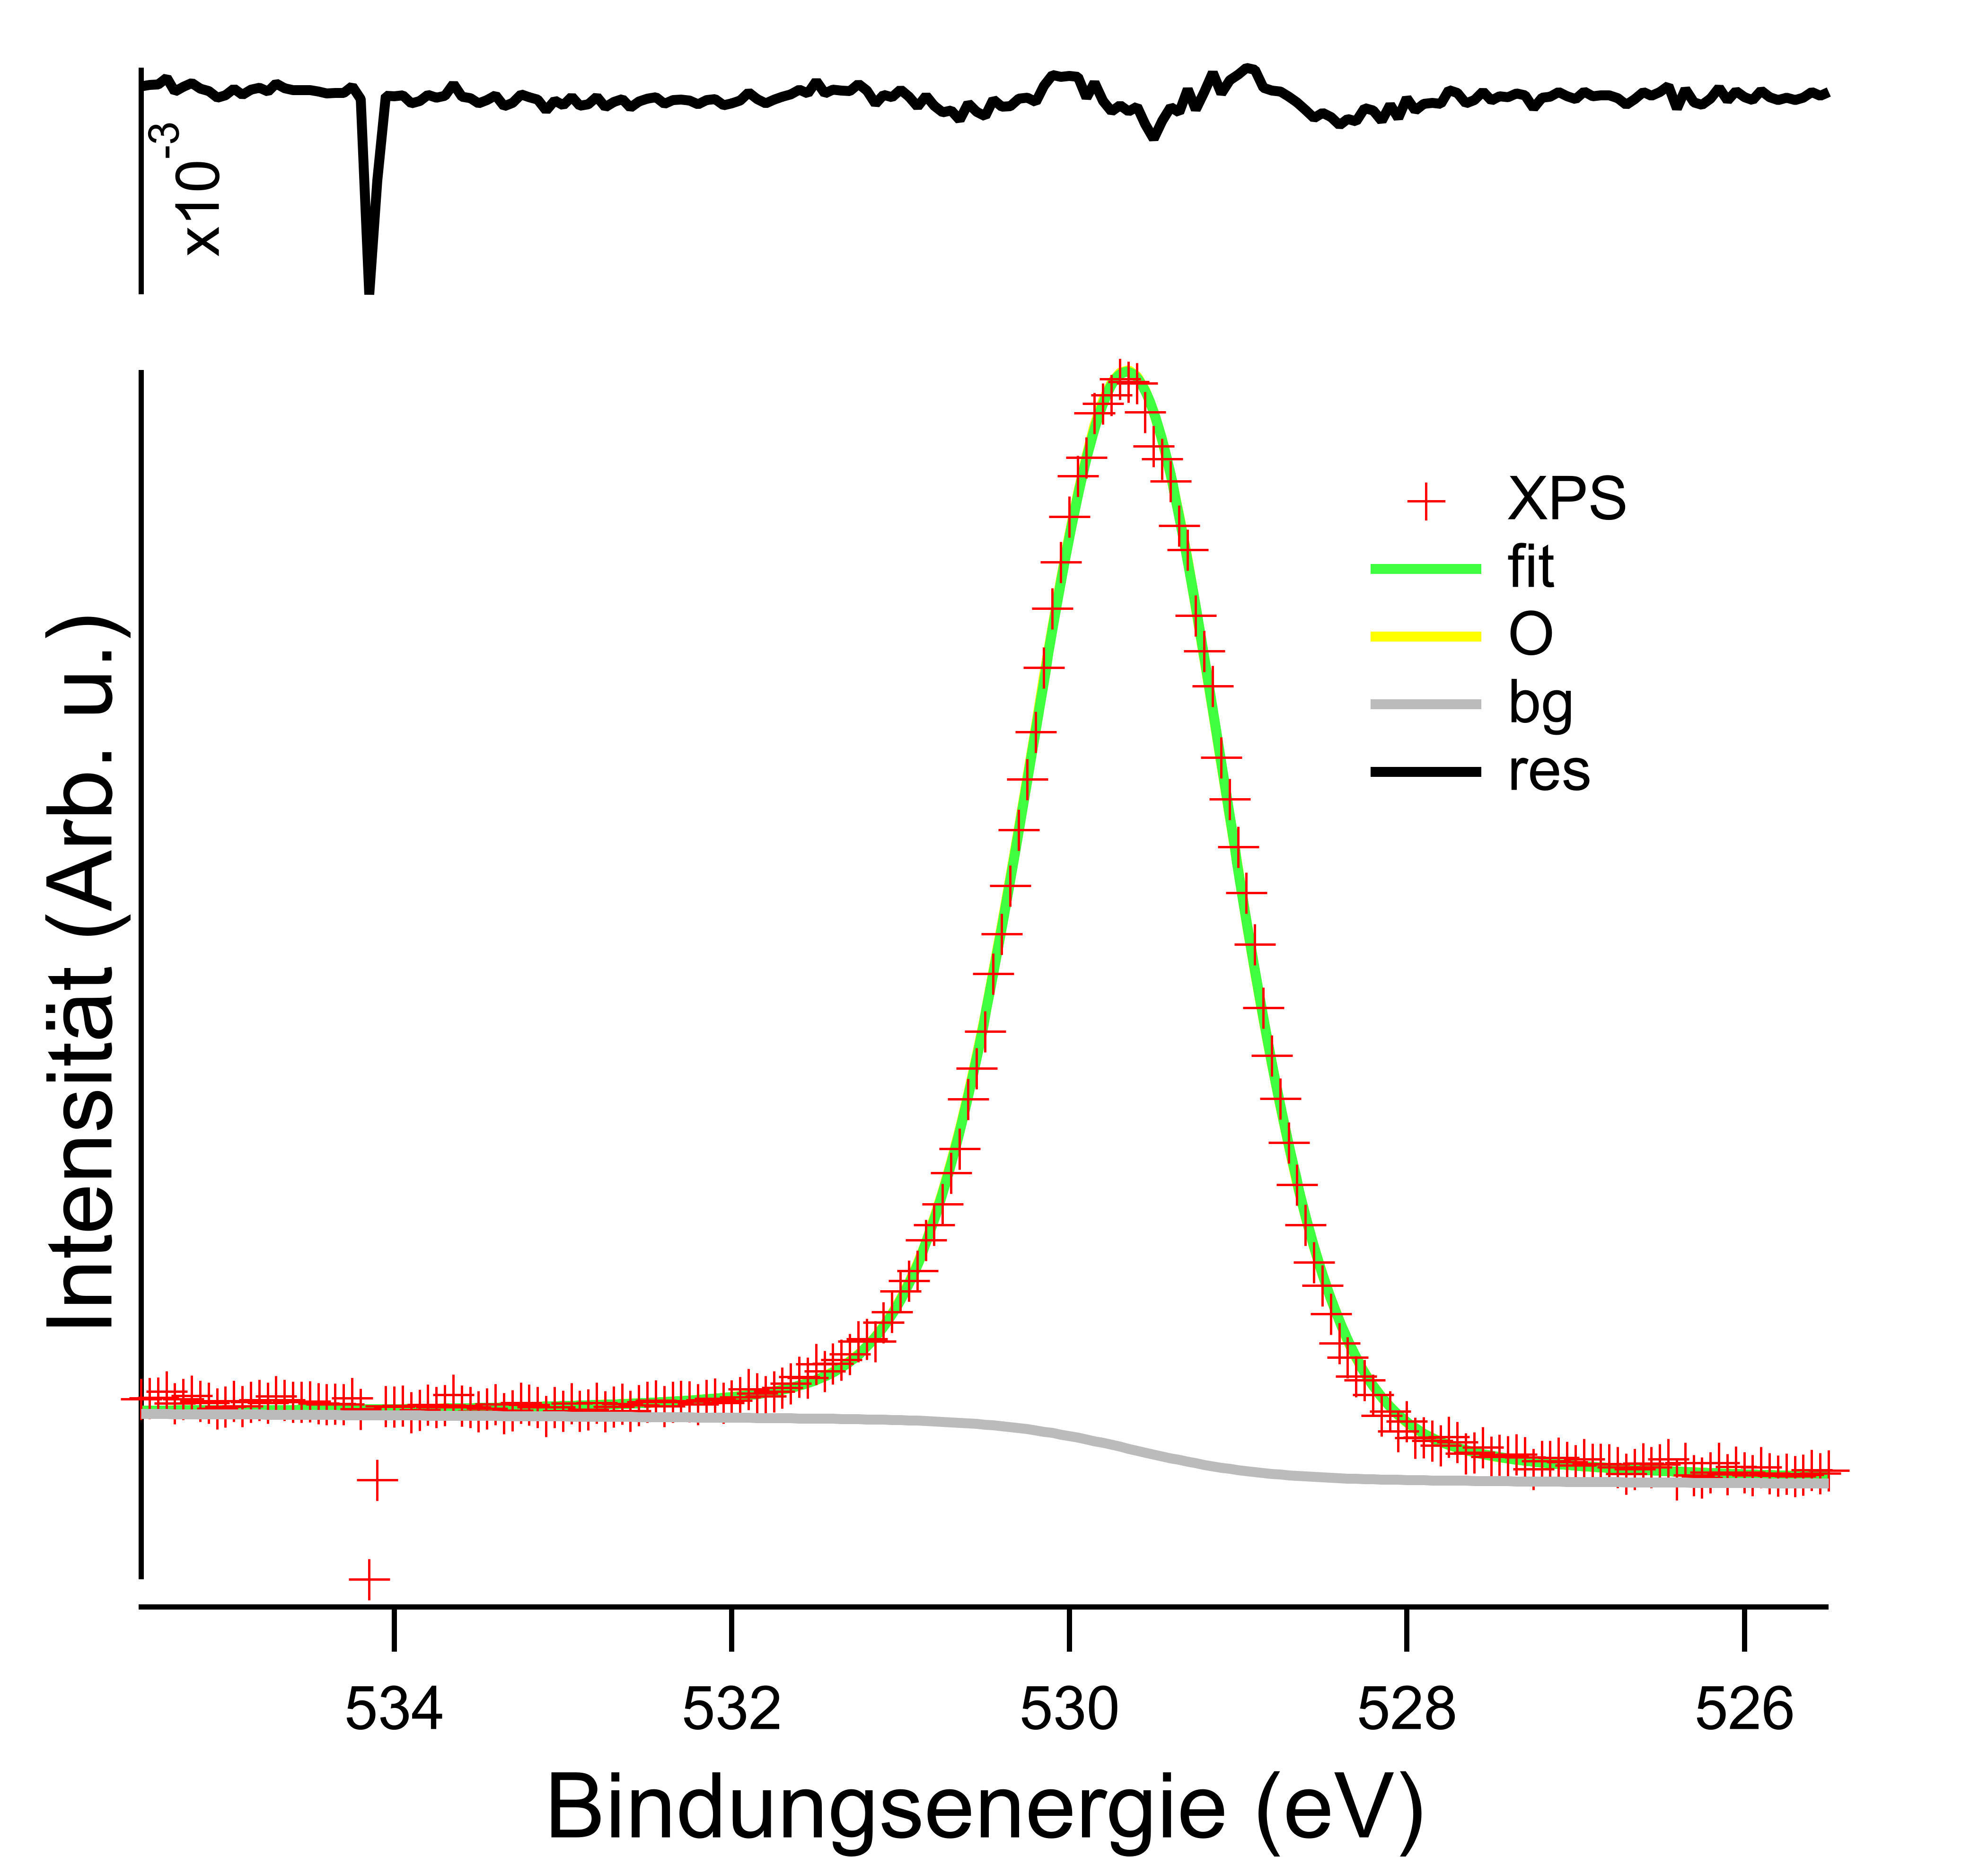
\includegraphics[height=6cm]{FeO/O1s_FeO.png}
                \subcaption{}
                \label{fig:XPSO1s_FeO}
            \end{subfigure}            
            \caption{Die XPS Spektren der beiden Filme des $\ce{O}_\text{1s}$-Niveaus wurde mit einer Photonenenergie von \SI{650}{\electronvolt} und s Polarisation aufgenommen.
            Links zu sehen in (\subref{fig:XPSO1s_Fe3O4}) ist der aufgedampfte Film und rechts in (\subref{fig:XPSO1s_FeO}) der modifizierte Film.}
            \label{fig:XPS_O1s}
        \end{figure}
        Um genauer die Zusammensetzung zu überprüfen werden XPS-Spektren aufgenommen.
        Die entsprechenden Spektren des $\ce{O}_{1\text{s}}$-Signals sind in \autoref{fig:XPS_O1s} dargestellt.
        Das $\ce{O}_{1\text{s}}$-Signal des aufgebrachten Films zeigt dabei einen kleinen Anteil einer \ce{OH}-Kontamination~\cite{FeO_9}.
        Aus der Position des $\ce{O}_{1\text{s}}$ lässt sich nach der Literatur keine Information über das vorhandene Eisenoxid gewinnen~\cite{FeO_15, FeO_9, FeO_64, wandelt_photoemission_1982}.
        Die Approximation wurde mittels zwei Pseudo-Voigt-Funktionen, sowie einem Shirley-Untergrund ermittelt~\cite{schmid_new_2014}.
        Für den Sauerstoffanteil liegt die ermittelte Position bei \SI{529.2}{\electronvolt} und damit unterhalb der erwarteten Position des Signals bei \SI{530.3}{\electronvolt}~\cite{wandelt_photoemission_1982}.
        Der \ce{OH}-Anteil liegt ebenfalls \SI{0.9}{\electronvolt} unterhalb des erwarteten Wertes von \SI{531.5}{\electronvolt}~\cite{wandelt_photoemission_1982}.
        Ursache könnte sein, dass es an einer Referenzmessung zur Bestimmung der Photonenenergie fehlt, welche mit \SI{650}{\electronvolt} angenommen wurde und damit zu einer konstanten Verschiebung führt.
        Die ermittelten Halbwertsbreiten hingegen passen recht gut zur Literatur von etwa \SI{1.6}{\electronvolt}~\cite{FeO_53} und sind mit \SI{1.5}{\electronvolt} sogar etwas kleiner.
        Beim modifizierten Film zeigt sich in \autoref{fig:XPSO1s_FeO} hingegen die Abwesenheit der \ce{OH}-Kontamination.
        Die Position lässt sich auf \SI{529.7}{\electronvolt} bestimmen und liegt wie schon für den direkt aufgebrachten Film leicht unterhalb des erwarteten Wertes.
        Da zwischen den beiden Messungen am Monochromator die Gitter getauscht wurden sind leichte unterschiedliche Photonenenergien anzunehmen.
        Dies würde deren relative Position der beiden Sauerstoff-Peaks von \SI{0.5}{\electronvolt} untereinander erklären, welcher nicht erwartet wird~\cite{FeO_15, FeO_9, FeO_64, wandelt_photoemission_1982}.

        \begin{figure}
            \centering
            \begin{subfigure}[t]{0.48\textwidth}
                \centering
                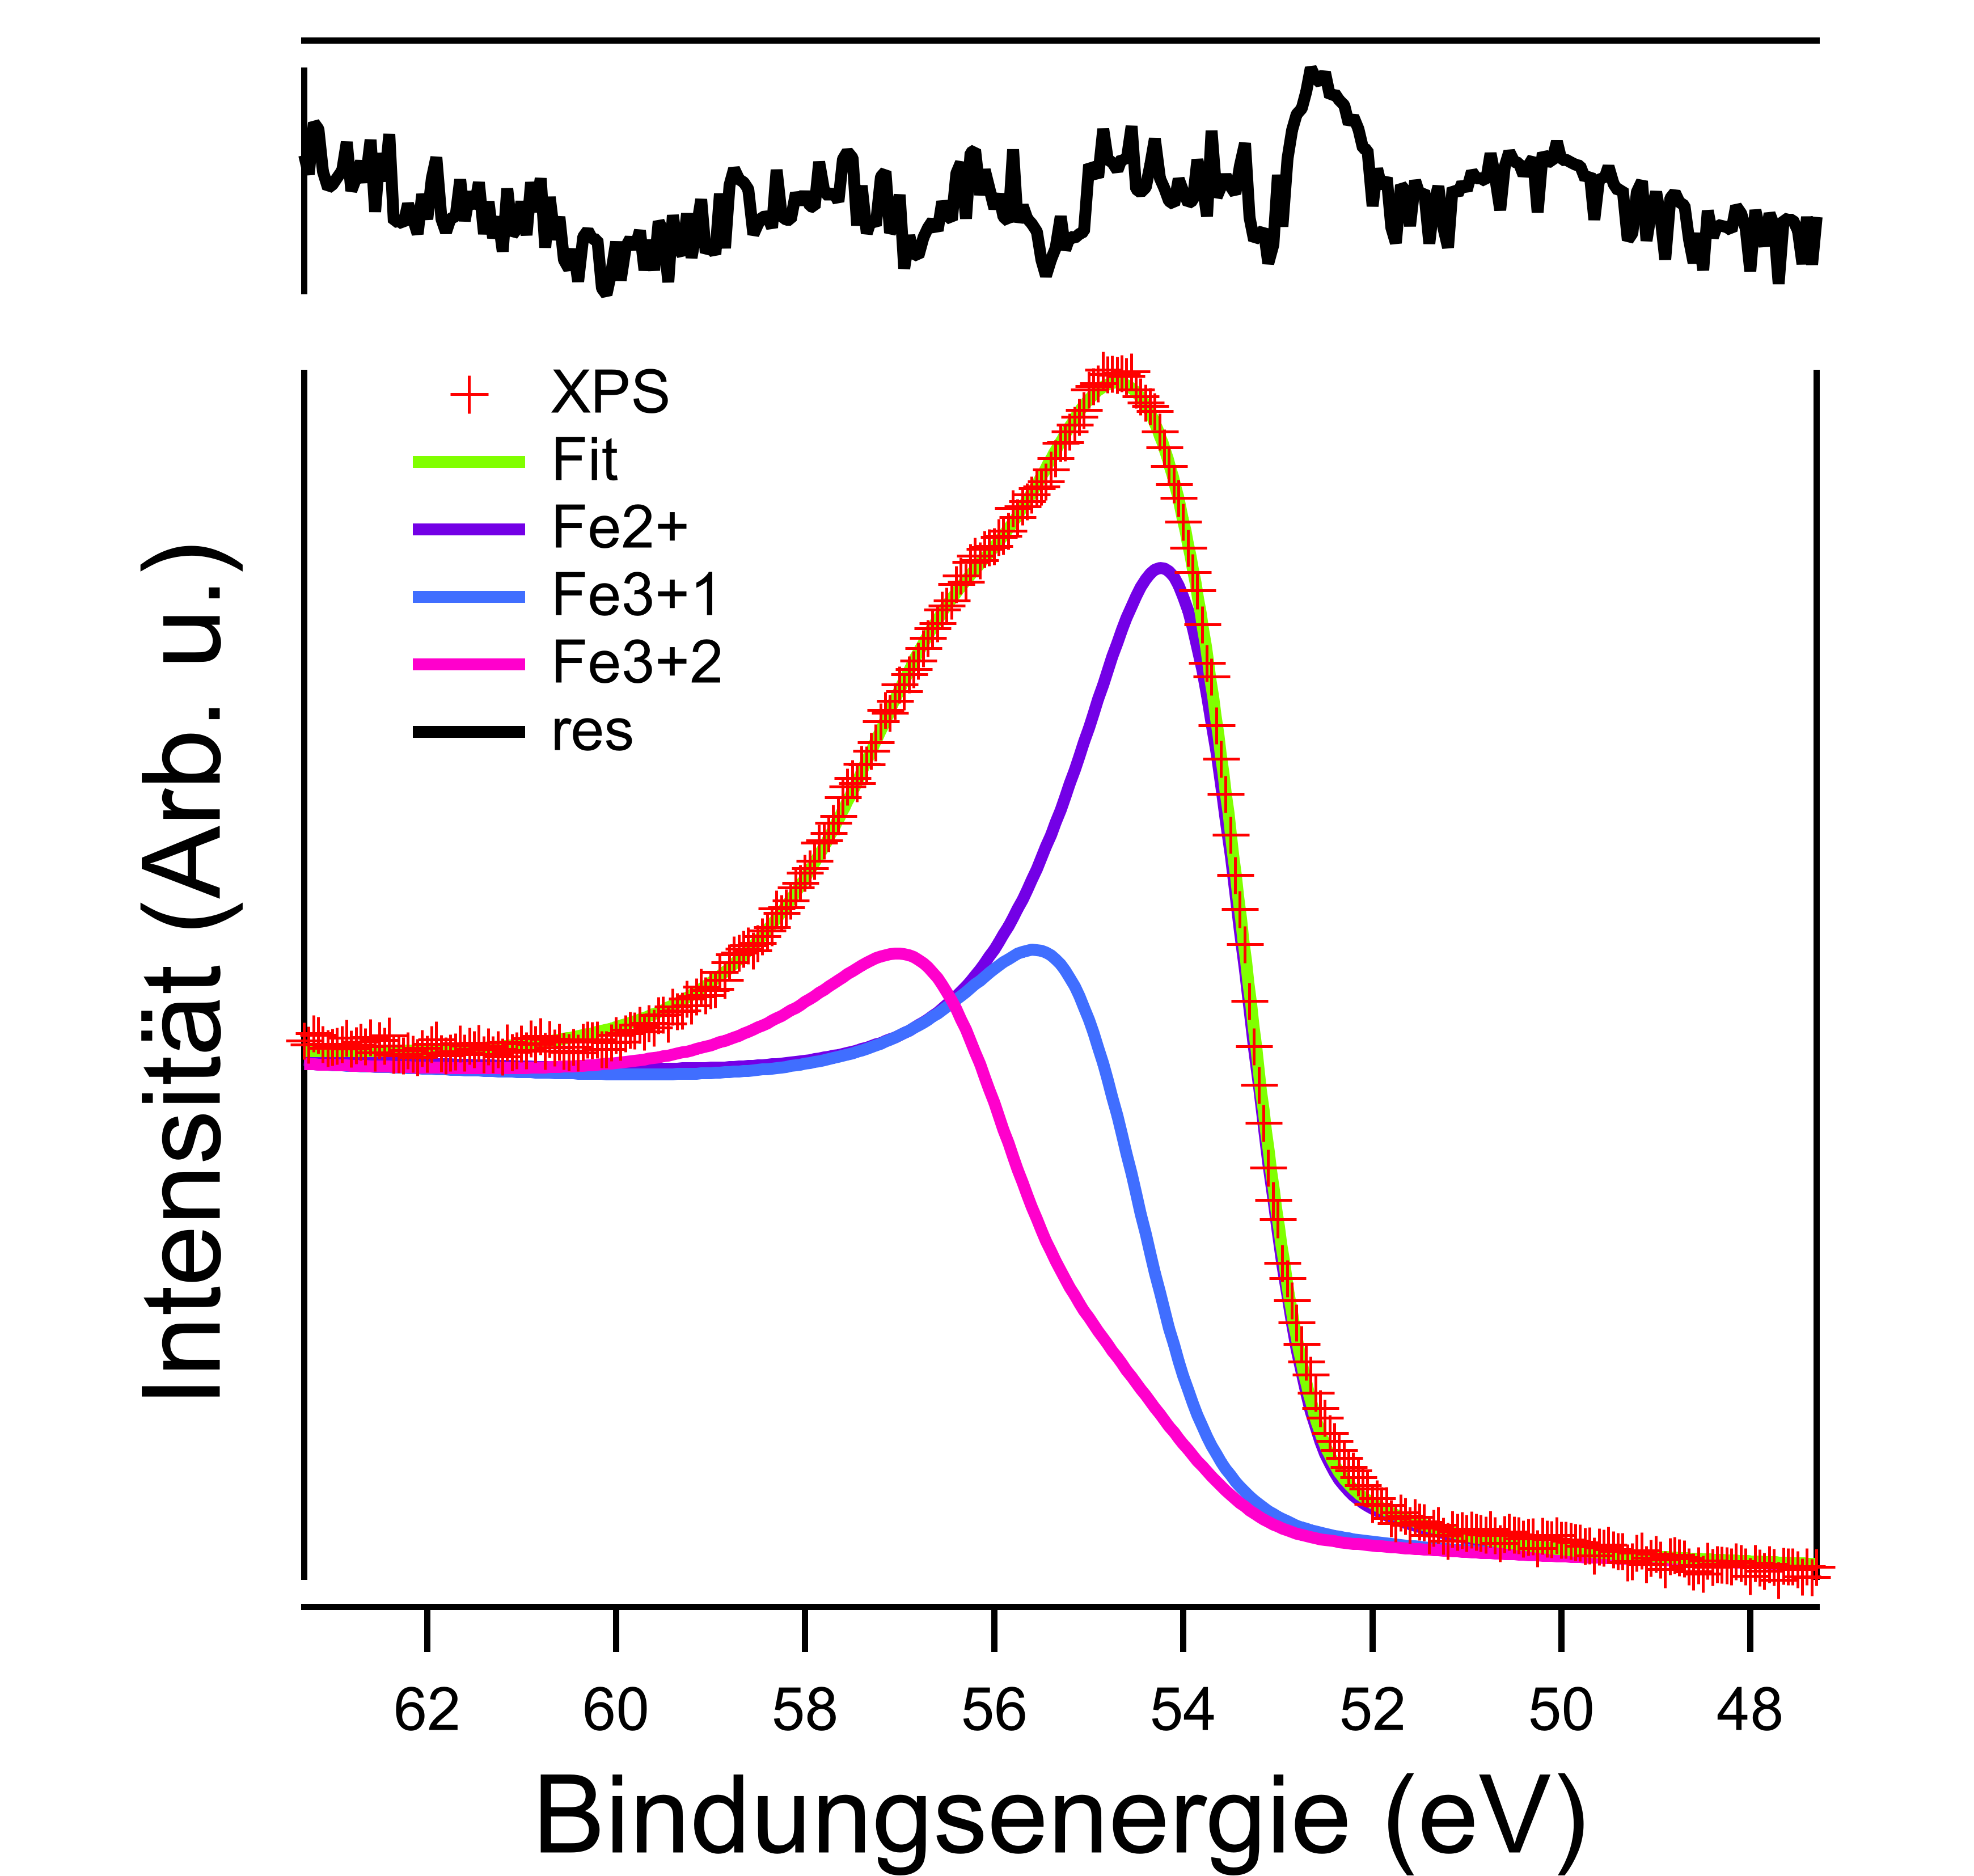
\includegraphics[height=6cm]{Fe3O4/Fe3p_Fe3O4_3.png}
                \subcaption{}
                \label{fig:XPSFe3p_Fe3O4}
            \end{subfigure}
            \begin{subfigure}[t]{0.48\textwidth}
                \centering
                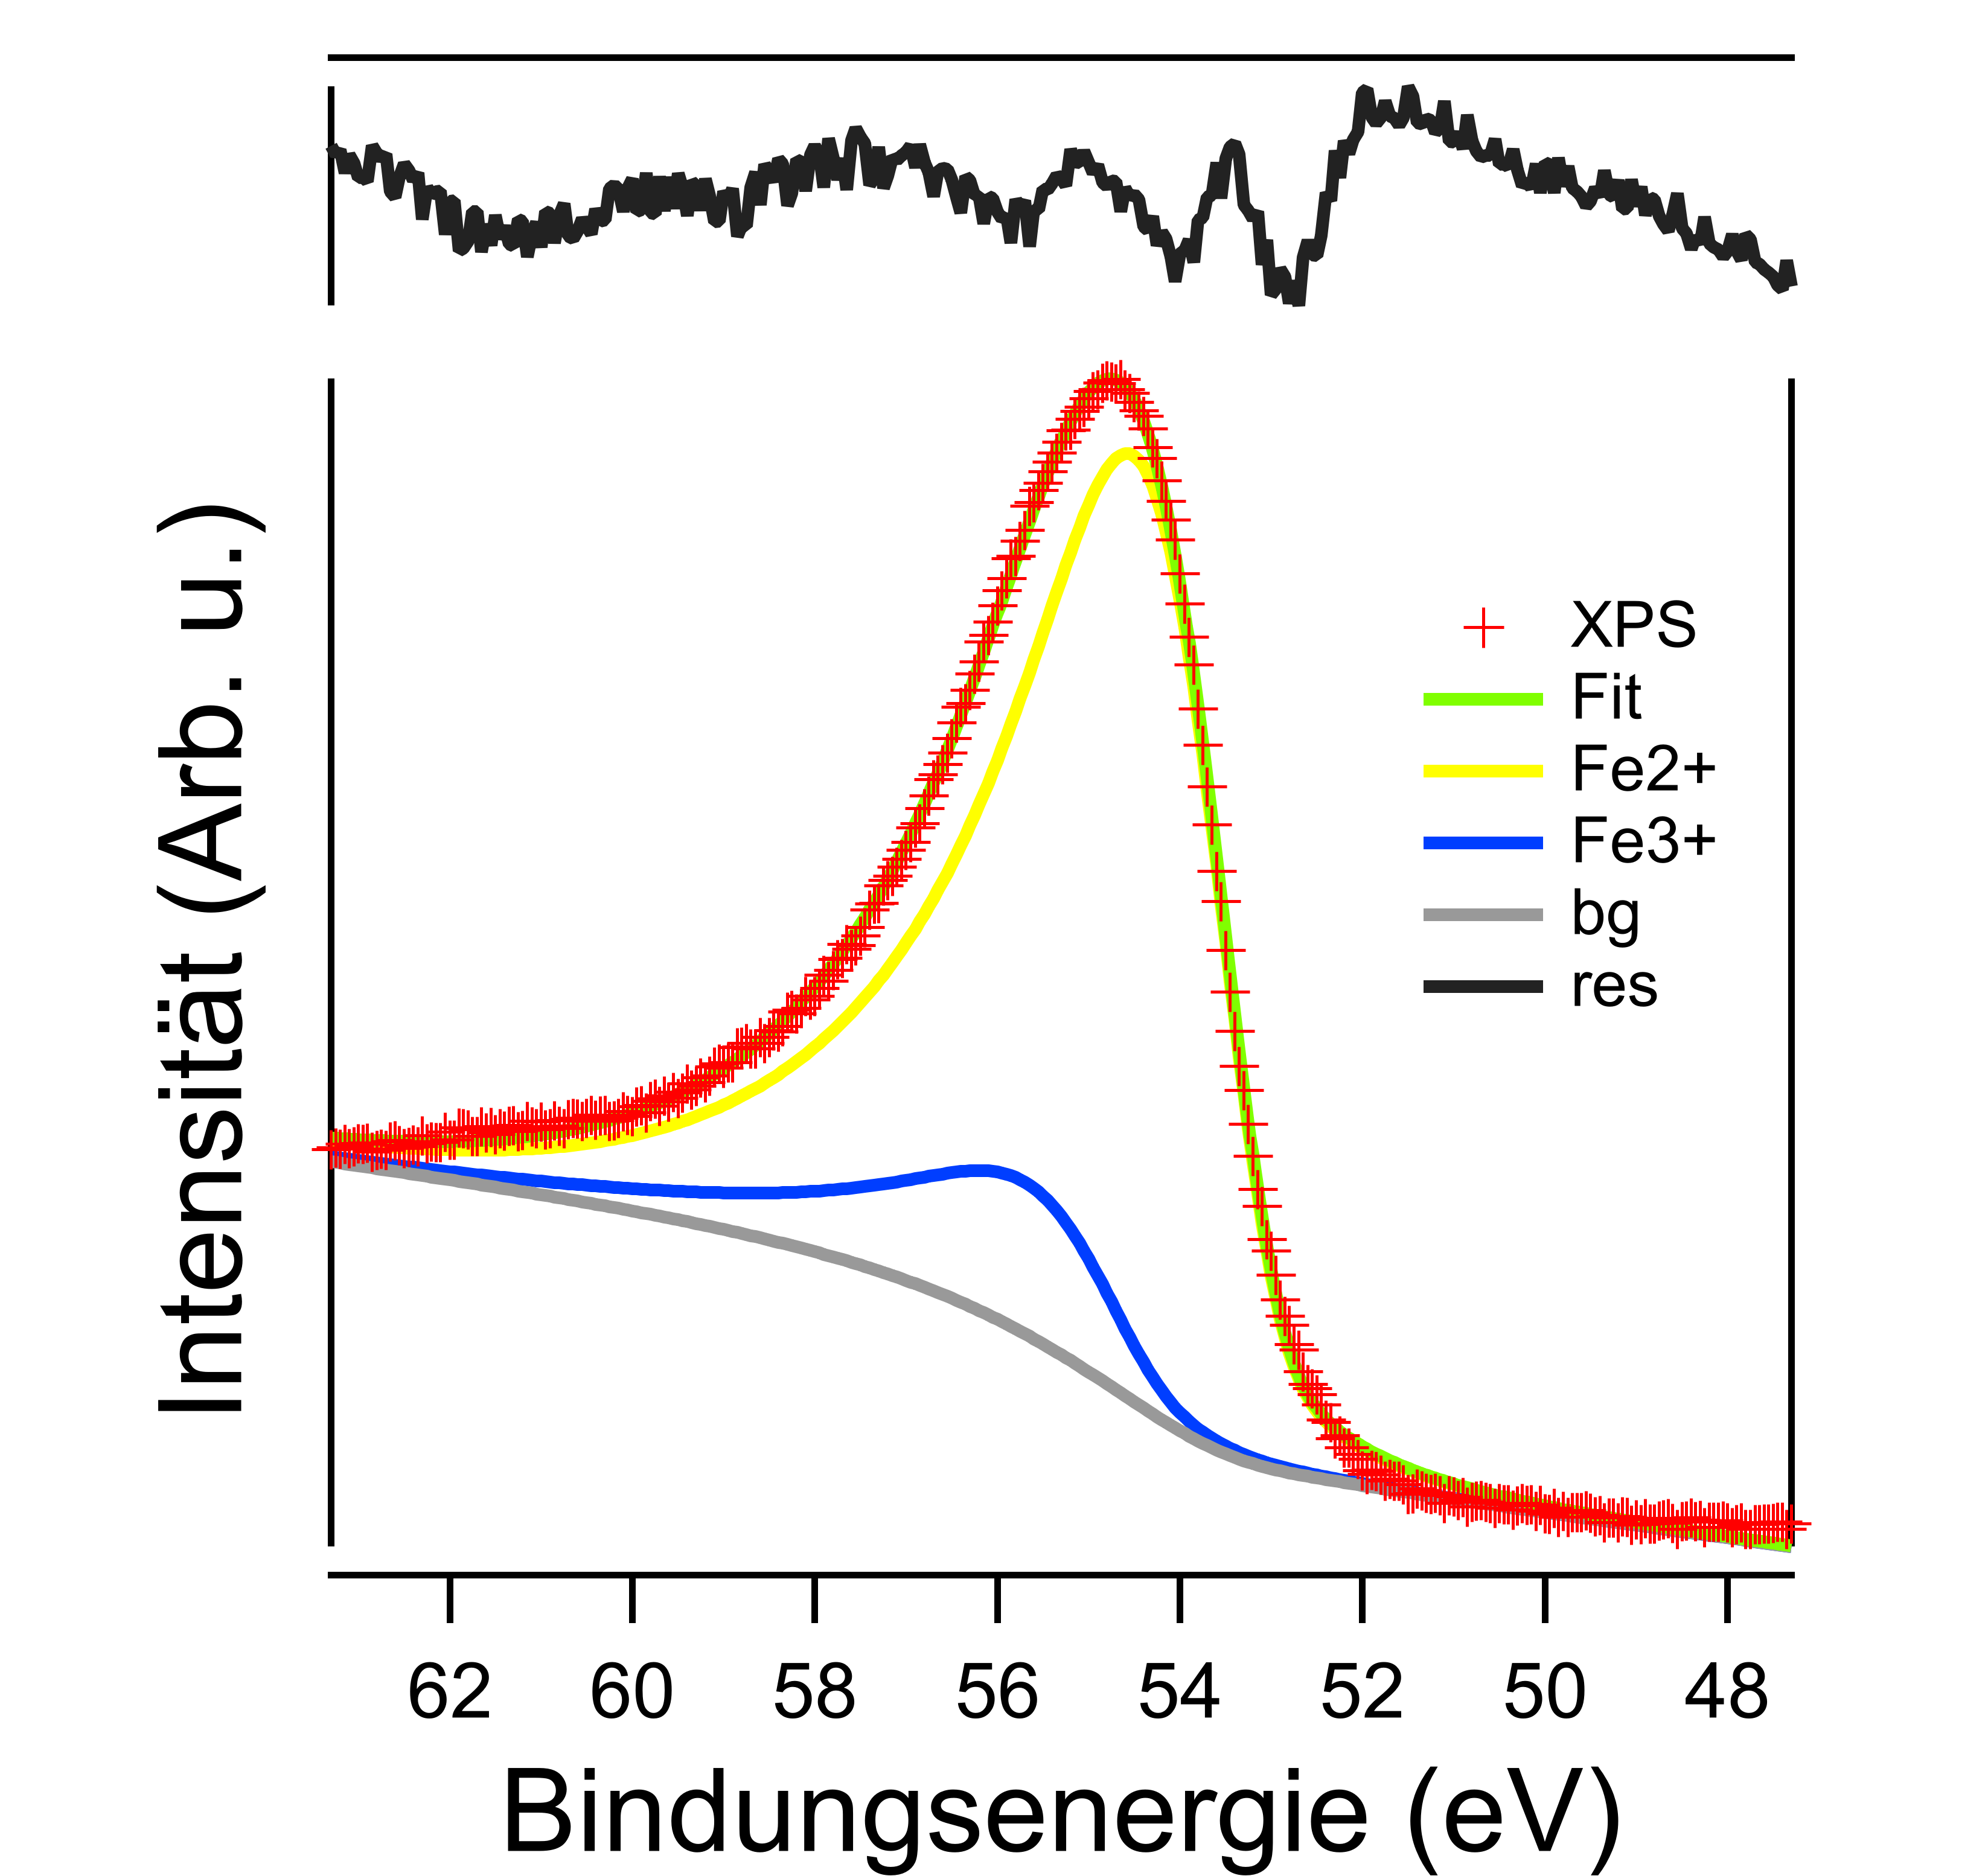
\includegraphics[height=6cm]{FeO/Fe3p_FeO_3.png}
                \subcaption{}
                \label{fig:XPSFe3p_FeO}
            \end{subfigure}
            \caption{Die Röntgenphotoelektronenspektroskopie Spektren bei einer Photonenenergie von \SI{200}{\electronvolt} der $\ce{Fe}_\text{3p}$-Zustände mit s-polarisierter Strahlung.
            In (\subref{fig:XPSFe3p_Fe3O4}) das Spektrum des aufgedampften Films, sowie des modifizierten Films in (\subref{fig:XPSFe3p_FeO}).}
            \label{fig:XPS_Fe3p}
        \end{figure}
        Im Gegensatz zu dem Kerniveau des Sauerstoffs zeigen sich in den XPS-Spektren des $\ce{Fe}_{3\text{p}}$-Kernniveau in \autoref{fig:XPS_Fe3p} deutliche Veränderungen.
        So zeigt das Spektrum nach dem ioneninduzierten Zerstäuben und Aufheizen keine ausgeprägte Schulter zu höheren Bindungsenergien.
        Diese Schulter wird maßgeblich durch den Anteil an $\ce{Fe}^{3+}$-Ionen hervorgerufen~\cite{FeO_7}.
        Ein höheres Sauerstoffangebot kann zu einem erhöhten Oxidationszustand führen.
        Unter der Annahme, dass es sich bei dem aufgedampften Film um Magnetit handelt werden drei beitragende Signale erwartet~\cite{FeO_55}.
        Diese rühren vom $\ce{Fe}^{2+}$ bei niedrigen Bindungsenergien und bei höheren vom $\ce{Fe}^{3+}$ her.
        Letzteres befindet sich zum Einen in einer oktaedrischen wie auch tetraedrischen Umgebung, was ebenfalls zu einer Energieverschiebung führt~\cite{FeO_12}.
        Um die Gesamtintensität zu beschreiben wurde ein Shirley-Untergrund gemeinsam mit drei Pseudo-Voigt-Funktionen mit einer Asymmetrie von \num{0.3} und einer Halbwertsbreite von \SI{2.7}{\electronvolt} angepasst.
        So ergaben sich die einzelnen Positionen zu \SI{54.1}{\electronvolt}, \SI{55.3}{\electronvolt} und \SI{56.8}{\electronvolt}.
        Hiermit wurde ein bessere Anpassung erzielt als bei der Verwendung von nur zwei Pseudo-Voigt-Funktionen, die einen $\ce{Fe}^{2+}$- und $\ce{Fe}^{3+}$-Anteil darstellen würden. 
        Der Beitrag des niederenergetischen Signals liegt bei etwa \SI{60}{\percent} und wird dem $\ce{Fe}^{2+}$ zugeordnet.
        Für den $\ce{Fe}^{3+}$-Beitrag ergeben sich noch \SI{40}{\percent}.
        Erwartet wird bei Magnetit ein Verhältnis von 1:2~\cite{FeO_12, FeO_7}.

        Bei dem behandelten Film zeigt sich eine Verschmälerung der Gesamtintensität, als Folge der abwesenden Schulter bei größeren Bindungsenergien.
        Eine gute Approximation mit nur zwei Pseudo-Voigt-Funktionen mit der Halbwertsbreite von \SI{3.7}{\electronvolt} und einer Asymmetrie von \num{0.4} zeigt gute Evaluation des Signals~\cite{FeO_11, FeO_7}.
        Dabei ergeben sich die beiden Positionen der Anteile zu \SI{54.5}{\electronvolt} und \SI{55.7}{\electronvolt}.
        Erneut lässt sich eine relative Position der Bindungsenergien zum unbehandelten Film sehen, dies ist ebenfalls durch den Wechsel des Gitters des Monochromators zu erklären und liegt im selben Größenbereich von wenigen Elektronenvolt Zehnteln.
        Es lässt sich klar die Intensitätsverschiebung zu niedrigeren Energien hin erkennen.
        Der relative Anteil des $\ce{Fe}^{2+}$-Anteils liegt bei \SI{86}{\percent} wohingegen der des $\ce{Fe}^{3+}$ auf \SI{14}{\percent} gesunken ist.
        Der Anteil an $\ce{Fe}^{2+}$-Ionen ist also folglich gestiegen.

        Ein Vergleich mit der Literatur zeigt, dass sich zwischen dem $\ce{Fe}^{2+}$-Signal und $\ce{Fe}^{3+}$-Signal eine Verschiebung von etwa \SI{1.8}{\electronvolt} einstellt~\cite{FeO_15, FeO_12}.
        Für den unbehandelten Film passt dies recht gut, wenn die gewichtete Position der beiden $\ce{Fe}^{3+}$-Beiträge \SI{55.9}{\electronvolt} verwendet wird.
        Für den behandelten Film ergibt sich eine Verschiebung von \SI{1.2}{\electronvolt}.
        Eine Deutung der genauen Positionen der einzelnen Beiträge gestaltet sich als schwierig.
        Die Werte des $\ce{Fe}^{2+}$-Signal reichen in der Literatur von \SI{53.7}{\electronvolt} \cite{FeO_7} bis zu \SI{54.9}{\electronvolt} \cite{FeO_12}.
        Die verschiedenen Positionen können ebenfalls durch die verschieben Kompositionen hervorgerufen werden \cite{FeO_12}.
        Eine weitere Fehlerquelle könnte die Wahl der Asymmetrie und Anzahl der verwendeten Voigt-Funktionen sein.
        Manche Quellen sagen aufgrund der Feinstruktur sechs Beiträge voraus~\cite{FeO_14, FeO_17, FeO_15}, andere zwei ($\ce{Fe}^{2+}$, $\ce{Fe}^{3+}$)~\cite{FeO_15, FeO_11, FeO_10, FeO_7} oder drei ($\ce{Fe}^{2+}$, $\ce{Fe}^{3+}_\text{tetra}$, $\ce{Fe}^{3+}_\text{okta}$)~\cite{FeO_12, FeO_55} oder auch vier um die Spin-Bahn-Aufspaltung mit etwa \SI{1}{\electronvolt} einzubeziehen~\cite{FeO_55}.
        Die Halbwertsbreite ist recht groß, da es bei High-Spin Zuständen zur Ausbildung von Multipletts kommt und diese nicht aufgelöst werden können~\cite{wandelt_photoemission_1982}.
        Die Asymmetrie kann durch Mehrfachionisation bei inneren Prozessen wie Augerzerfällen oder durch mehrere Photonen begründet werden~\cite{FeO_55}.

        \begin{figure}
            \centering
            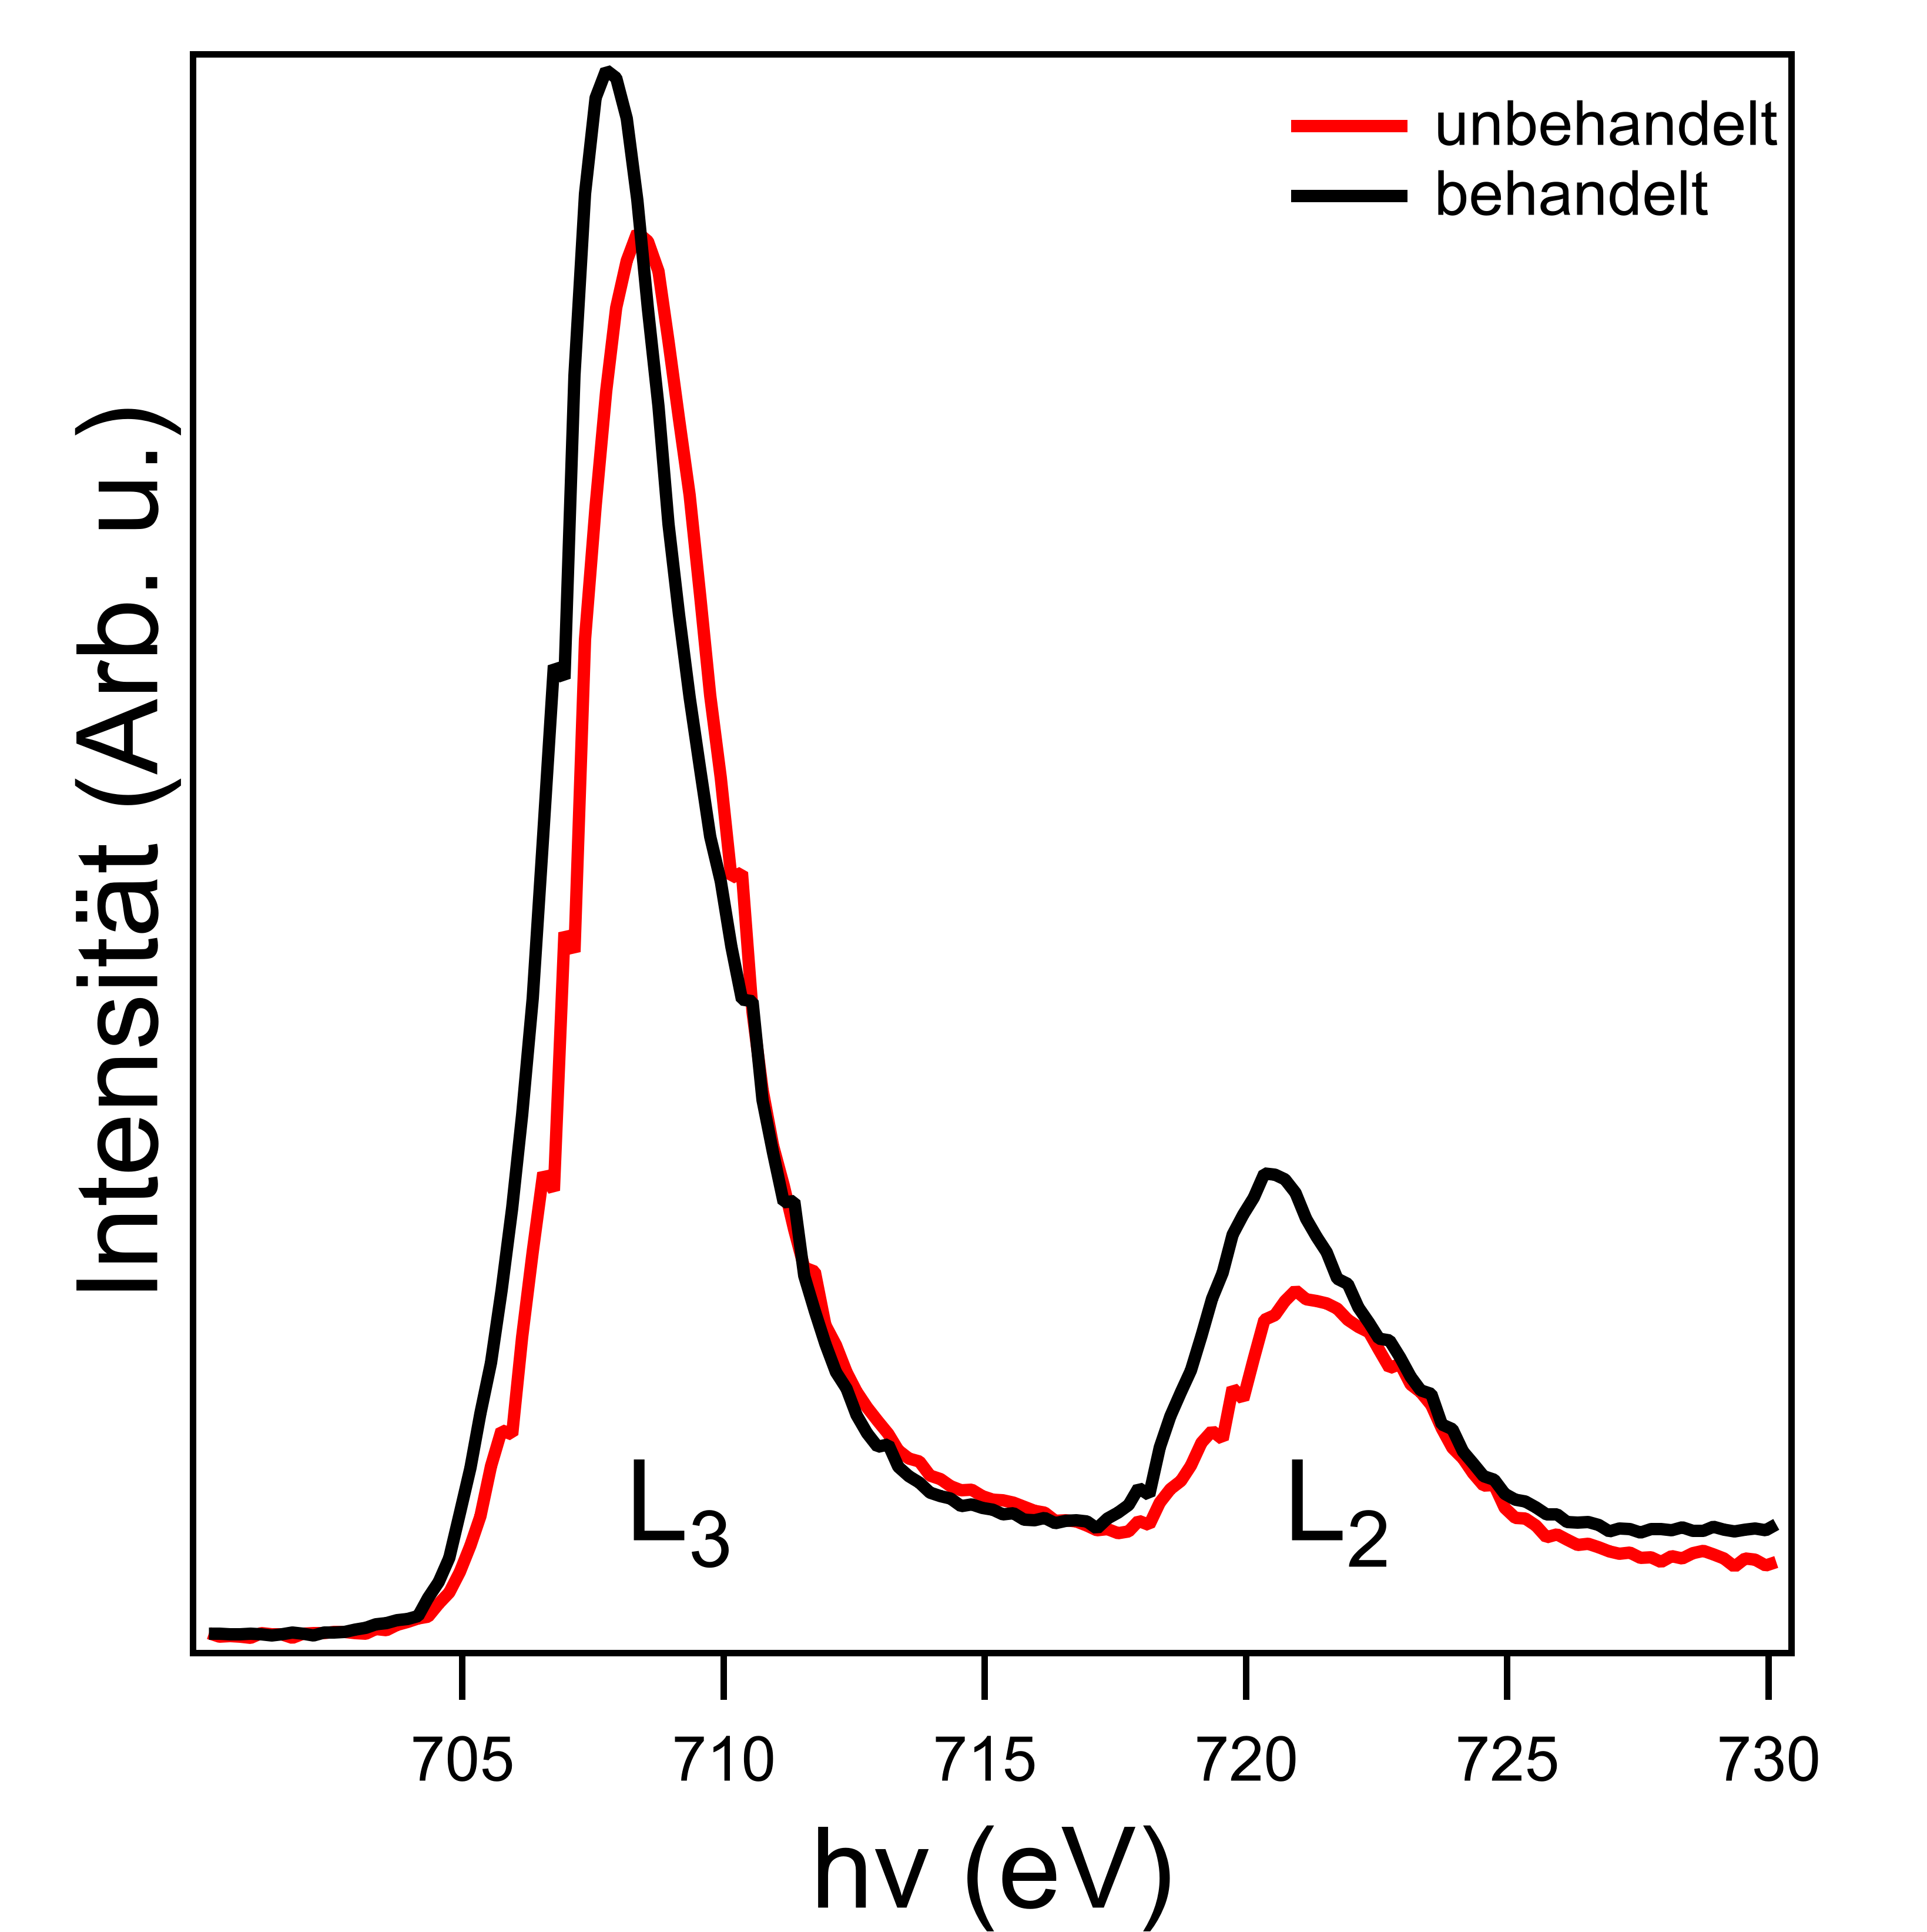
\includegraphics[height=6cm]{XAS_cp_corr.png}
            \caption{Die Röntgenabsorptionsspektren des aufgedampften Films (rot) und des bearbeiten Films (schwarz).
            Aufgenommen mit rechtszirkular polarisiertem Licht und Teilelektronenausbeute von Sekundärelektronen bei einer Energie von $E_\text{Kin} = \SI{7}{\electronvolt}$.}
            \label{fig:XAS}
        \end{figure}
        Beim Vergleich zwischen dem Röntgenabsorptionsspektrum des unbehandelten Films, sowie des behandelten Films in \autoref{fig:XAS} fällt auf, dass sich das Signal der $\text{L}_3$-Absorptionskante zu kleineren Photonenenergie hin verschoben hat.
        Die Verschiebung beträgt etwa \SI{0.4}{\electronvolt} und ist korreliert mit dem Oxidationszustand~\cite{chen_nexafs_1997}.
        Mit steigendem Oxidationszustand steigt ebenfalls die Absorptionsenergie des $\text{L}_3$-Übergangs~\cite{chen_nexafs_1997, FeO_71}.
        Hierbei wird aus der Literatur ein relative Verschiebung zum Eisensignal von \SI{0.3}{\electronvolt} für $\ce{Fe}^{2+}$-Ionen und \SI{0.7}{\electronvolt} für $\ce{Fe}^{3+}$-Ionen erwartet~\cite{FeO_71}.
        Röntgenabsorptionsmessungen wurden am reinen Eisen nicht vorgenommen, allerdings ist der relative Versatz der beiden Filme passend zur Konzentration der erwarteten Ionensorten.
        Durch die Behandlung steigt folglich der $\ce{Fe}^{2+}$-Anteil und gleichfalls sinkt der $\ce{Fe}^{3+}$-Anteil.
        Dies wird durch den erhöhten Beitrag bei \SI{707}{\electronvolt} begründet, welcher für \ce{FeO} mit einer leichten Schulter zu \SI{709}{\electronvolt} beobachtet wurde~\cite{FeO_45}.
        Für Magnetit verhält sich dies genau umgekehrt~\cite{FeO_45}.
        Auch die Breite der $\text{L}_3$-Absorptionskante steigt vom unbehandeltem zum behandelten Film an.
        Dies ist für eine kleinere Beteiligung von größeren Oxidationszuständen zu erwarten~\cite{chen_nexafs_1997}.
        % Erklärung findet dies, da die Röntgenabsorptionsspektroskopie die leeren Valenzbandzustände untersucht.
        Leere Valenzbandzustände der Oxide sind lokalisierter als die des Metalls, was zu einer Verlängerung der Lebenszeit und damit verknüpften kleineren Halbwertsbreite kommt~\cite{XMCD_XMLD}.
        Klar erkennbar ist ebenfalls die verbreiterte Struktur der $\text{L}_2$-Absorptionskante zwischen dem behandeltem und unbehandeltem Film.
        Bei dem unbehandelten Film ist die aus der Literatur bekannte Doppelspitze nicht sehr ausgeprägt, wohingegen sich bei dem behandelten Film nur eine Spitze wie erwartet ausbildet~\cite{FeO_45}.
        Die allgemeine Struktur dieser Spektren ist recht schwierig zu beschreiben und unterscheidet sich deutlich bei unterschiedlichen Oxiden~\cite{FeO_46}, was sich hier allerdings nicht erkennen lässt.
        % Kristallfeld und Multiplett-Effekte bestimmen die Zustände im Valenzbandbereich~\cite{XMCD_XMLD}.        

        Im Zusammenspiel der zur Charakterisierung genutzten Methoden lässt sich sagen, dass es sich bei dem direkt aufgedampften Film um keine sauber präparierte Magnetit Oberfläche handelt.
        Hierzu sind die Abweichungen in der erwarteten LEED-Struktur für die gewünschte Orientierung zu groß.
        Ebenso die Abweichung bei den Augerspektrum zum erwarteten Wert der Intensität Verhältnisse.
        Auch wenn das Valenzband eine einigermaßen gute Übereinstimmung zeigt so deuten doch die restlichen Methoden nicht auf reines Magnetit hin.
        Recht große Abweichungen gibt es bei der Anpassung des $\ce{Fe}_\text{3p}$-Signals im XPS Spektrum.
        Bei der Röntgenabsorptionsmessungen zeigt sich ein leichte Abweichung zu der aus der Literatur erwarteten Struktur.
        Vielmehr scheint es sich also um eine gemischte Phase als um reines Magnetit zu handeln.
        Da es sich nur um eine Zwischenphase zur Präparation des Eisenmonoxid handelt wird auf eine weiter Charakterisierung und das Aufbringen von Molekülen verzichtet.

        Beim behandelten FIlm zeigen sich nur leichte Abweichungen zu den Erwartungen bei den unterschiedlichen Messmethoden.
        Auf Grund der metastabilen Phase bei Raumtemperatur und nicht-stöchiometrischen Verbindung lassen sich diese aber tolerieren und es kann davon ausgegangen werden, dass es sich um Wüstit handelt.

        \begin{figure}
            \begin{subfigure}[t]{0.34\textwidth}
                \centering
                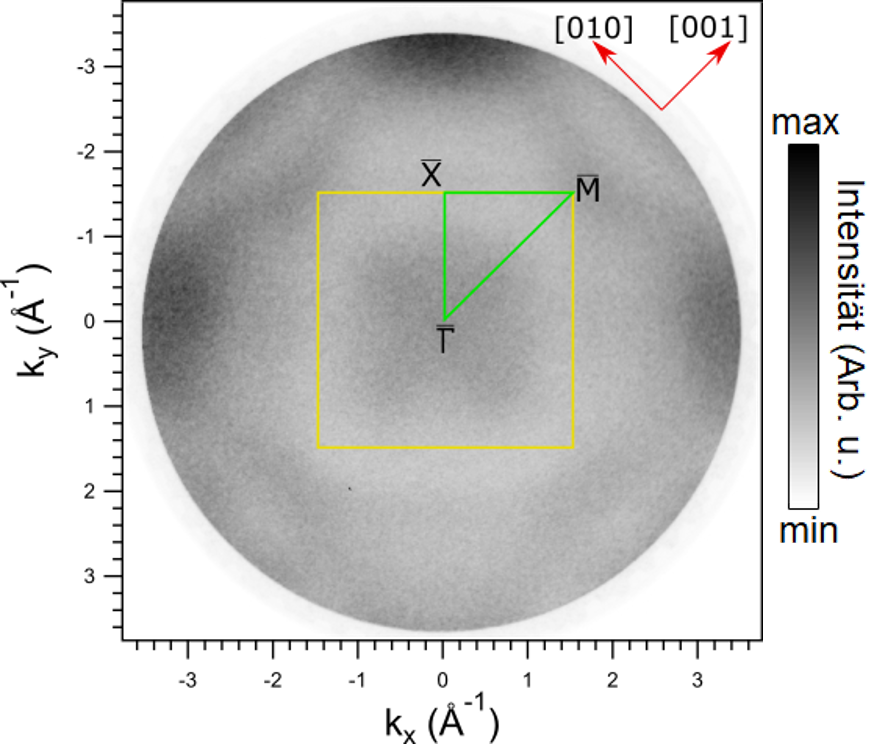
\includegraphics[height=4cm]{FeO/BZ_FeO.png}
                \subcaption{}
                % Die Brillouinzone des Eisensoxid bei einer Bindungsenergie von \SI{1.95}{\electronvolt}.
                % Eigezeichnet sind auch die Vektoren, sowie einige Hochsymmetrierichtungen.
                % Die Kantenlänge der BZ ist $\frac{2\pi}{a}\sqrt{2} = \SI[per-mode=reciprocal]{2.89}{\per\angstrom}$.
                % Im Zentrum liegt der $\overline{\Gamma}$-Punkt, der Abstand zum $\overline{X}$-Punkt ist $\frac{2\pi}{2 \cdot a}\sqrt{2} = \SI[per-mode=reciprocal]{1.45}{\per\angstrom}$ und zum $\overline{M}$-Punkt $\frac{2\pi}{a} = \SI[per-mode=reciprocal]{2.05}{\per\angstrom}$~\cite{Hüfner}.
                % Verwendete Photonenenergie war \SI{64}{\electronvolt} und die Polarisation p.}
                \label{fig:BZ_FeO}
            \end{subfigure}
            \begin{subfigure}[t]{0.62\textwidth}
                \centering
                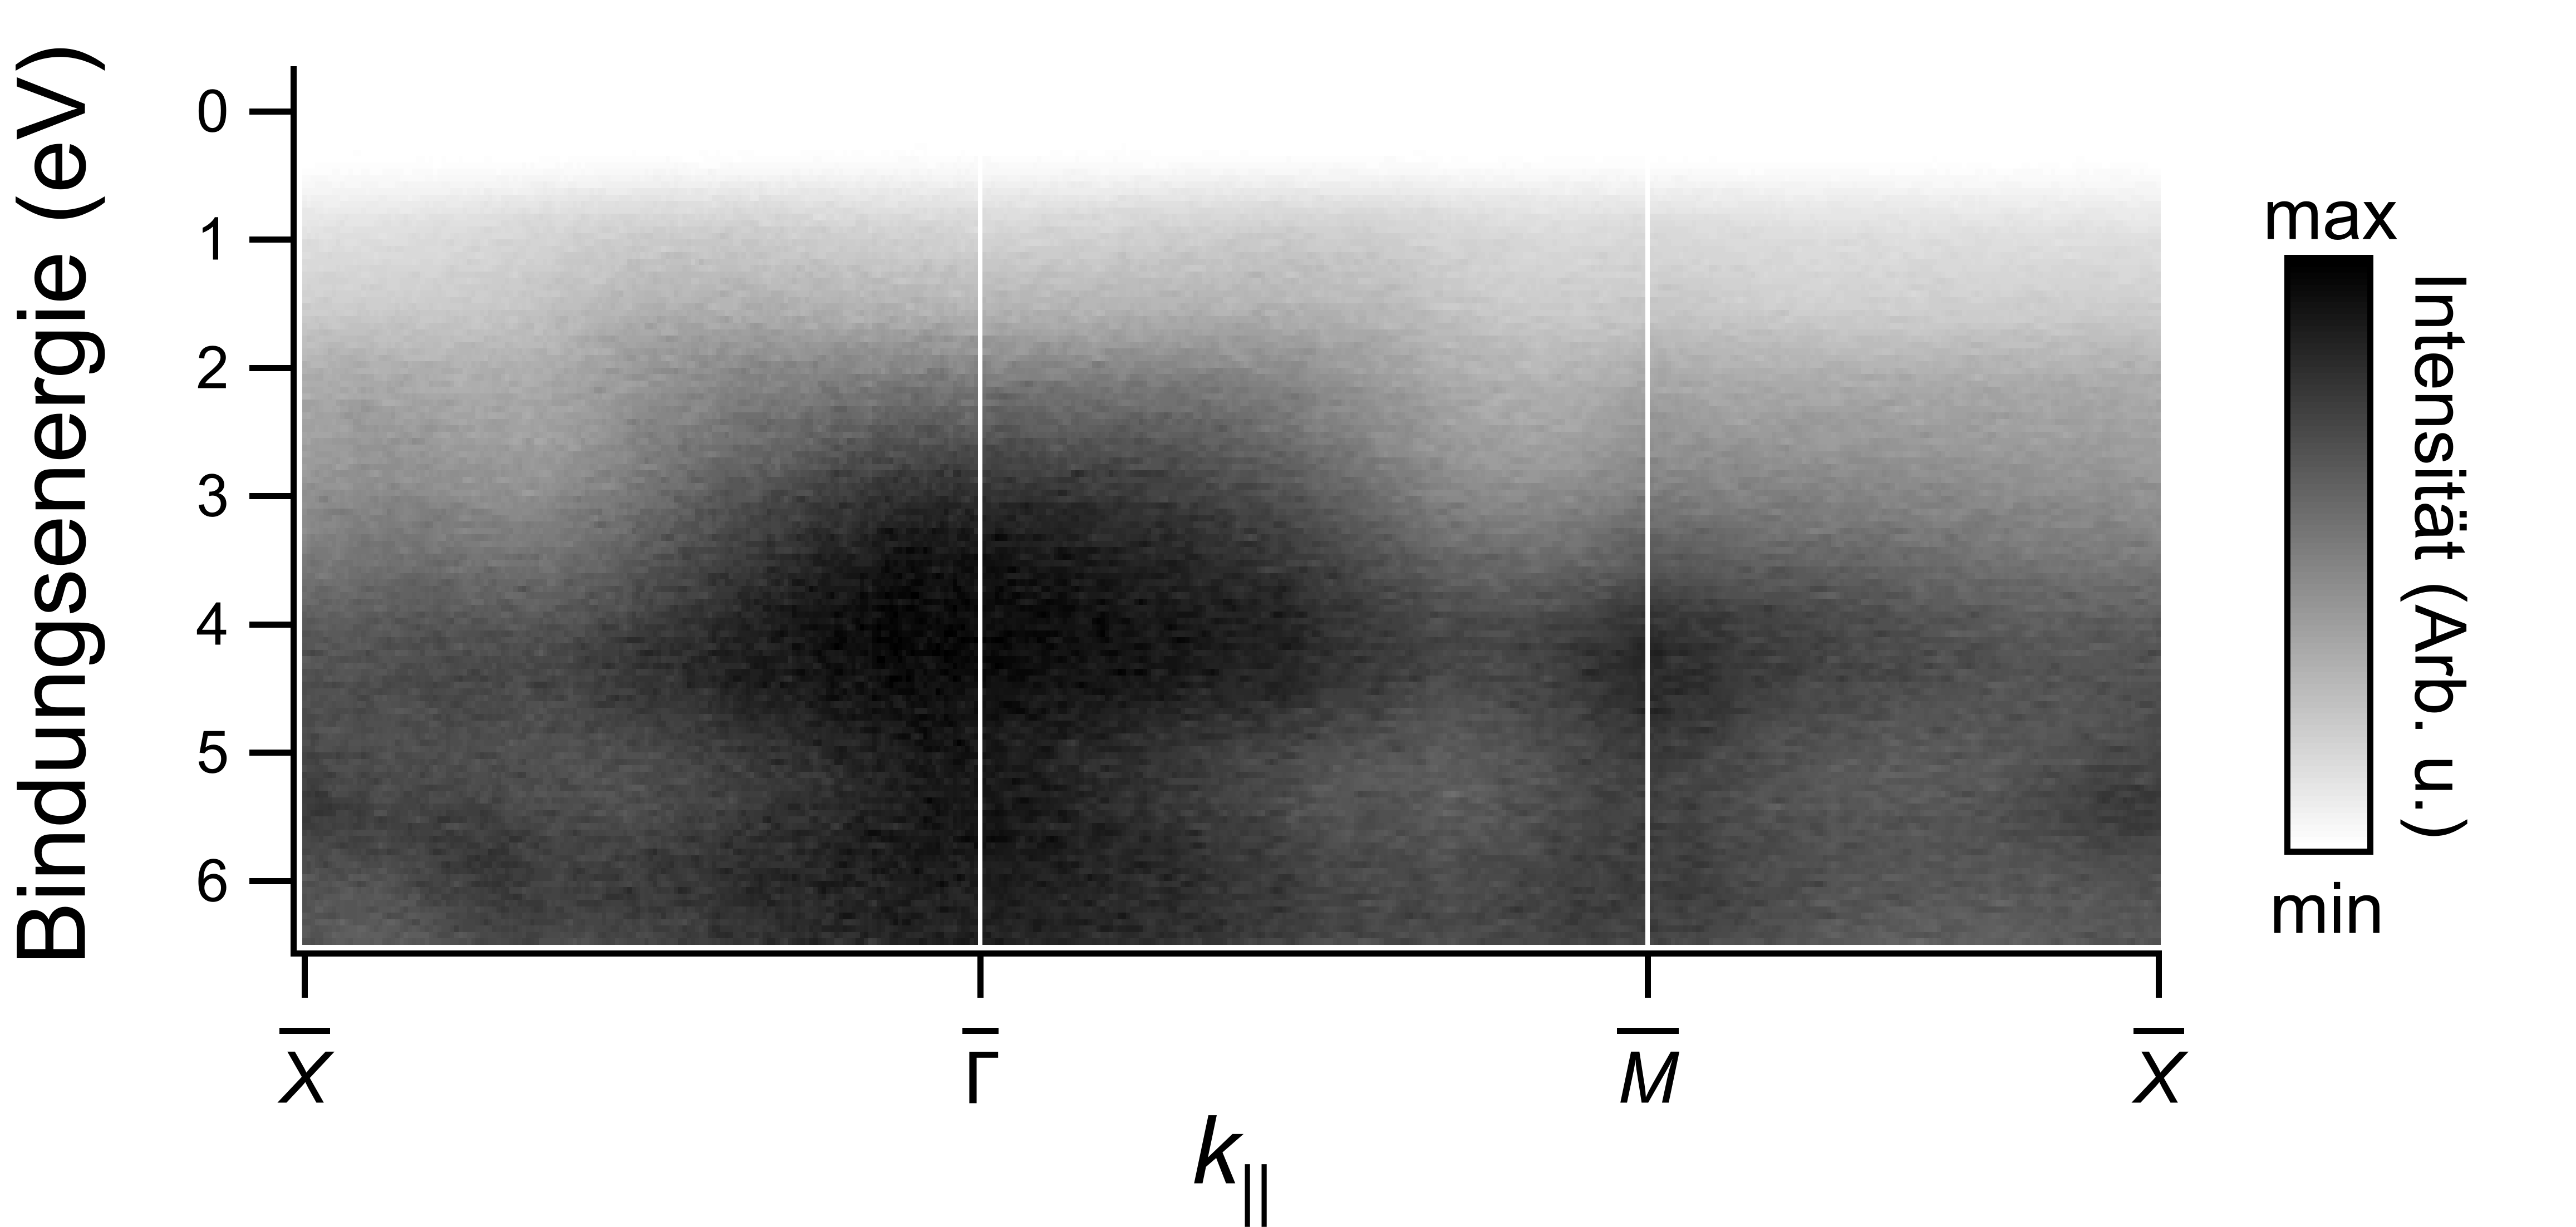
\includegraphics[height=4cm]{FeO/Band_FeO_2.png}
                \subcaption{}
                % Die Bandstruktur des Eisenmonooxid entlang einiger Hochsymmetrierichtungen.
                % Verwendete Photonenenergie war \SI{64}{\electronvolt} und die Polarisation p.
                \label{fig:Band_FeO}
            \end{subfigure}
            \caption{Die Oberflächenbrillouinzone des Eisenmonooxid bei einer Bindungsenergie von \SI{1.95}{\electronvolt} (\subref{fig:BZ_FeO}).
            Die entlang der grünen Linien aus (\subref{fig:BZ_FeO}) extrahierte Bandstruktur bei $h\nu = \SI{64}{\electronvolt}$ (\subref{fig:Band_FeO}).}
        \end{figure}
        Für die wohldefinierte Phase des Wüstits lässt sich auch die Oberflächenbrillouinzone definieren, die in \autoref{fig:BZ_FeO} abgebildet ist.
        Daraus lässt sich durch Schneiden des dreidimensionalen Datensatzes die Bandstruktur gewinnen, welche in \autoref{fig:Band_FeO} zu sehen ist.
        Wie schon beim Eisen reicht die Auflösung nicht aus um die Bänder klar zu separieren.
        Auffällig ist allerdings, dass sich die Intensität bezüglich des Eisens (vergleiche \autoref{fig:Band_Fe}) hin zu größeren Bindungsenergien verschoben hat.
        Dies lässt sich auf den Sauerstoffanteil in der Probe zurückführen. 
        Bei Eisen hingegen ergibt sich kein Beitrag durch Sauerstoff, sondern maßgeblich durch das d-Niveau nahe der Fermikante.
    
    \section{Pentacen auf Nickeloxid und Eisenmonooxid} \label{sec:Ergeb}
        Für die genauere Betrachtung von den Pentacen Molekühlen auf den antiferromagnetischen Substraten Nickeloxid (111) und Eisenmonooxid (100) muss zunächst die Molekülbedeckung evaluiert werden.
        Hierzu wird das Goldsubstrat (111) verwendet, da sich die Moleküle auf ihr in einer wohldefinierten Struktur anordnen~\cite{5A_4}.
        \begin{figure}
            \centering
            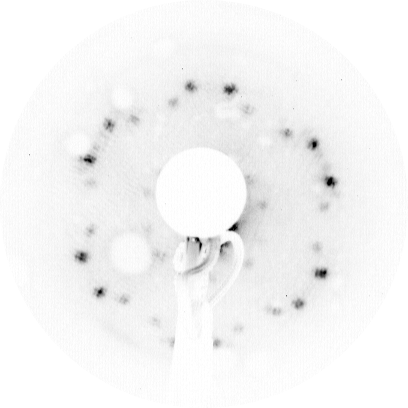
\includegraphics[height=5cm]{Au+5A/021_Au(111)+5A(40)_16eV.png}
            \caption{Evaluation der Monolagen Bedeckung des Pentacen auf der Oberfläche des Goldsubstrates bei einer Energie von \SI{16}{\electronvolt}.}
            \label{fig:LEED_Au+5A}
        \end{figure}
        Das entsprechende Beugungsbild ist in \autoref{fig:LEED_Au+5A} zu erkennen.
    
        \subsection{Pentacen auf Nickeloxid}
            \begin{figure}
                \centering
                \begin{subfigure}[t]{0.48\textwidth}
                    \centering
                    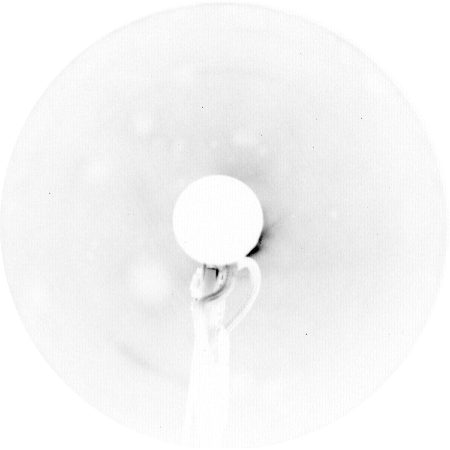
\includegraphics[height=5cm]{NiO+5A/2021_06_18_005_NiO111_5A_16eV.png}
                    \subcaption{}
                    \label{fig:LEED_NiO+5A_16}
                \end{subfigure}
                \begin{subfigure}[t]{0.48\textwidth}
                    \centering
                    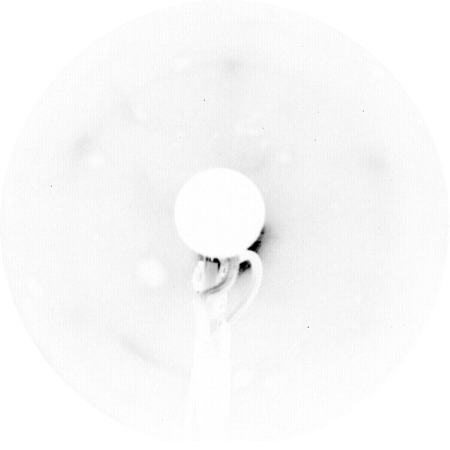
\includegraphics[height=5cm]{NiO+5A/2021_06_18_003_NiO111_5A_73eV.png}
                    \subcaption{}
                    % Die Bandstruktur des reinen Eisens entlang einiger Hochsymmetrierichtungen.
                    % Verwendete Photonenenergie war \SI{64}{\electronvolt} und die Polarisation p.
                    \label{fig:LEED_NiO+5A_73}
                \end{subfigure}
                \caption{Beugungsbild der niederenergetischen Elektronen für eine Monolage Pentacen auf der Nickeloxid (111) Oberfläche bei einer Elektronenenergie von \SI{16}{\electronvolt} (\subref{fig:LEED_NiO+5A_16}) und \SI{73}{\electronvolt} (\subref{fig:LEED_NiO+5A_73}).}
                \label{fig:LEED_NiO+5A}
            \end{figure}
            Das Aufdampfen von einer Monolage Pentacen bei dem Nickeloxid brachte kein LEED-Bild bei niedrigen Energien zustande (s. \autoref{fig:LEED_NiO+5A_16}), wie es für eine größere Überstruktur (z.B. bei Pentacen auf Gold in \autoref{fig:LEED_Au+5A}) erwartet wird.
            Bei größeren Energien in \autoref{fig:LEED_NiO+5A_73} hingegen sind leichte Substrateffekte des Nickeloxids sichtbar.
            So lässt sich schlussfolgern, dass sich die Moleküle auf der vorhandenen Oberfläche nicht in einer regelmäßigen Struktur anordnen.
            Dies gilt gleichermaßen für das Nickeloxid bei verschiedenen Schichtdicken.

            \begin{figure}
                \centering
                \begin{subfigure}[t]{0.30\textwidth}
                    \centering
                    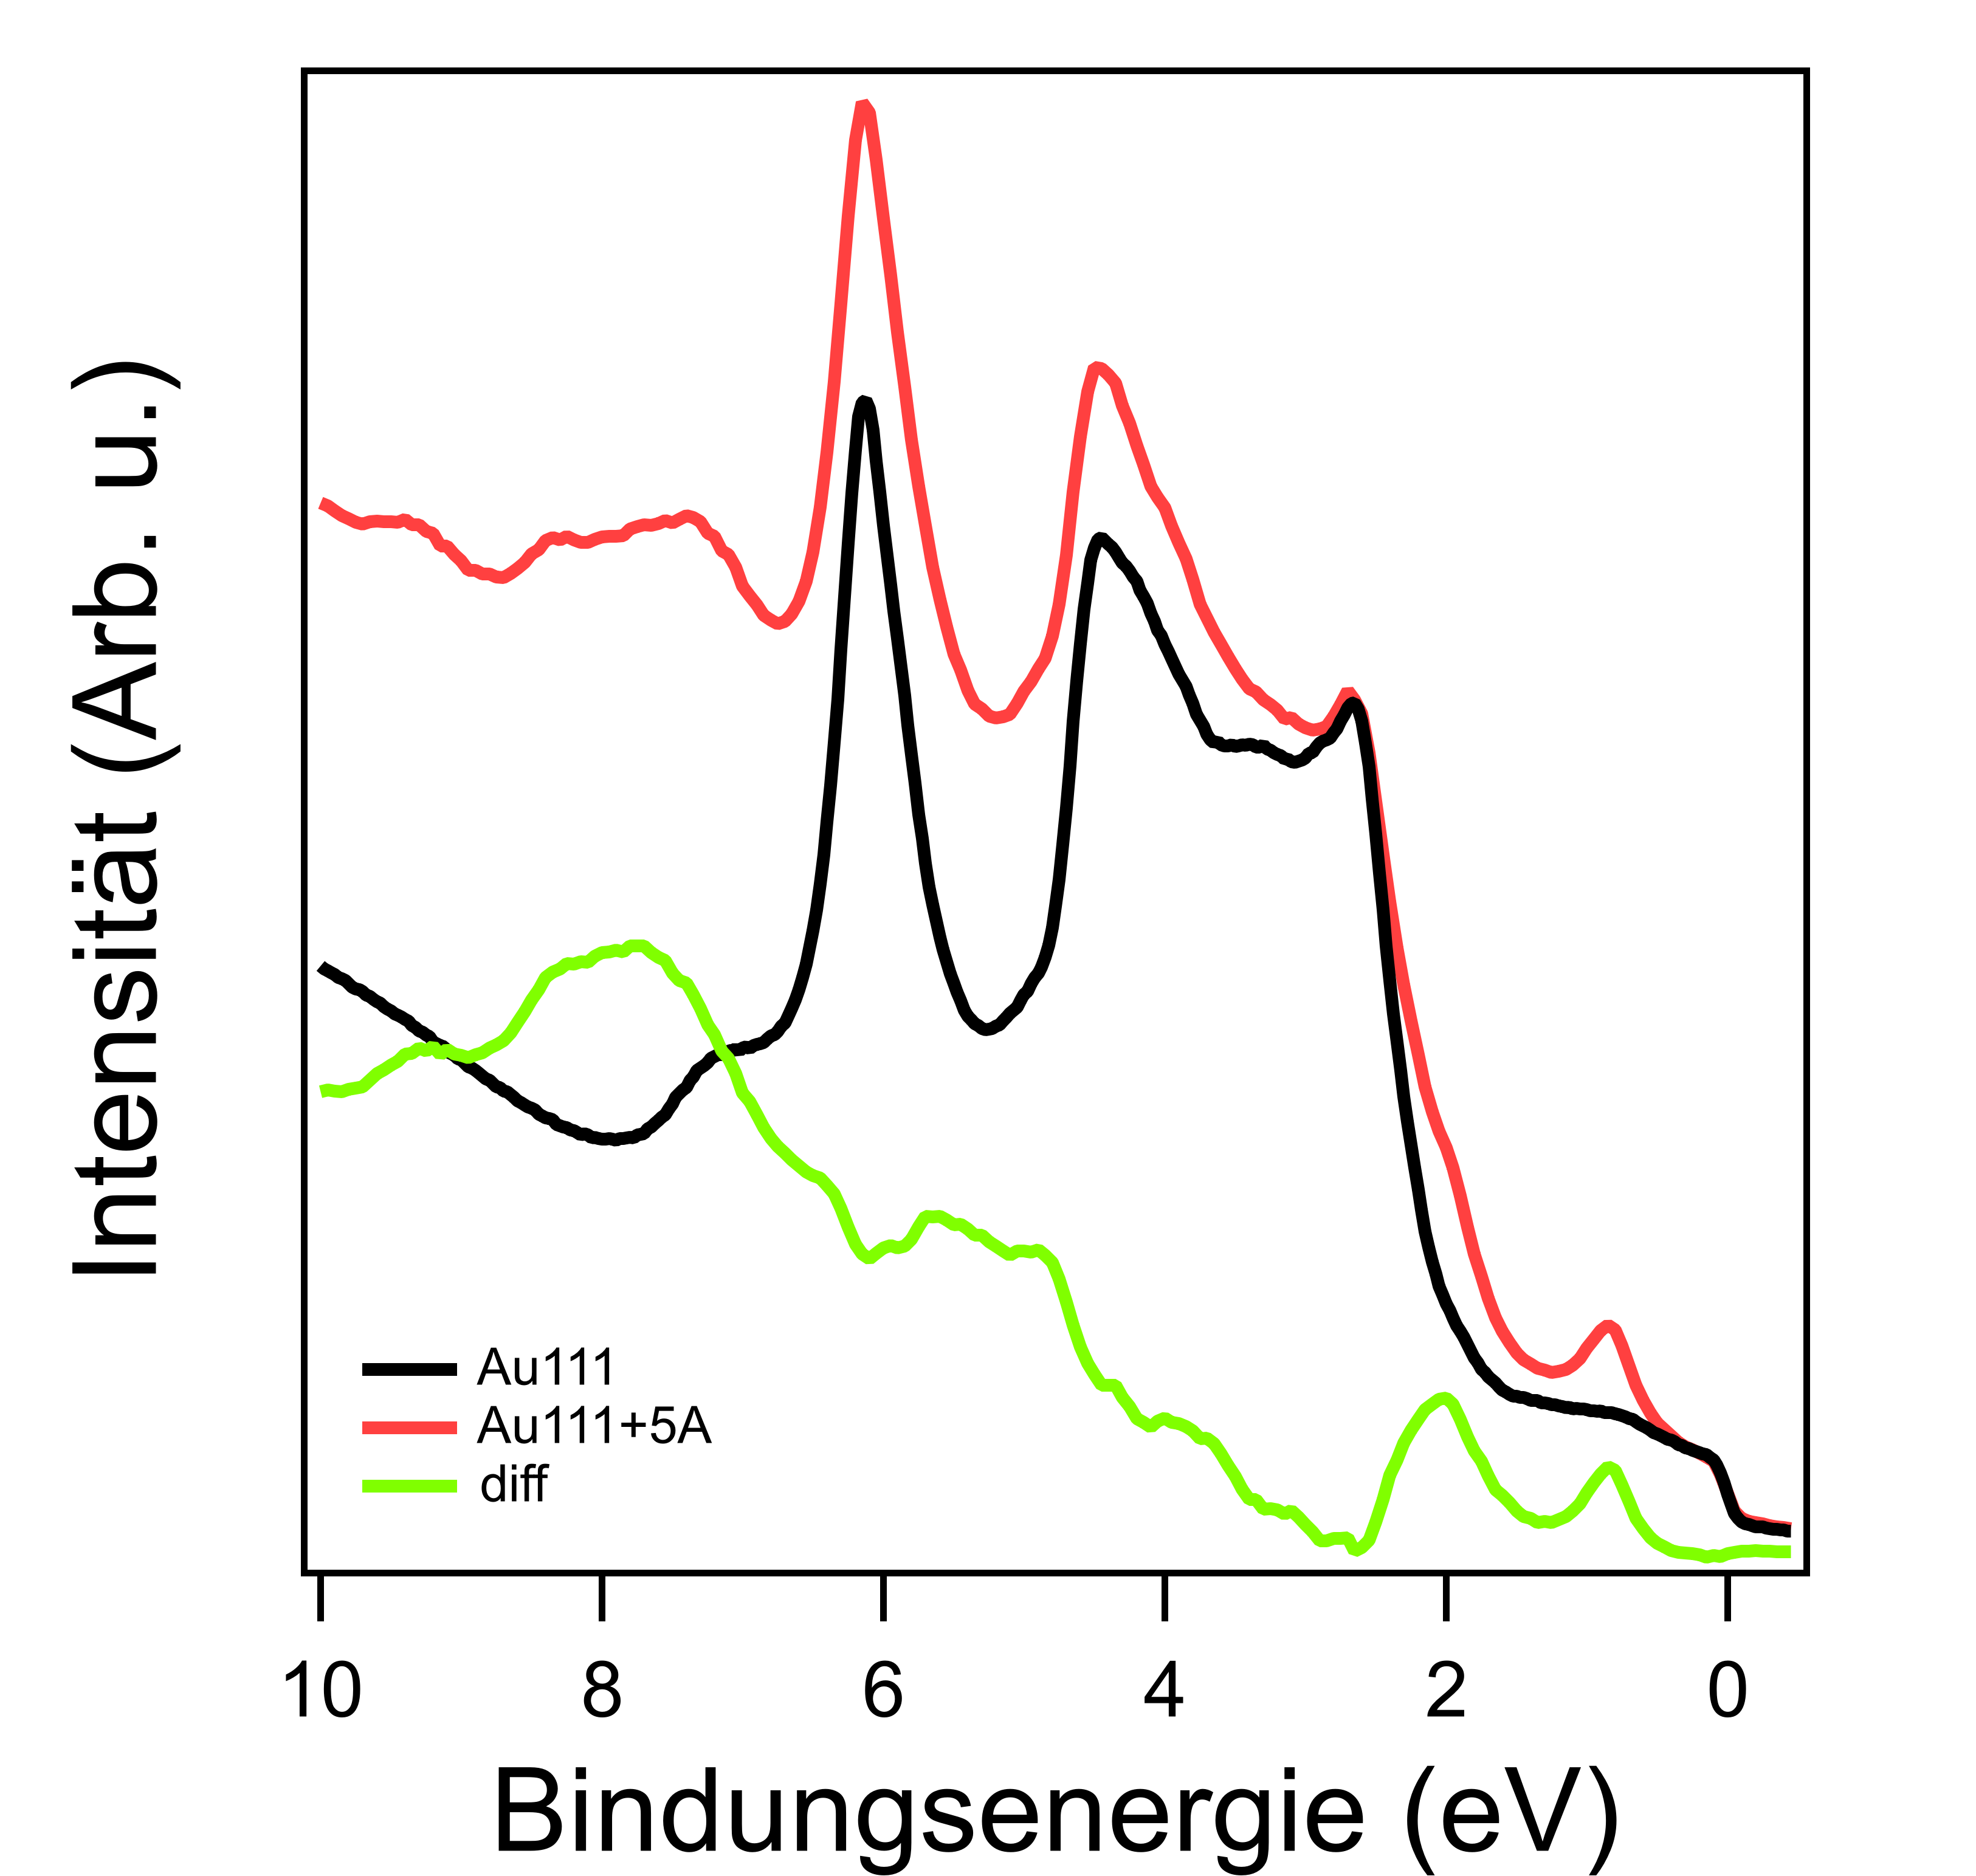
\includegraphics[height=4cm]{Au+5A/EDC_Au_5A.png}
                    \subcaption{}
                    \label{fig:EDC_Au+5A}
                \end{subfigure}
                \begin{subfigure}[t]{0.30\textwidth}
                    \centering
                    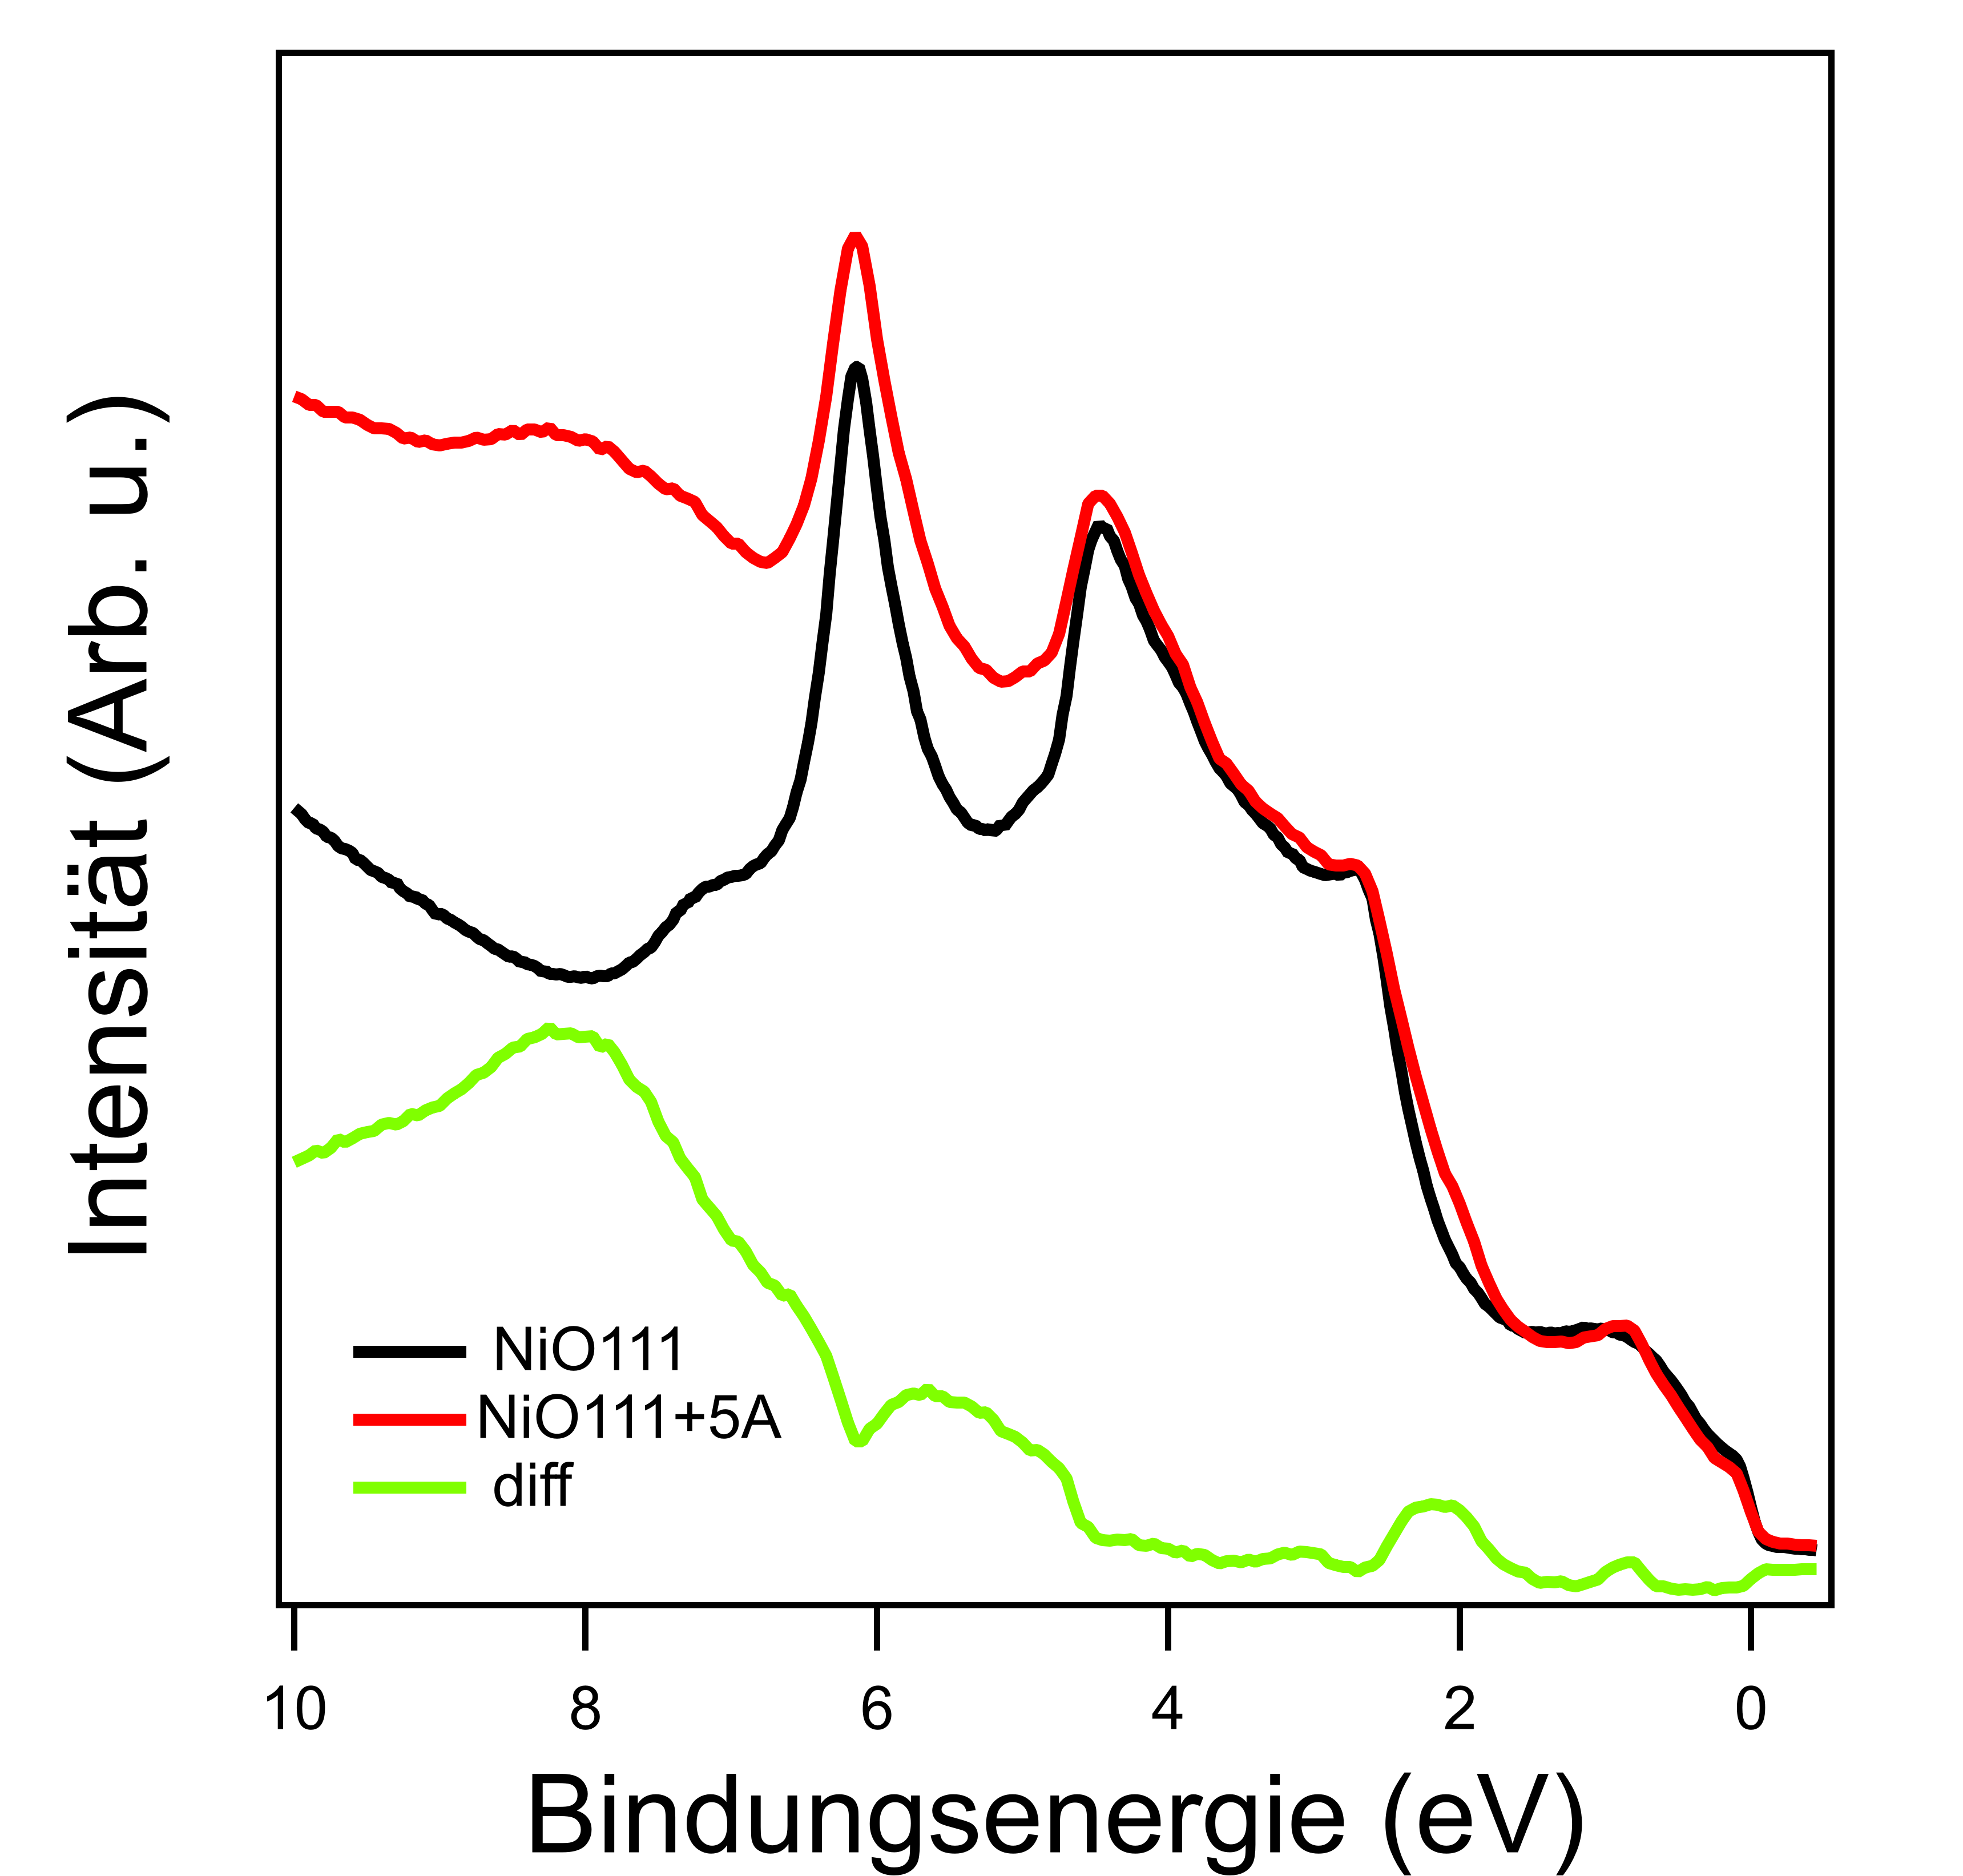
\includegraphics[height=4cm]{NiO+5A/EDC_NiO_thin_5A.png}
                    \subcaption{}
                    \label{fig:EDC_NiO_thin+5A}
                \end{subfigure}
                \begin{subfigure}[t]{0.30\textwidth}
                    \centering
                    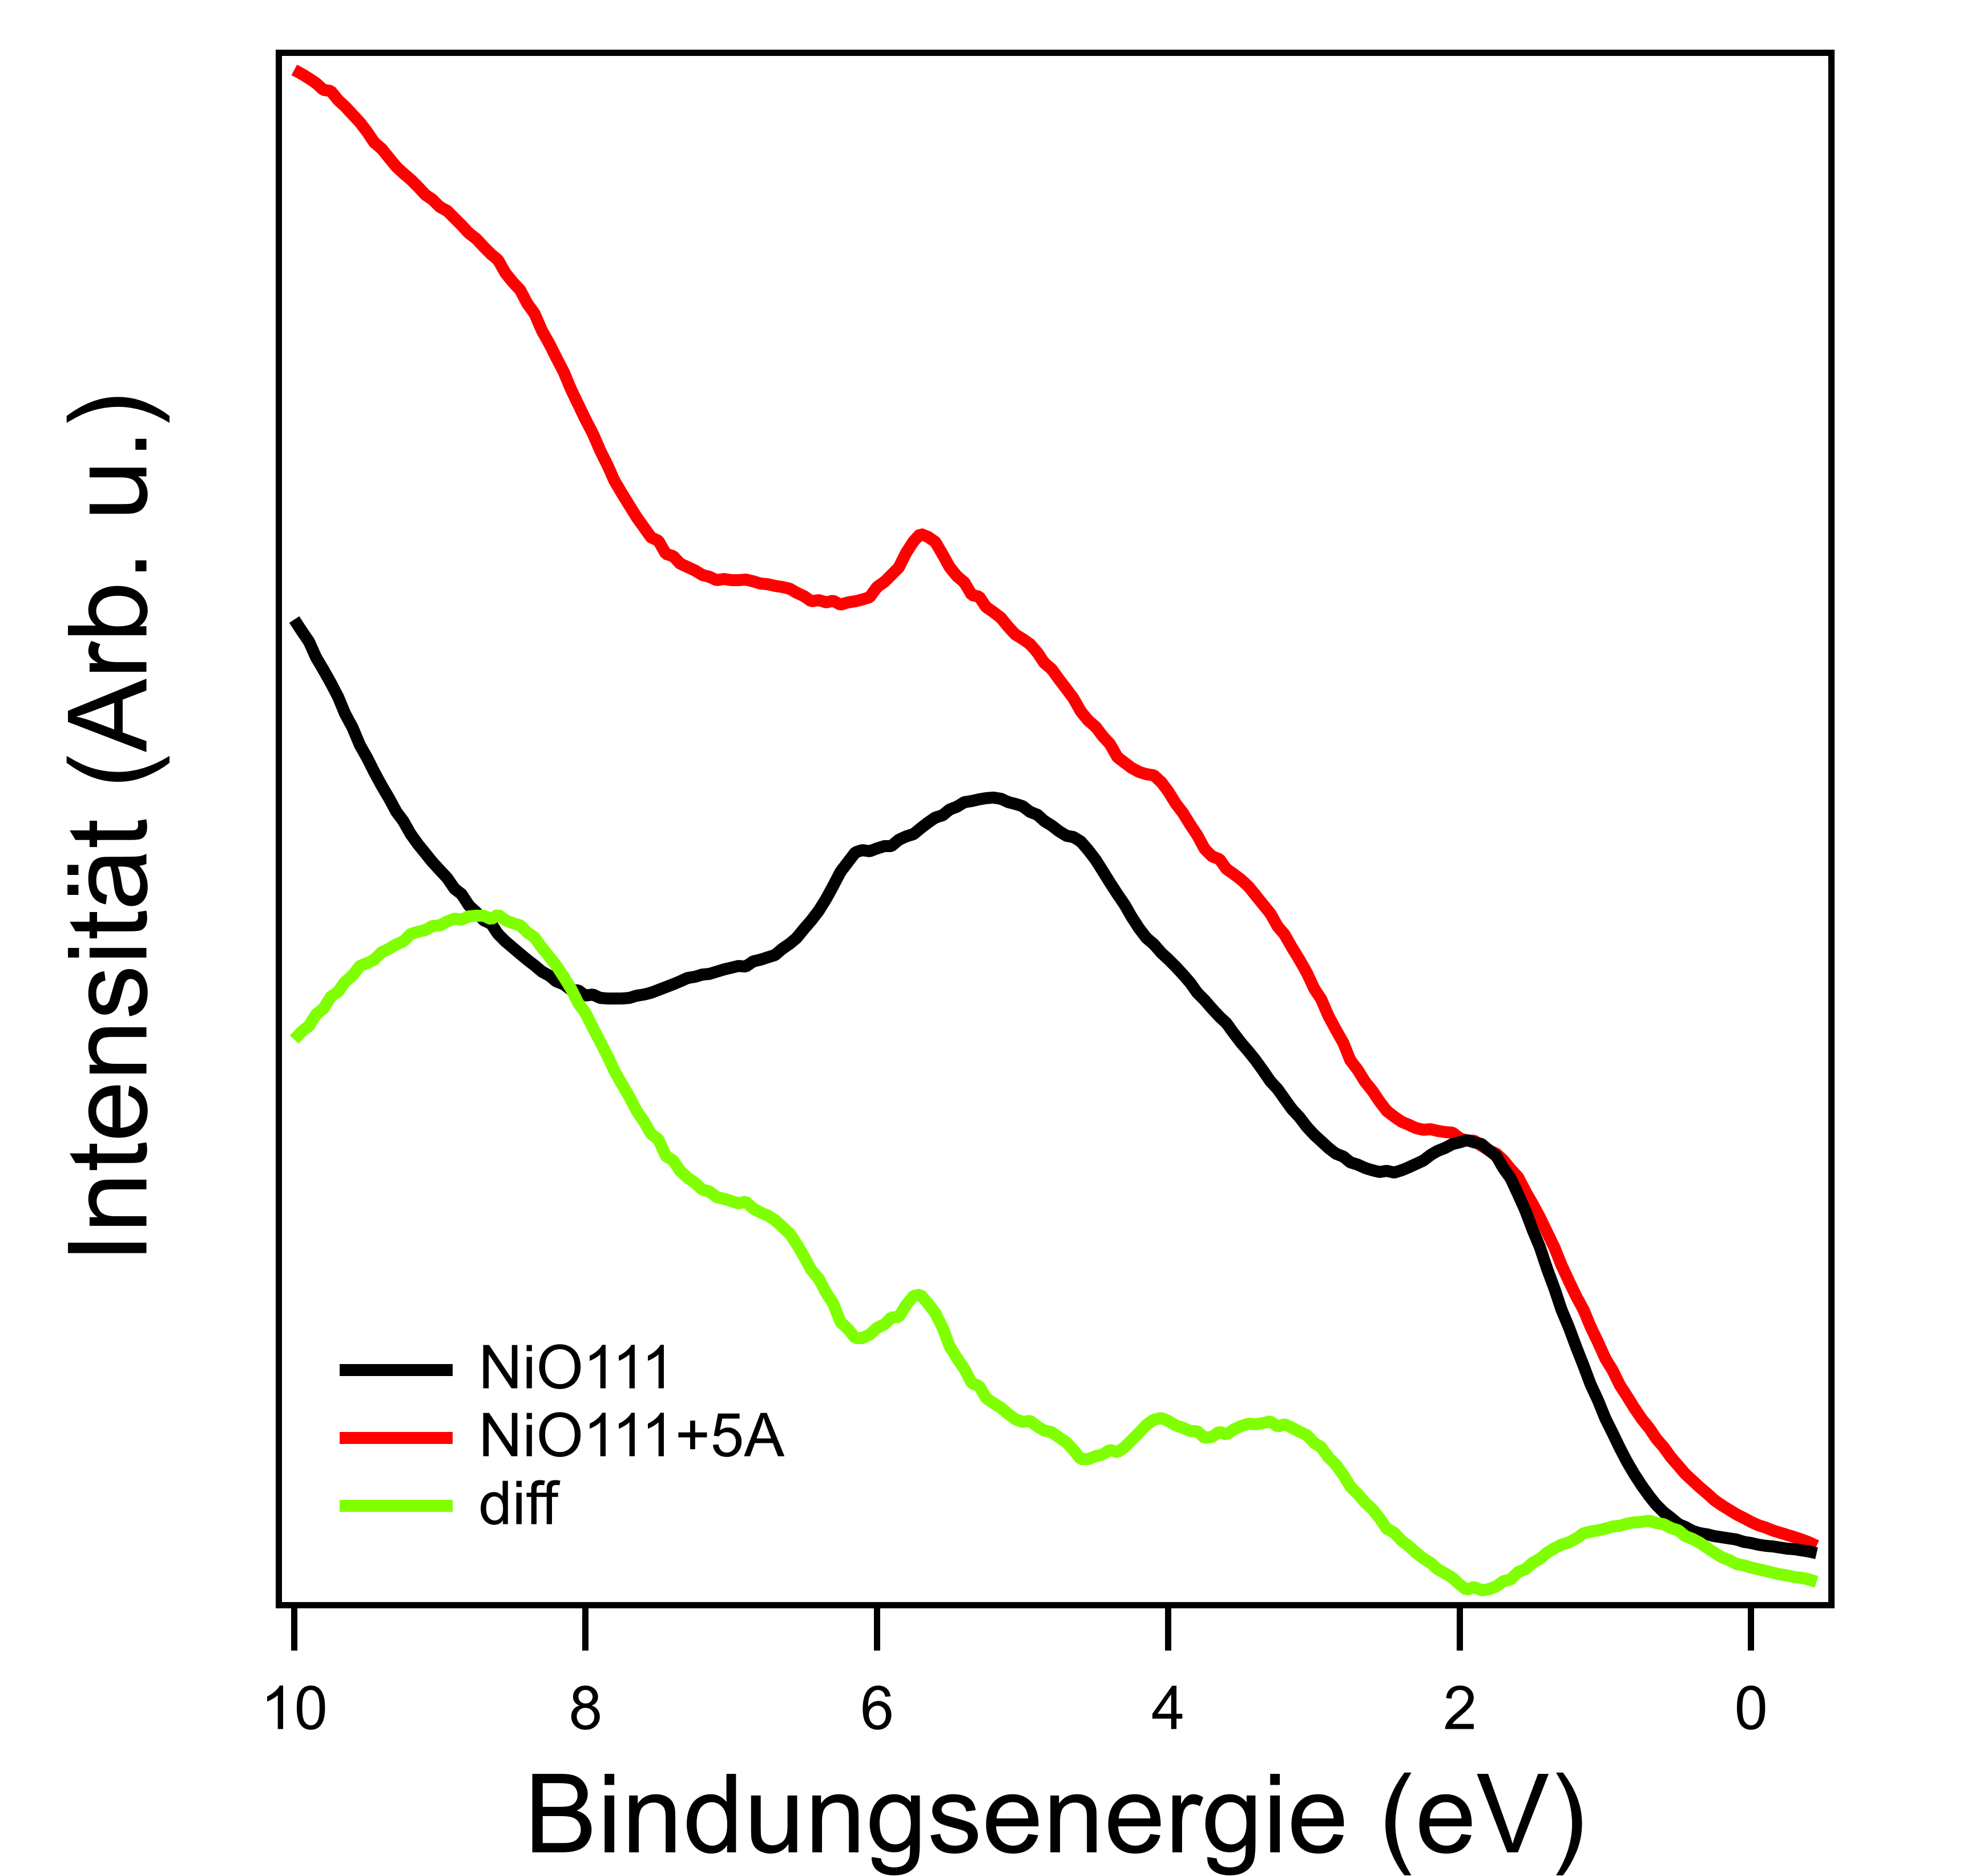
\includegraphics[height=4cm]{NiO+5A/NiO_5A_thick_new.png}
                    \subcaption{}
                    \label{fig:EDC_NiO+5A}
                \end{subfigure}
                \caption{Valenzbandspektrum des reinen Substrates (schwarz) und mit einer Monolage Pentacen bedeckt (rot) und dessen Differenz (grün).
                In (\subref{fig:EDC_Au+5A}) für \ce{Au}(111), in (\subref{fig:EDC_NiO_thin+5A}) für den dünnen Nickeloxidfilm und für den dicken Nickeloxidfilm in (\subref{fig:EDC_NiO+5A}).}
            \end{figure}
            Mit wachsender Schichtdicke des Nickeloxides auf der Goldoberfläche und jeweils mit Pentacen zeigen sich besonders im Bereich bis \SI{3}{\electronvolt} Veränderungen im winkelintegrierten Valenzbandspektrum.
            So ist für das Gold bei etwa \SI{1}{\electronvolt} der Beitrag des HOMO und bei etwa \SI{2}{\electronvolt} der Beitrag des HOMO-1 zu erkennen.
            Bestätigen lässt sich dies mittels der winkelaufgelösten Bildern der Photoemissionsorbitaltomographie.
            Wie für adsorbierte Moleküle erwartet, sind die Strukturen in der EDC eher breit, da die Lebenszeit der Zustände verkürzt und damit die Energieniveaus aufgeweitet werden.
            Auch bei den dünnen Nickeloxidfilm sind noch Beiträge der Molekülzustände nahe der Fermikante zu erkennen, wohingegen die Beiträge bei dem dickeren Film verschwinden.
            Für alle zeigt sich allerdings deutlich noch ein weiteres Signal bei \SI{8}{\electronvolt}, welches von einem höherliegendem Molekülorbital herrührt.
            Beim dickeren Nickeloxid ist dies sogar etwa weiter zu höheren Bindungsenergien verschoben.
            Ebenso taucht ein neuer Beitrag bei etwa \SI{6}{\electronvolt} auf.
            Es deutet darauf hin, dass die Interaktion bei dem dicken Nickeloxidfilm stärker ist.
            Besonders die äußeren Molekülorbitale mit einer geringen Bindungsenergie werden verändert oder nicht mehr besetzt.
            Auch die Adsorption auf unterschiedlichen Plätzen und Orientierungen kann eine Ursache für diesen Effekt sein.
            Hier kann sich die Wechselwirkung mit dem Substrat unterschiedlich äußern und damit die Lage der Molekülniveaus unterschiedliche Werte annehmen.

            \begin{figure}
                \centering
                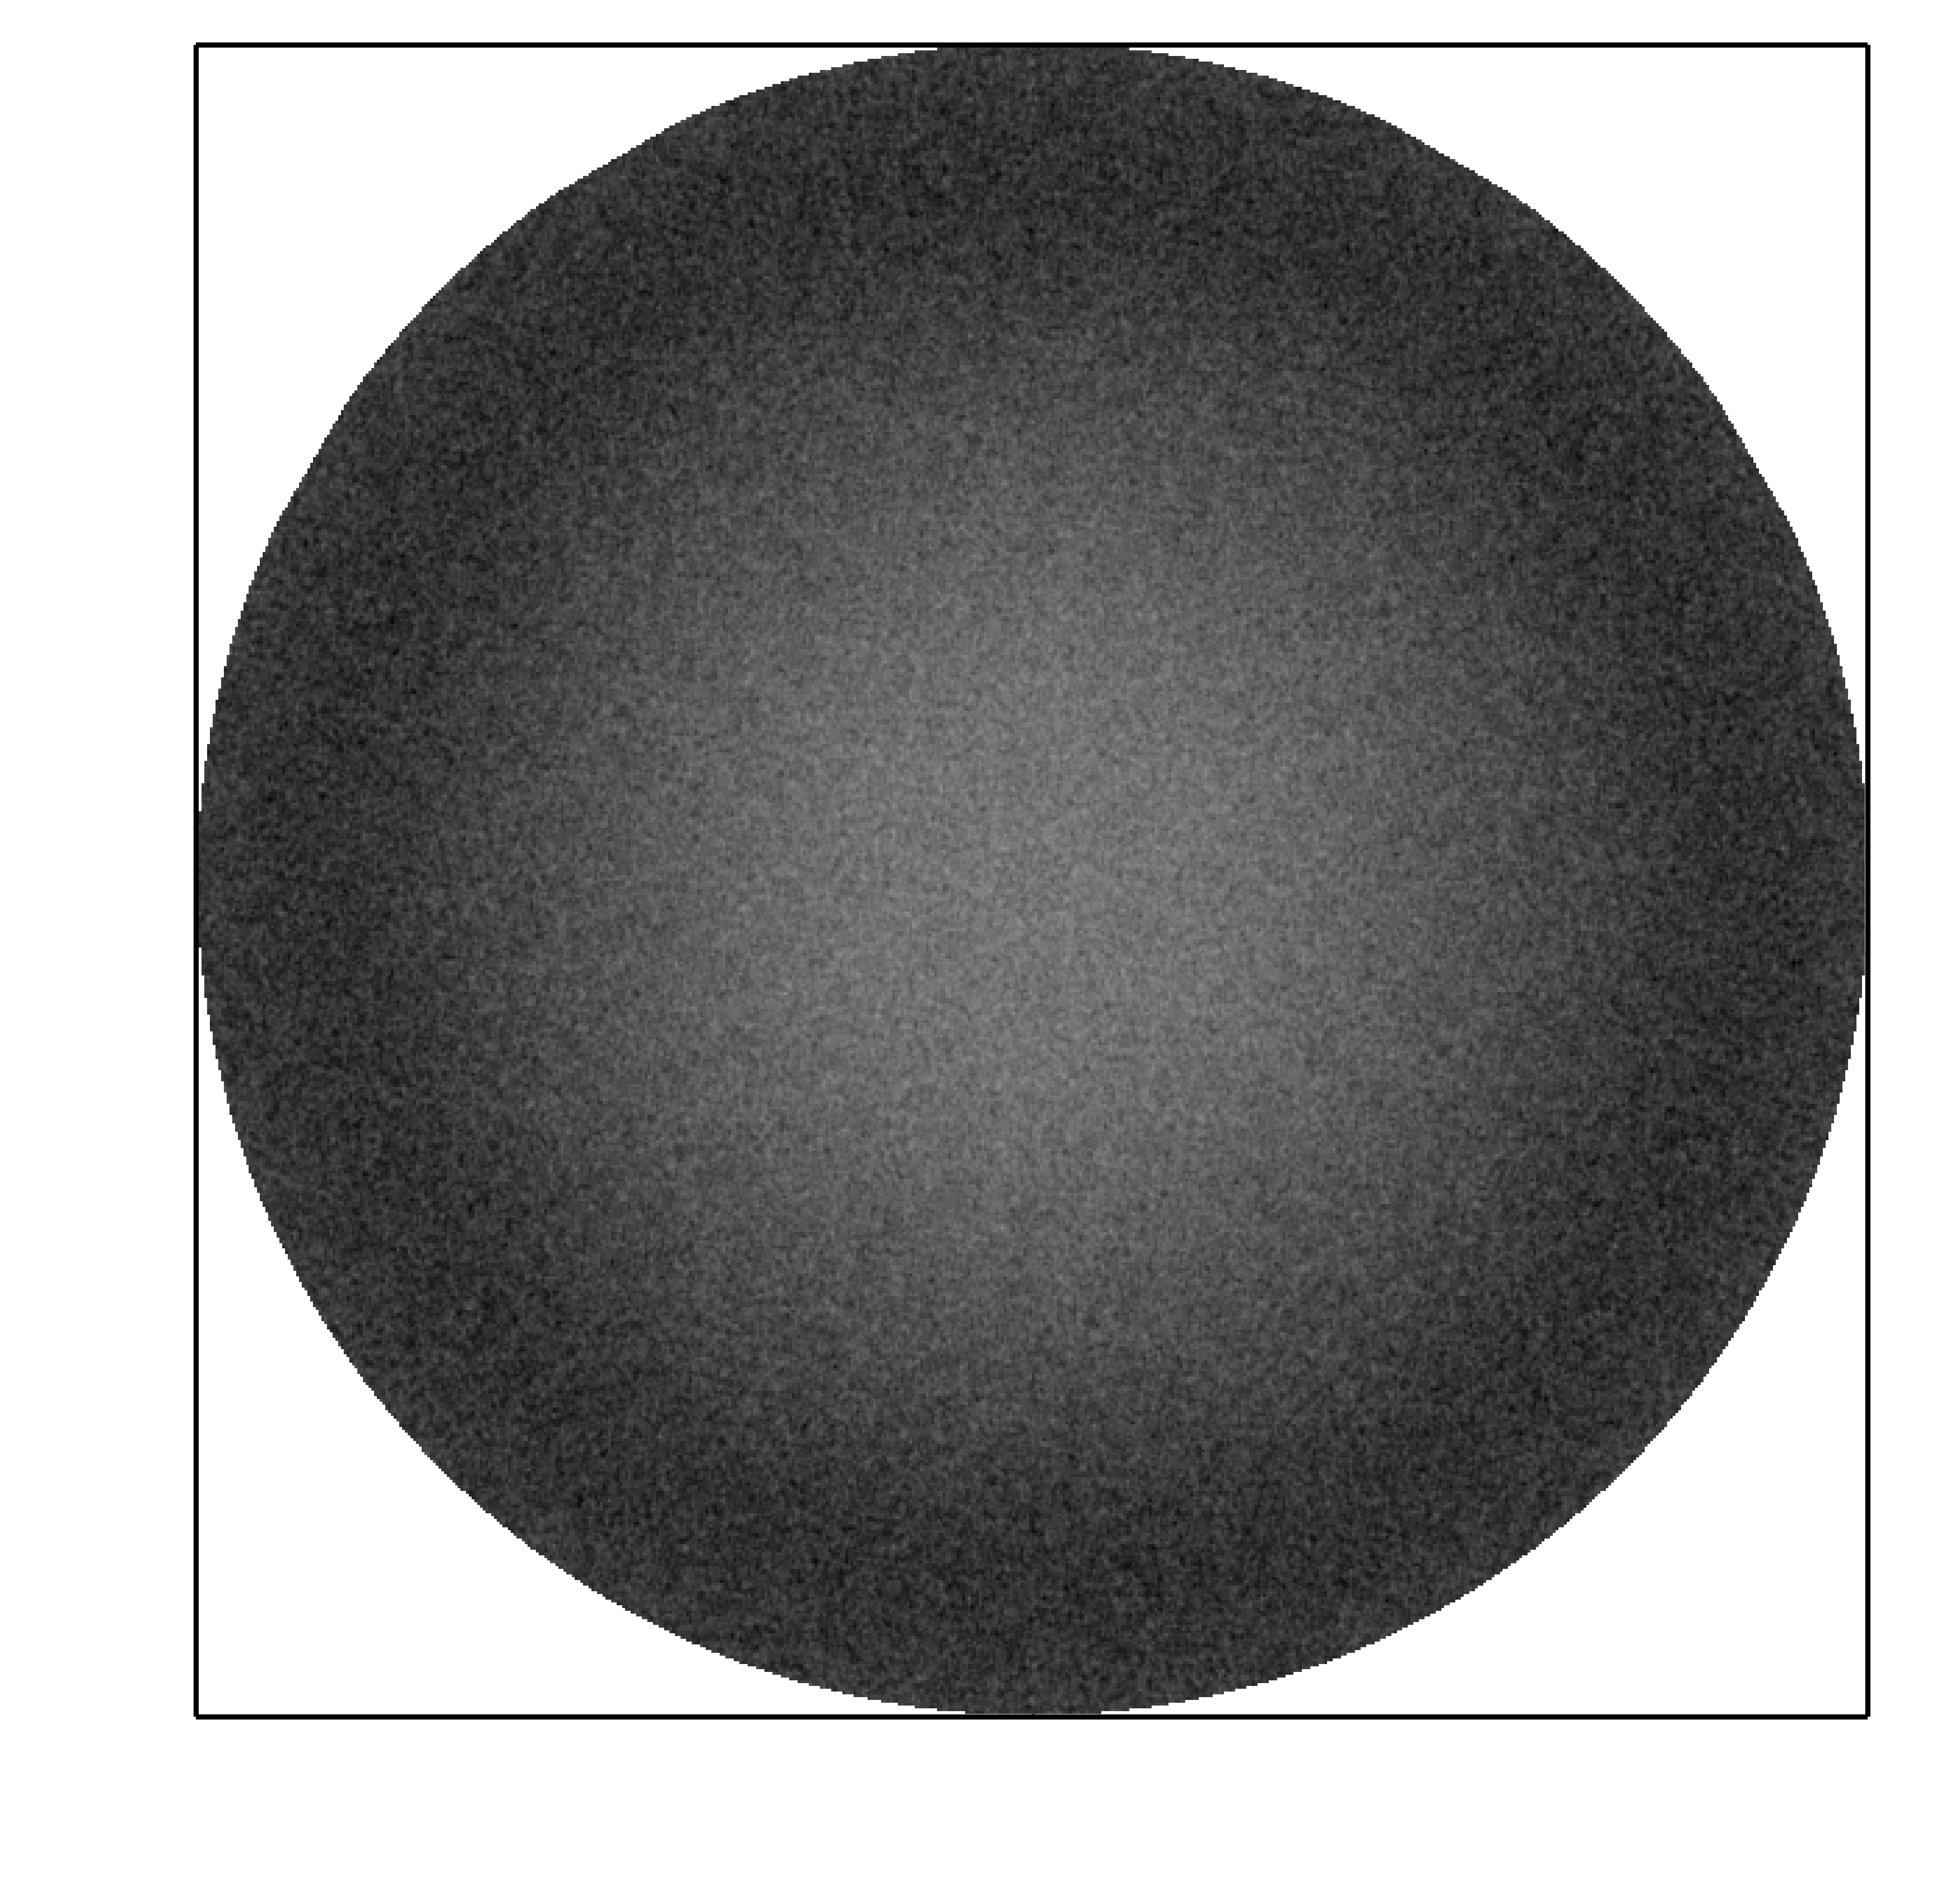
\includegraphics[height=5cm]{NiO+5A/NiO_thick_5A_KE12_7.png}
                \caption{Das winkelaufgelöste Bild bei einer Bindungsenergie von \SI{3.85}{\electronvolt} für Pentacen auf dem dicken Nickeloxidfilm.} % bei einer kinetischen Energie von \SI{7.5}{\electronvolt}. Also Bindungsenergie von \SI{3.85}{\electronvolt}.
                \label{fig:MOT_NiO+5A}
            \end{figure}
            Gleiches findet sich in den winkelaufgelösten Bildern wieder.
            Ein Beispiel ist in \autoref{fig:MOT_NiO+5A} zu sehen.
            Dieses Bild wurde gewählt da ein deutliches Signal im integrierten Spektrum zu erkennen ist.
            % Dabei zeigt der direkte Vergleich der integrierten Spektren in \autoref{fig:EDC_NiO+5A} des reinen Nickeloxid und des mit Pentacen drauf deutliche zusätzliche Spitzen.
            Die Abwesenheit sehr ausgeprägter Merkmale in den impulsaufgelösten Bildern bestätigt die Annahme, dass sich die Moleküle auf der Oberfläche nicht regelmäßig anordnen.
            % Ferner überlappen die einzelnen Merkmale im Impulsraum, sodass ein ausgewaschenes Bild entsteht.
            % Wie bereits erwähnt sind vor allem in der Nähe der Fermikante im integrierten Spektrum in \autoref{fig:EDC_NiO} keine klaren Unterschiede aufgezeigt.
            % Das sich die Moleküle nicht auf der Oberfläche ordnen kann die Ursache von zu starker oder zu schwacher Wechselwirkung sein.
            % Da sich auf der Oberfläche der (111)-Orientierung des Nickeloxid auf Grund der Polarität ein Dipolmoment ausbildet, führt dies zu einer stärkeren Wechselwirkung.
            % Liegt die Oberfläche auch noch in der \ce{O} beziehungsweise \ce{OH-}-Terminierung vor so ist eine Abwesenheit von kovalenten Bindungen nicht auszuschließen.
            % Starke kovalente Bindungen, können wie bereits erwähnt die Selbstanordnung behindern (s. \autoref{sec:Selbstanordnung}).
            % Vermutlich handelt es sich um den Effekt der zu starken Wechselwirkung, da sich dann die Pentacen Moleküle nicht ordnen.
            Eine Ordnung der Moleküle findet vermutlich aufgrund der instabilen und imperfekten Oberfläche nicht statt.
            % Allerdings kann anderenfalls die Ausbildung von verschiedenen Domänen und Orientierungen entlang der Substratachsen zu einer Verschmierung in der Winkelauflösung führen~\cite{scholl_chapter_2018}.
            Weiter verschiebt sich die Austrittsarbeit beim mit Pentacen bedampften dünnen Nickeloxidfilm zu einem Wert von \SI{4.14}{\electronvolt}.
            Dies ist eine Verschiebung um \SI{0.11}{\electronvolt} hinsichtlich dem dünnen Nickeloxidfilm.
            Dieser Effekt wird erwartet, da durch den Push-Back-Effekt die Austrittsarbeit verringert wird.

        \FloatBarrier
        \subsection{Pentacen auf Eisenmonooxid}
            Im Gegensatz zu dem Nickeloxid zeigt das Wüstit trotz der Abwesenheit eines klaren Beugungsbildes ausgeprägte Merkmale in den winkelaufgelösten Messungen.
            Diese Merkmale können sich nur ausbilden, wenn sich die Moleküle regelmäßig und in gleicher Orientierung anordnen.
            \begin{figure}
                \centering
                \begin{subfigure}[t]{0.48\textwidth}
                    \centering
                    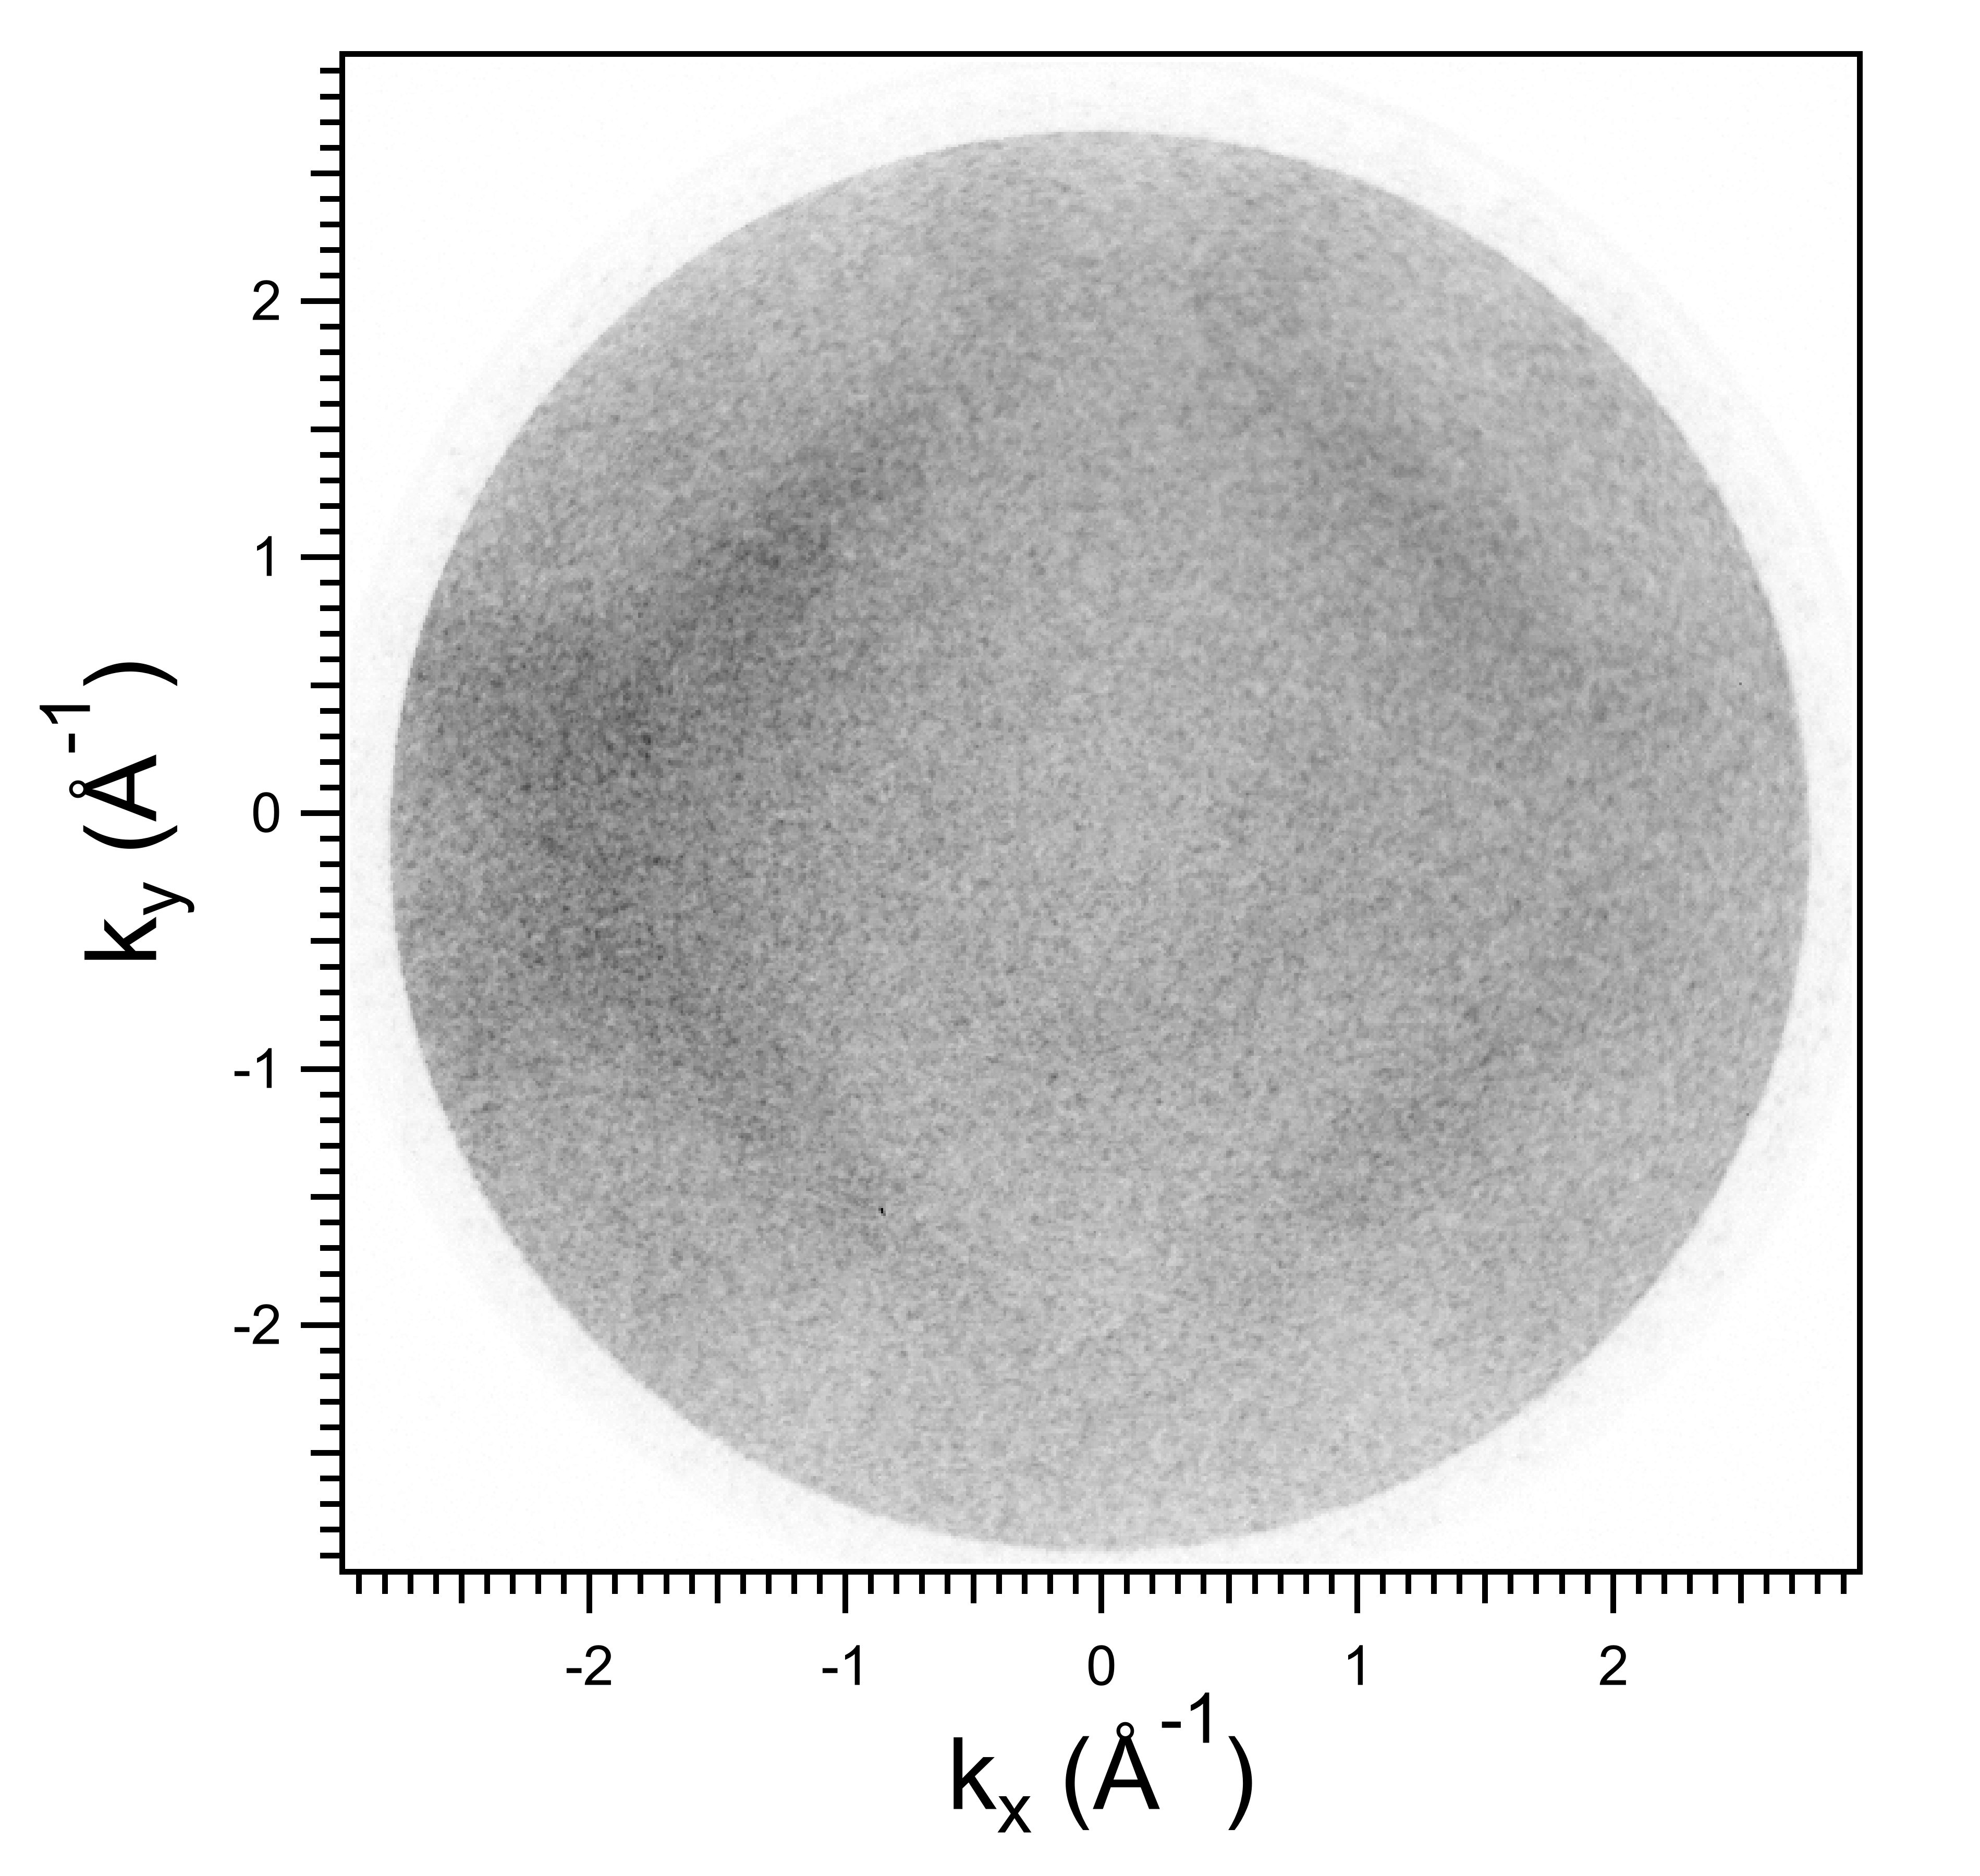
\includegraphics[height=3.7cm]{FeO+5A/FeO_5A_34_80eV.png}
                    \subcaption{\SI{0.70}{\electronvolt}}
                    % Das Bild für eine kinetische Energie von \SI{34.80}{\electronvolt}, also \SI{0.70}{\electronvolt} Bindungsenergie.
                    \label{fig:MOT_FeO+5A_exp_1}
                \end{subfigure}
                \begin{subfigure}[t]{0.48\textwidth}
                    \centering
                    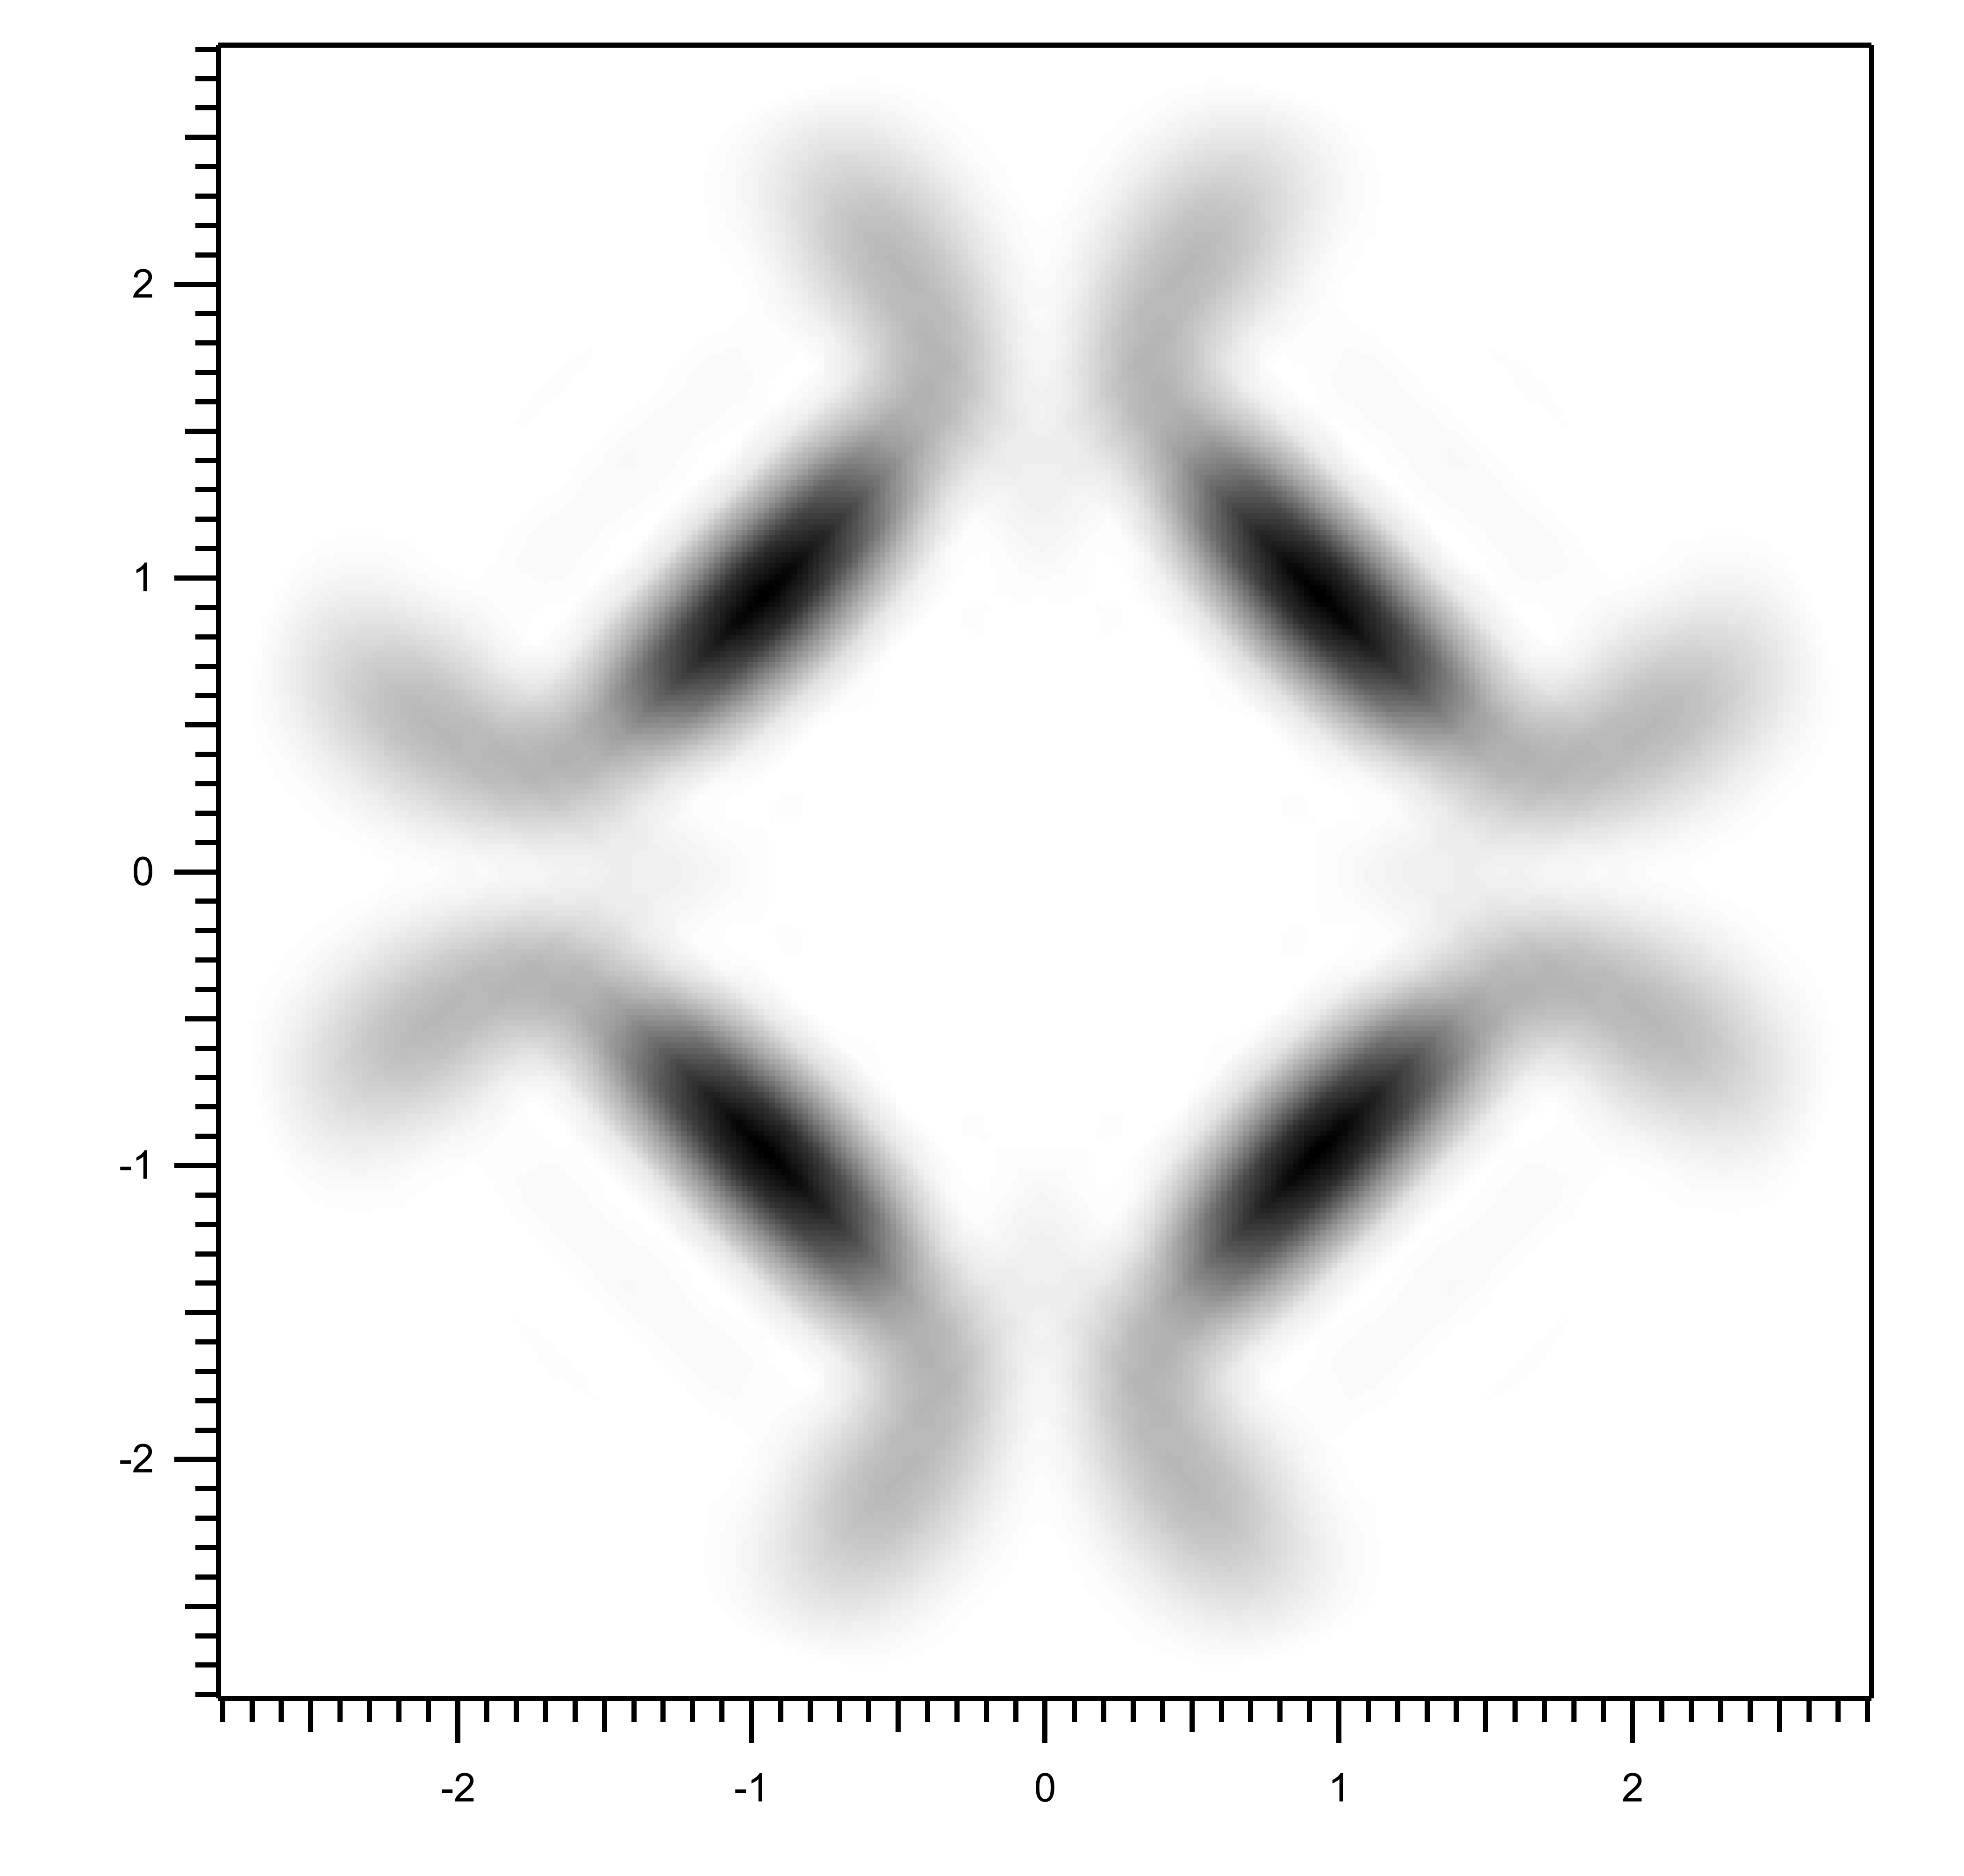
\includegraphics[height=3.7cm]{FeO+5A/MO_LUMO_RT_RT.png}
                    \subcaption{LUMO}
                    % Das LUMO mit Symmetrisierung zweier um \SI{90}{\degree} verdrehten Übergitter.
                    \label{fig:MOT_FeO+5A_theo_1}
                \end{subfigure}
                \centering
                \begin{subfigure}[t]{0.48\textwidth}
                    \centering
                    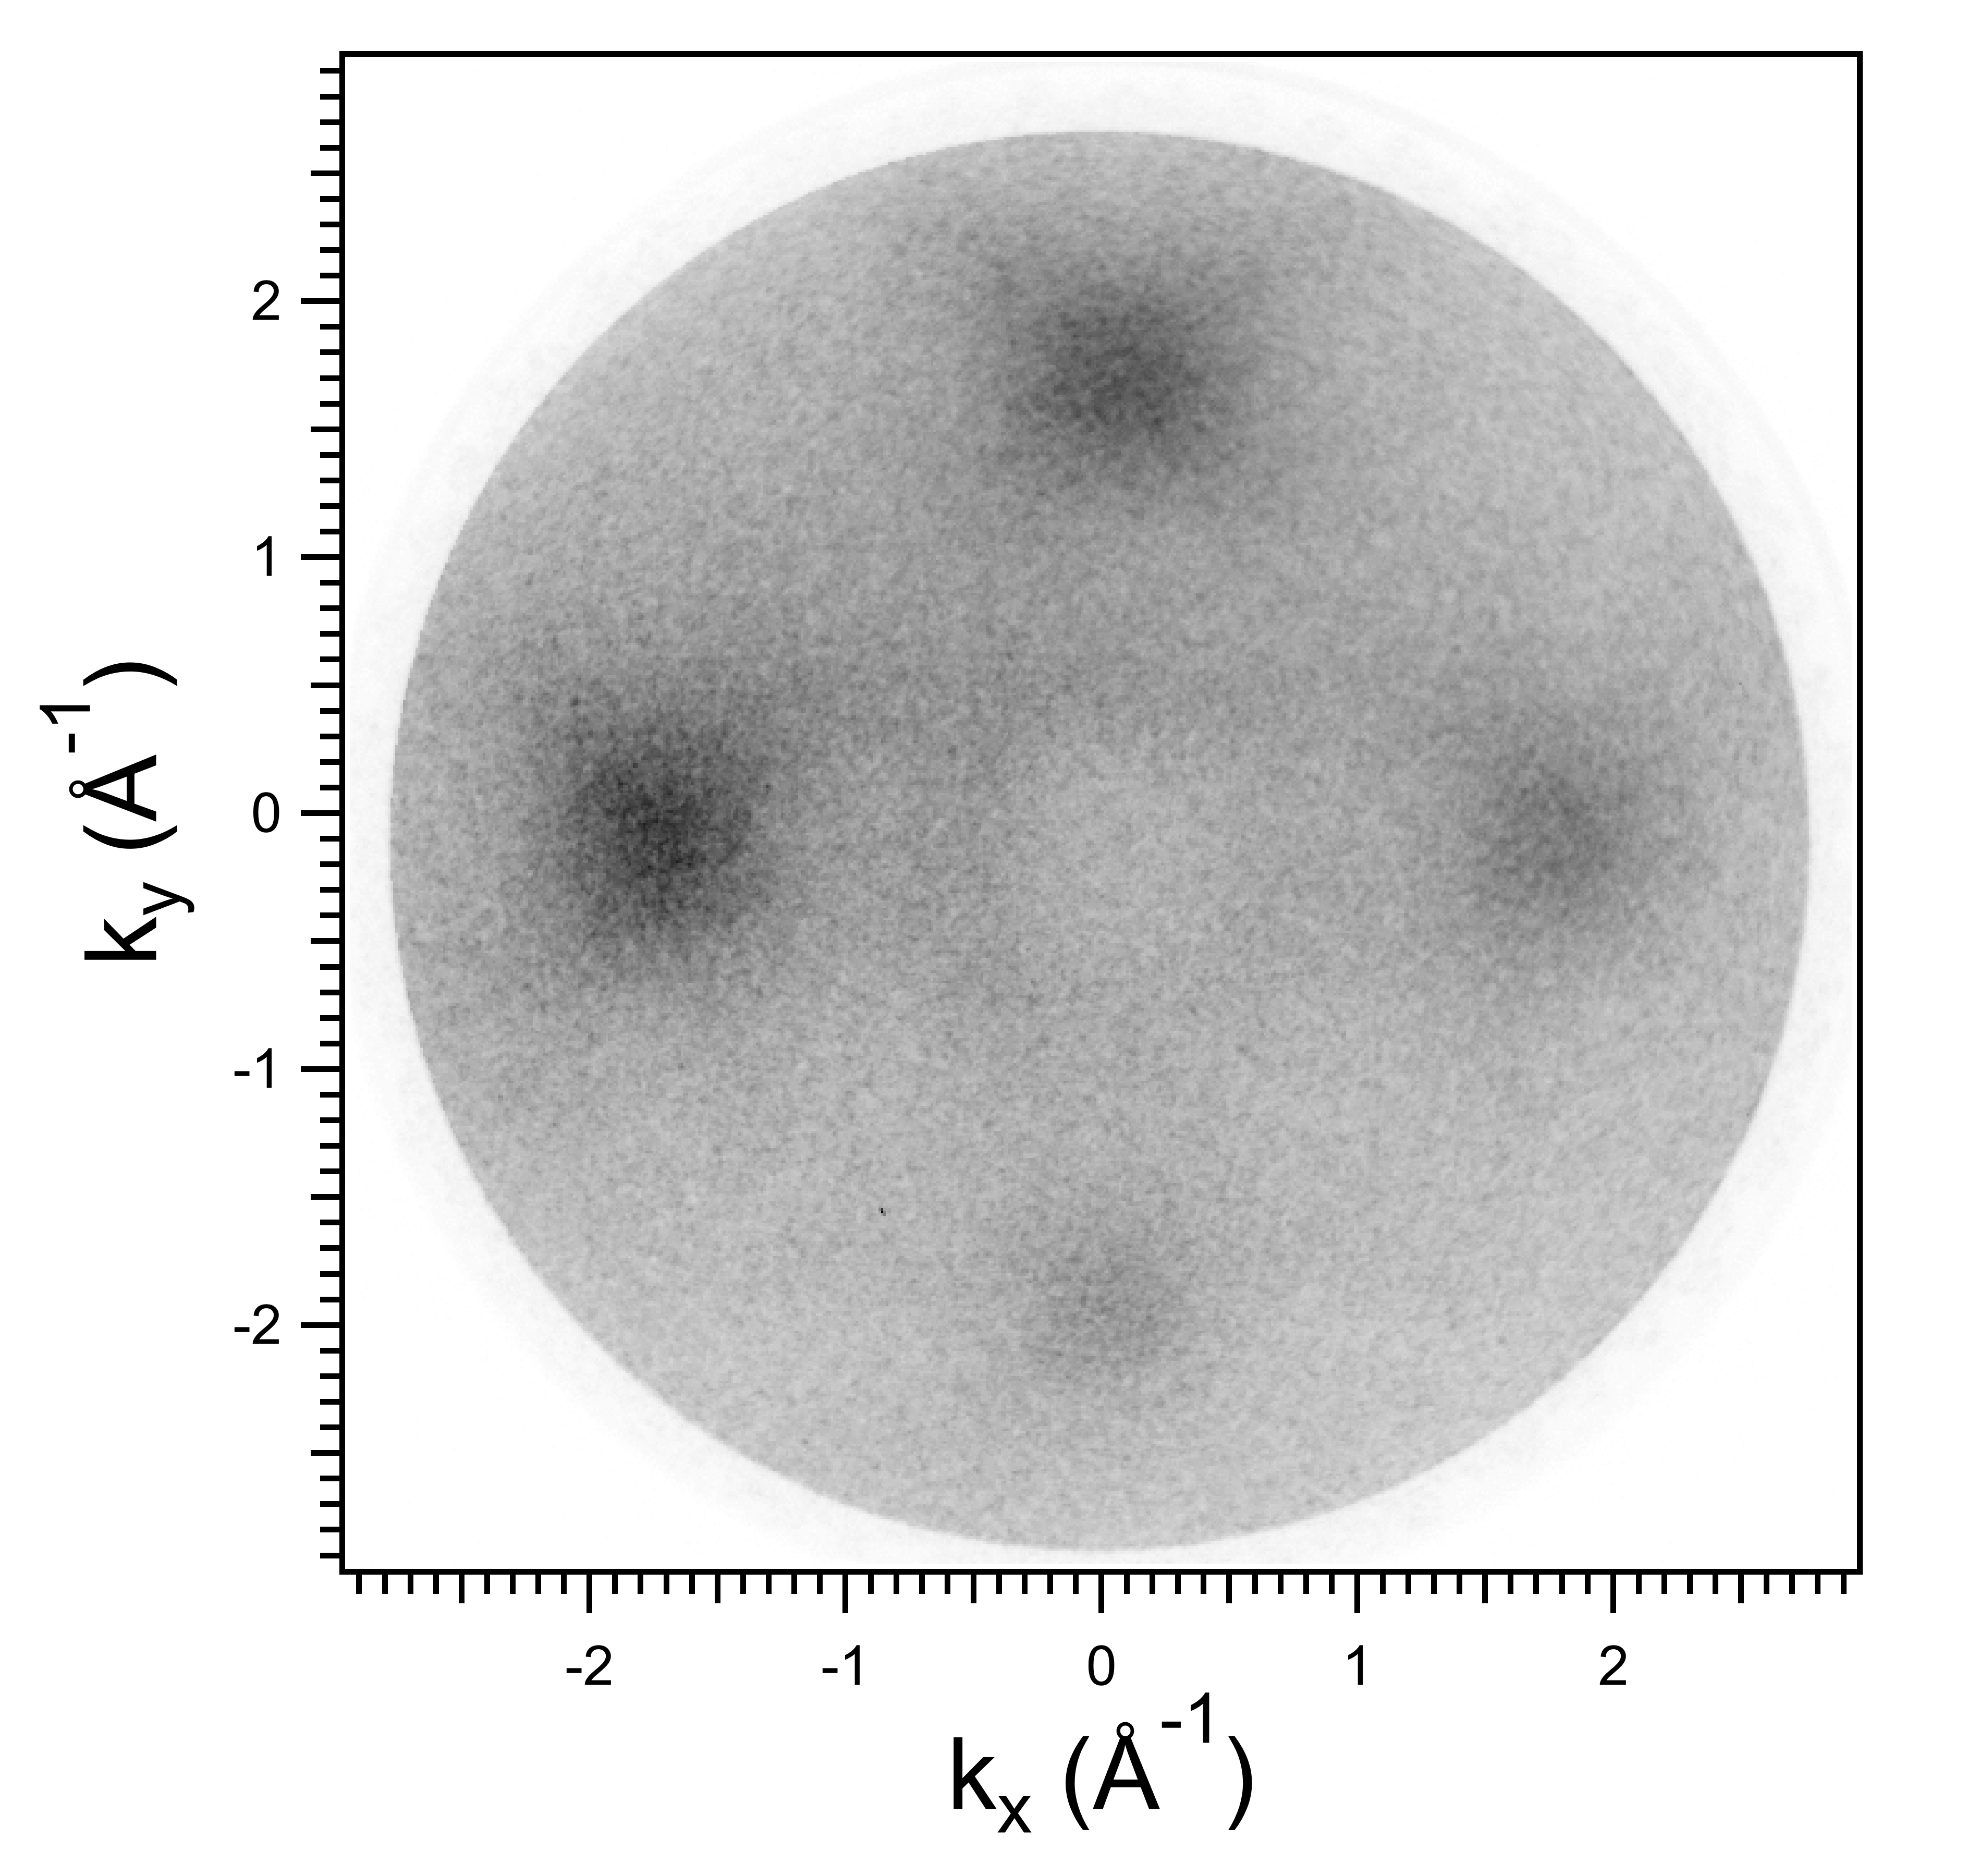
\includegraphics[height=3.7cm]{FeO+5A/FeO_5A_33_75eV.png}
                    \subcaption{\SI{1.75}{\electronvolt}}
                    % Das Bild für eine kinetische Energie von \SI{33.75}{\electronvolt}, also \SI{1.75}{\electronvolt} Bindungsenergie.
                    \label{fig:MOT_FeO+5A_exp_2}
                \end{subfigure}
                \begin{subfigure}[t]{0.48\textwidth}
                    \centering
                    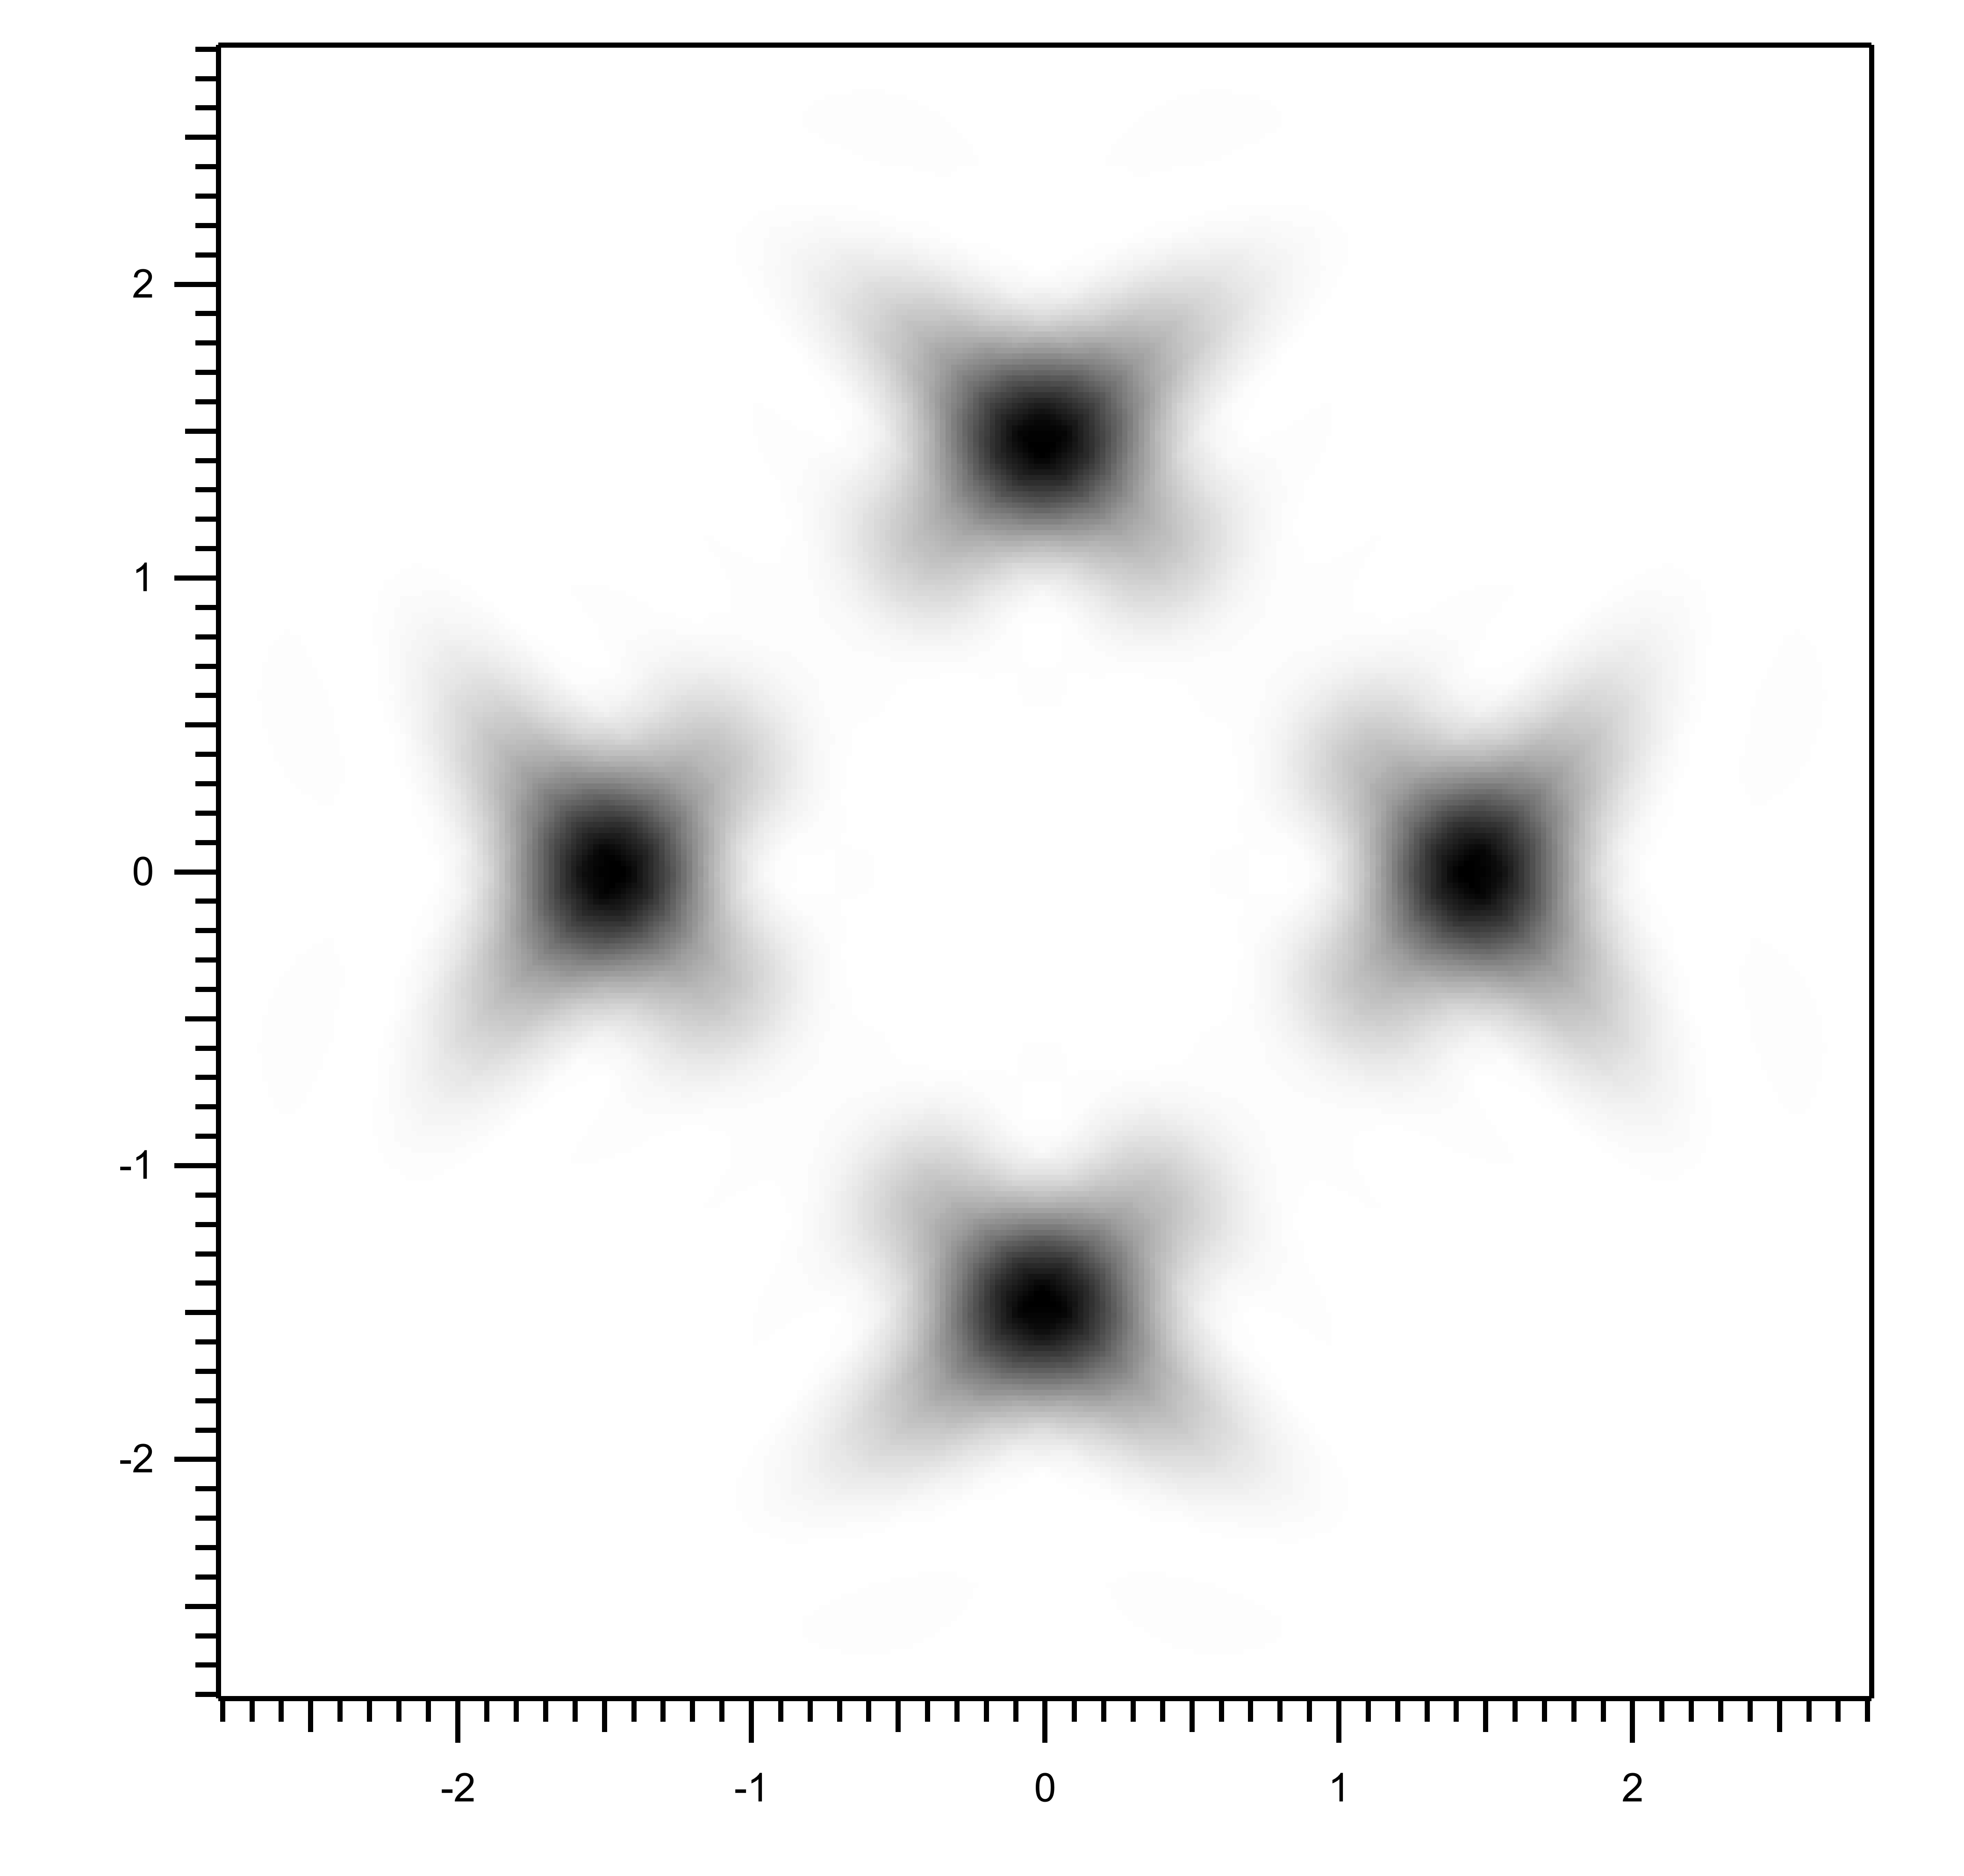
\includegraphics[height=3.7cm]{FeO+5A/MO_HOMO_RT_RT.png}
                    \subcaption{HOMO}
                    % Das HOMO mit Symmetrisierung zweier um \SI{90}{\degree} verdrehten Übergitter.
                    \label{fig:MOT_FeO+5A_theo_2}
                \end{subfigure}
                \centering
                \begin{subfigure}[t]{0.48\textwidth}
                    \centering
                    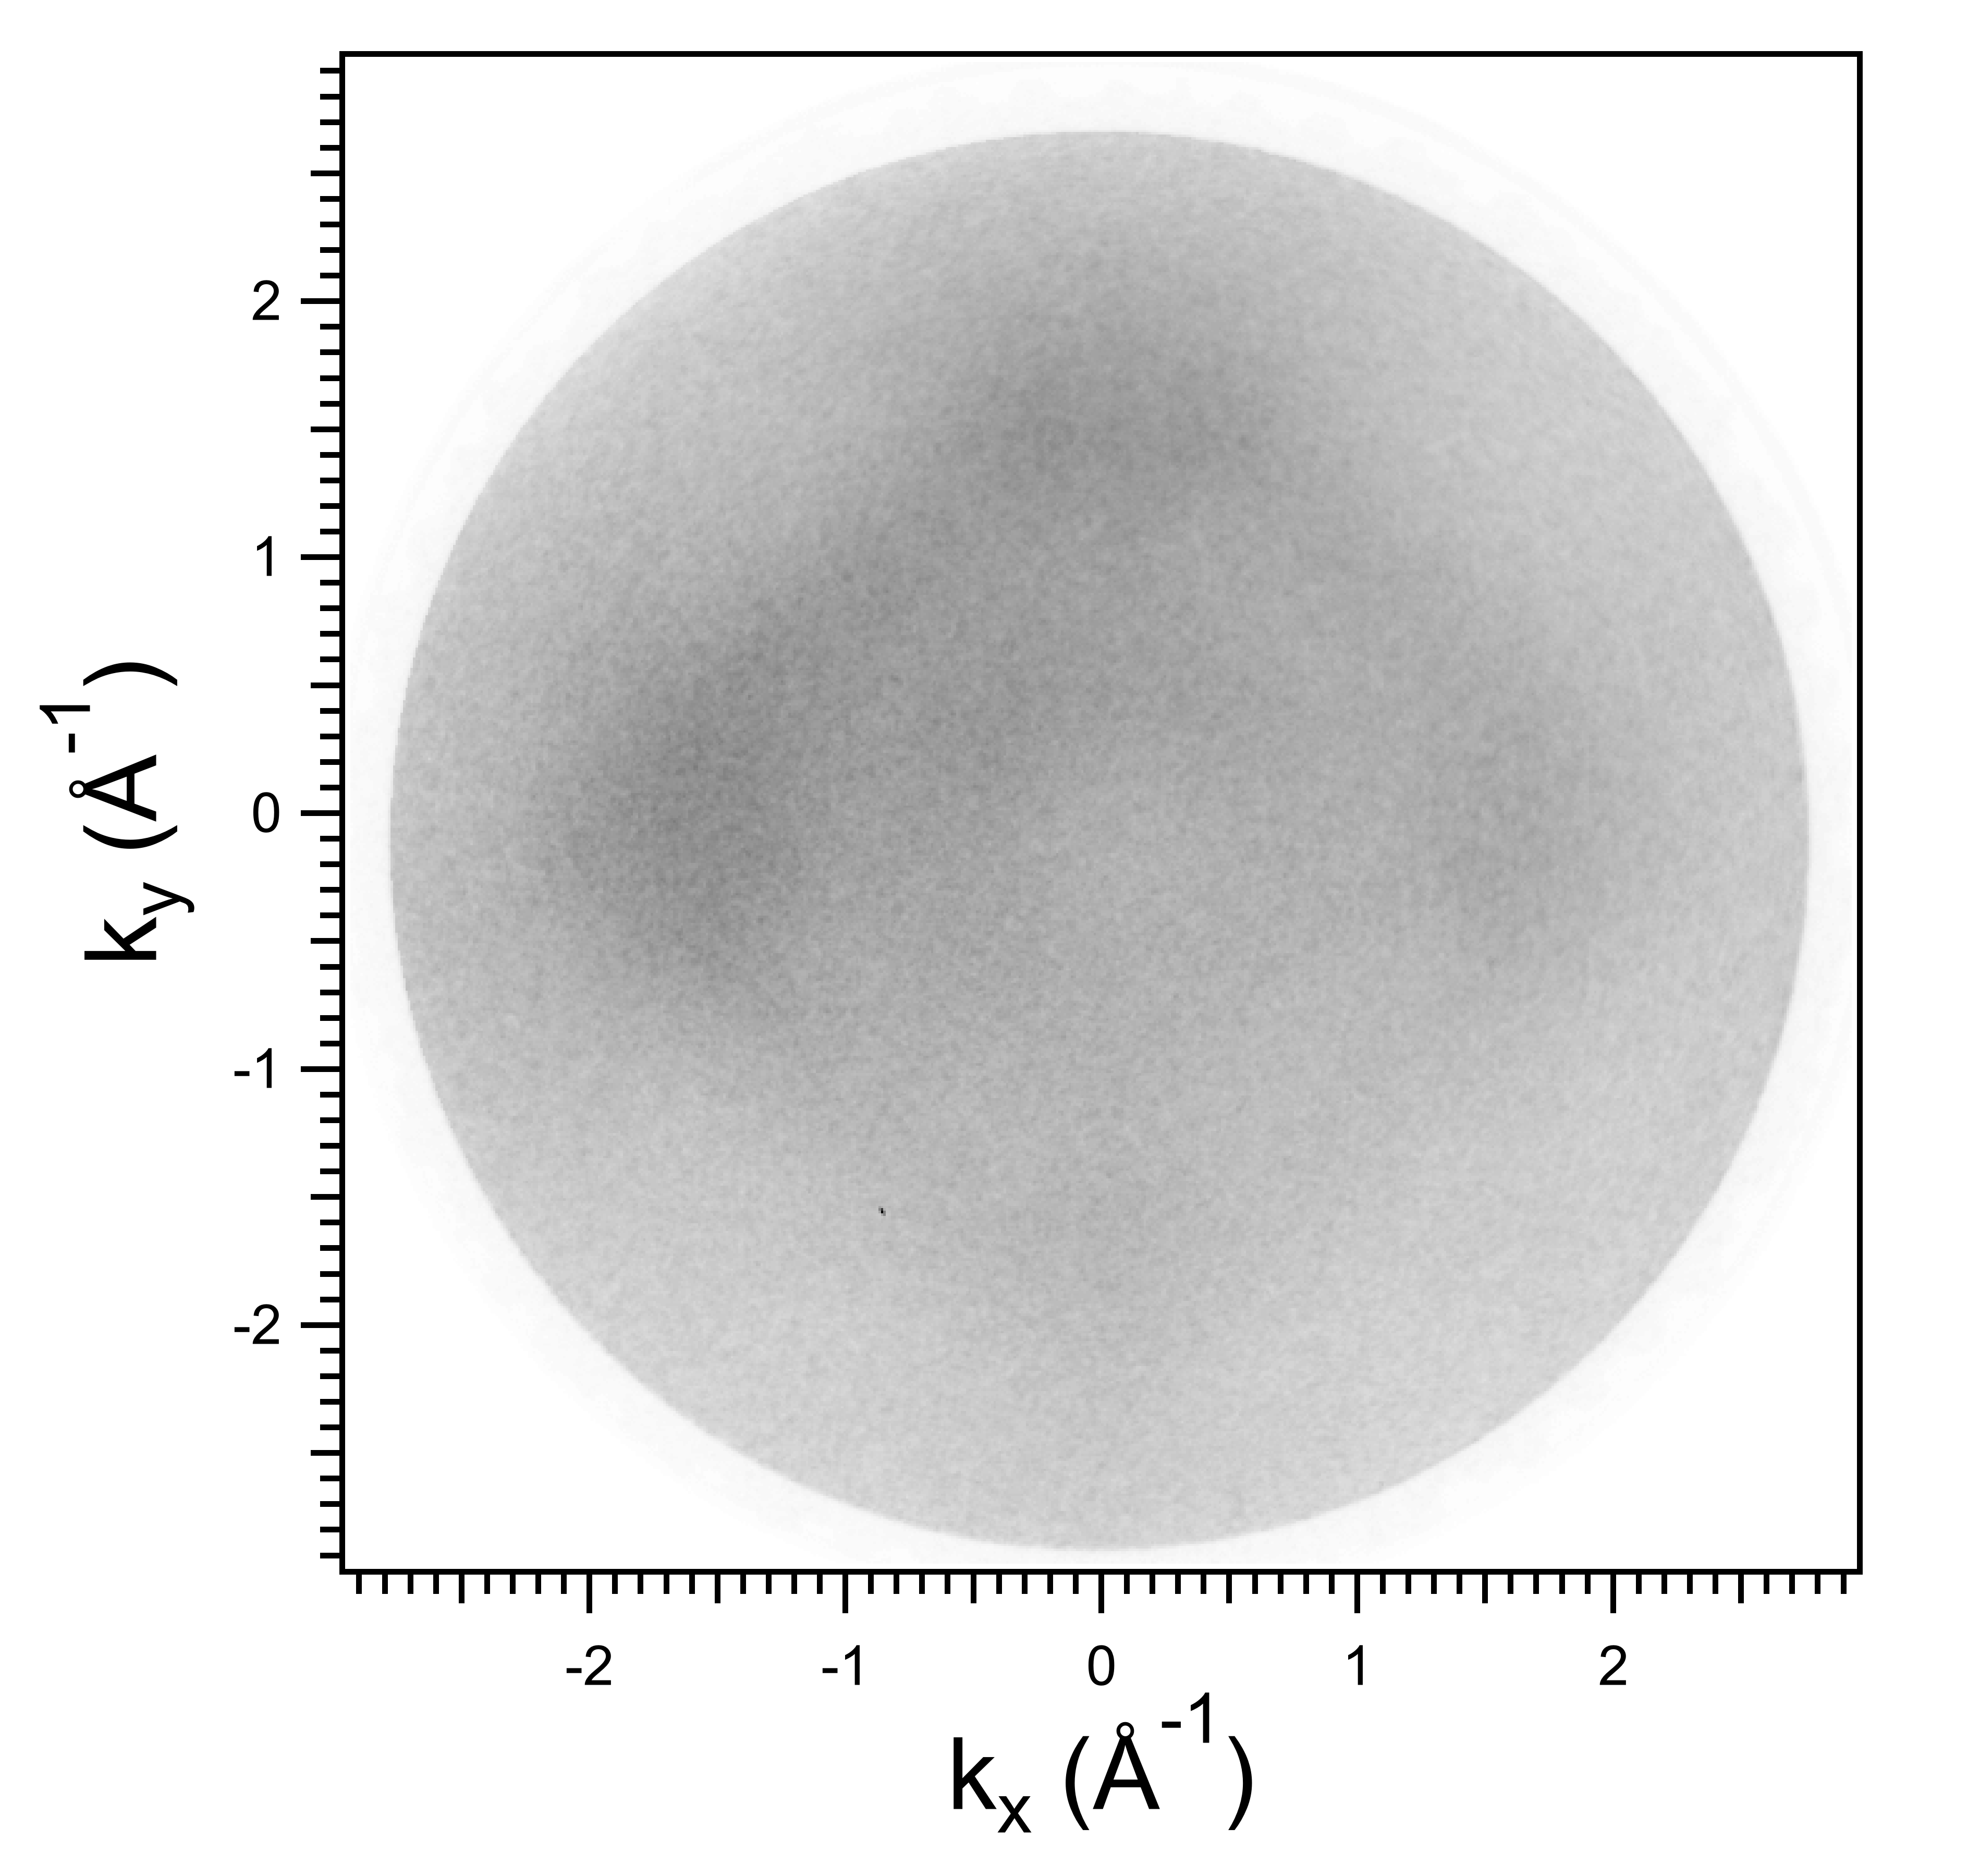
\includegraphics[height=3.7cm]{FeO+5A/FeO_5A_32_15eV.png}
                    \subcaption{\SI{3.35}{\electronvolt}}
                    % Das Bild für eine kinetische Energie von \SI{32.15}{\electronvolt}, also \SI{3.35}{\electronvolt} Bindungsenergie.
                    \label{fig:MOT_FeO+5A_exp_3}
                \end{subfigure}
                \begin{subfigure}[t]{0.48\textwidth}
                    \centering
                    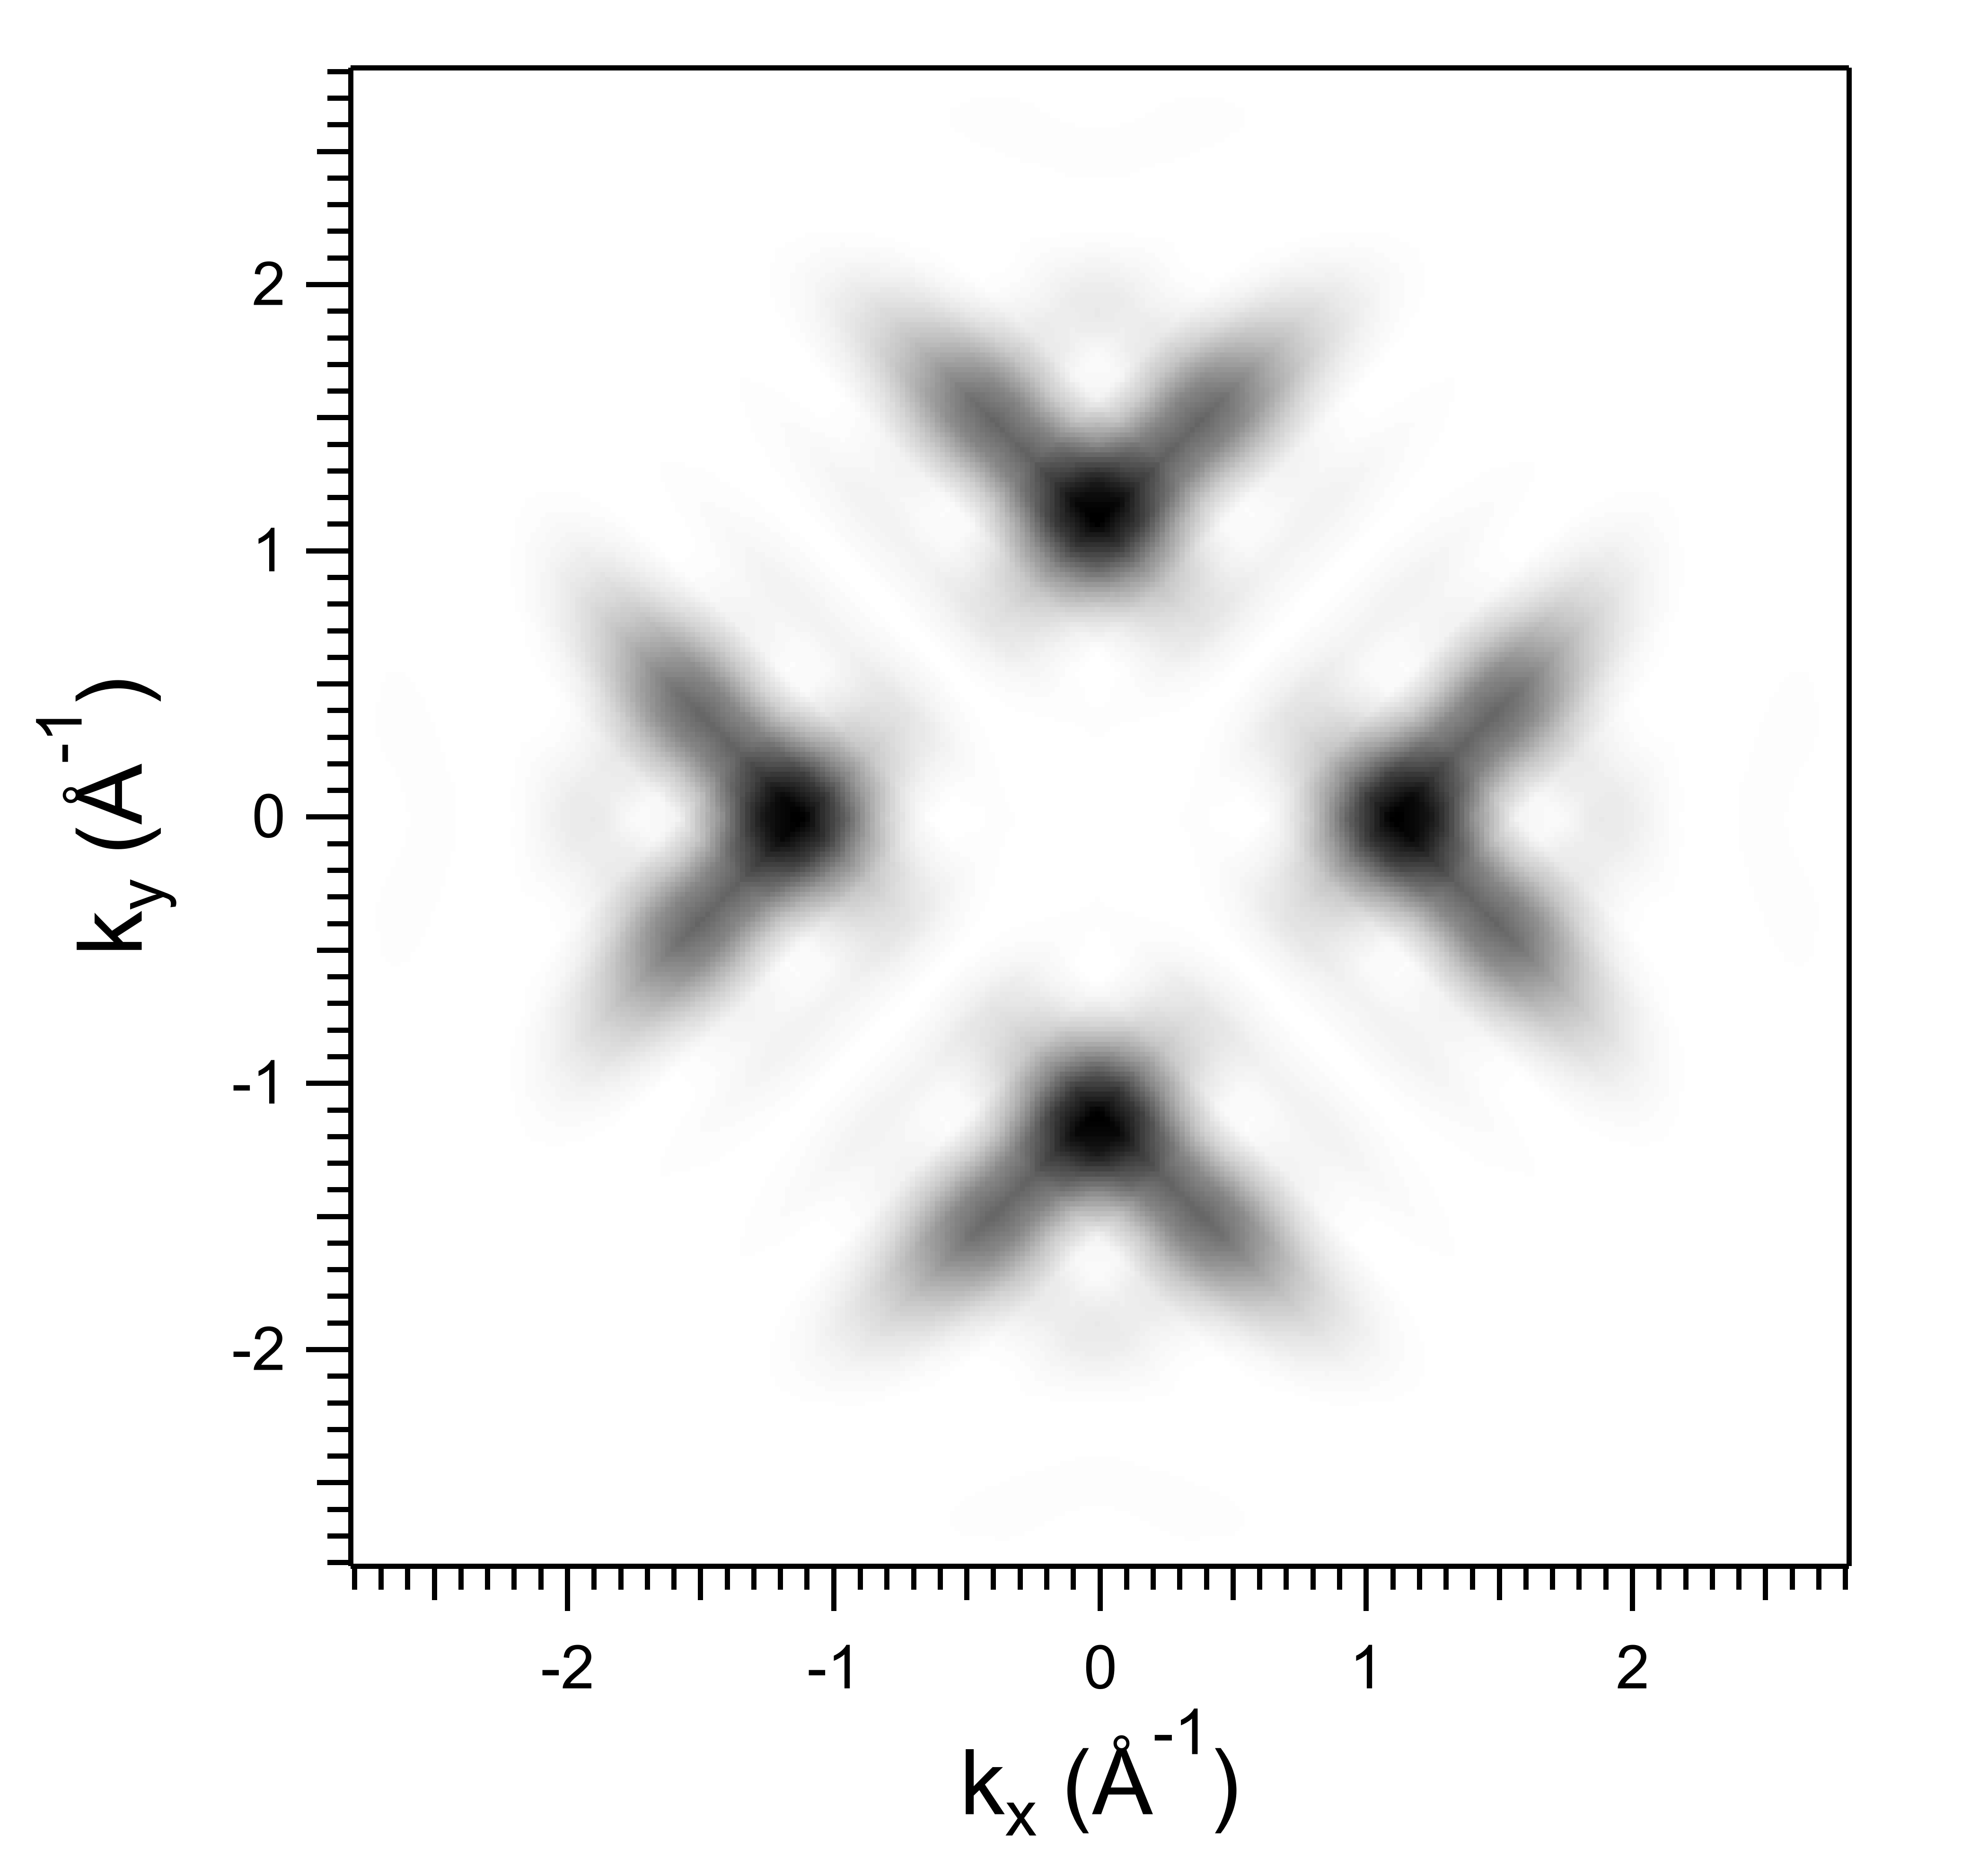
\includegraphics[height=3.7cm]{FeO+5A/MO_HOMO1_RT_RT.png}
                    \subcaption{HOMO-1}
                    % Das HOMO-1 mit Symmetrisierung zweier um \SI{90}{\degree} verdrehten Übergitter.
                    \label{fig:MOT_FeO+5A_theo_3}
                \end{subfigure}
                \centering
                \begin{subfigure}[t]{0.48\textwidth}
                    \centering
                    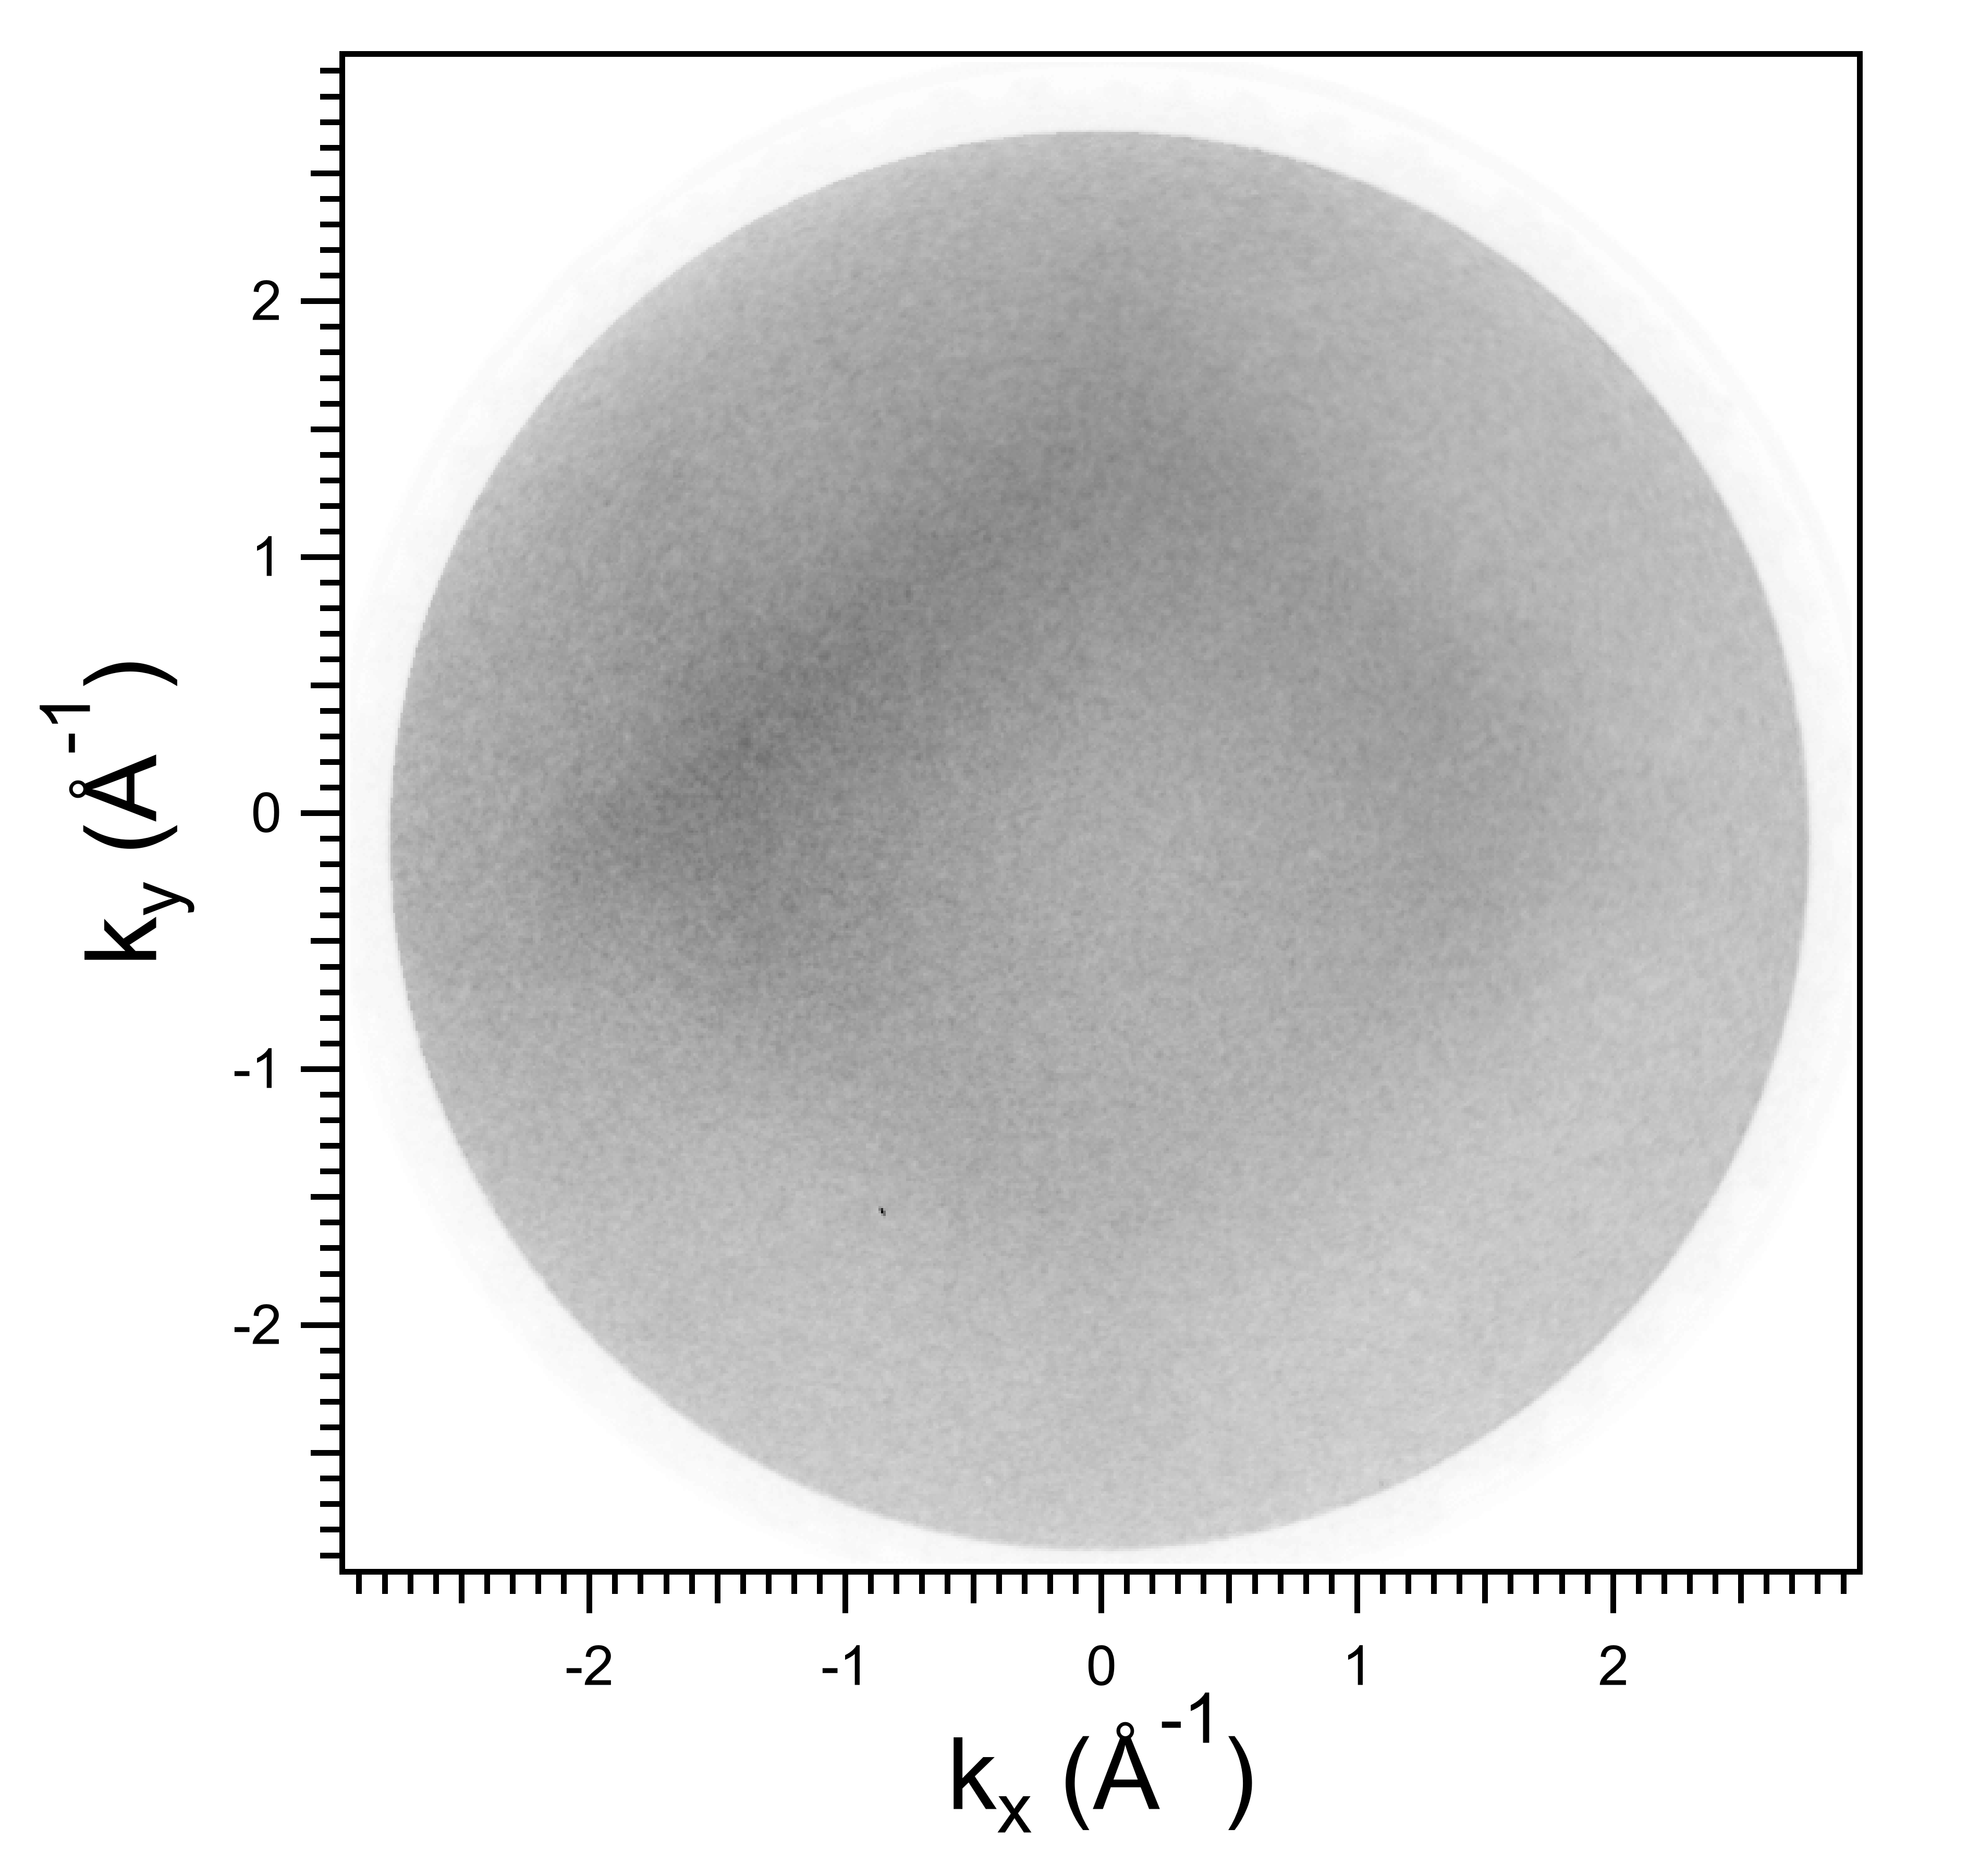
\includegraphics[height=3.7cm]{FeO+5A/FeO_5A_30_95eV.png}
                    \subcaption{\SI{4.55}{\electronvolt}}
                    % Das Bild für eine kinetische Energie von \SI{30.95}{\electronvolt}, also \SI{4.55}{\electronvolt} Bindungsenergie.
                    \label{fig:MOT_FeO+5A_exp_4}
                \end{subfigure}
                \begin{subfigure}[t]{0.48\textwidth}
                    \centering
                    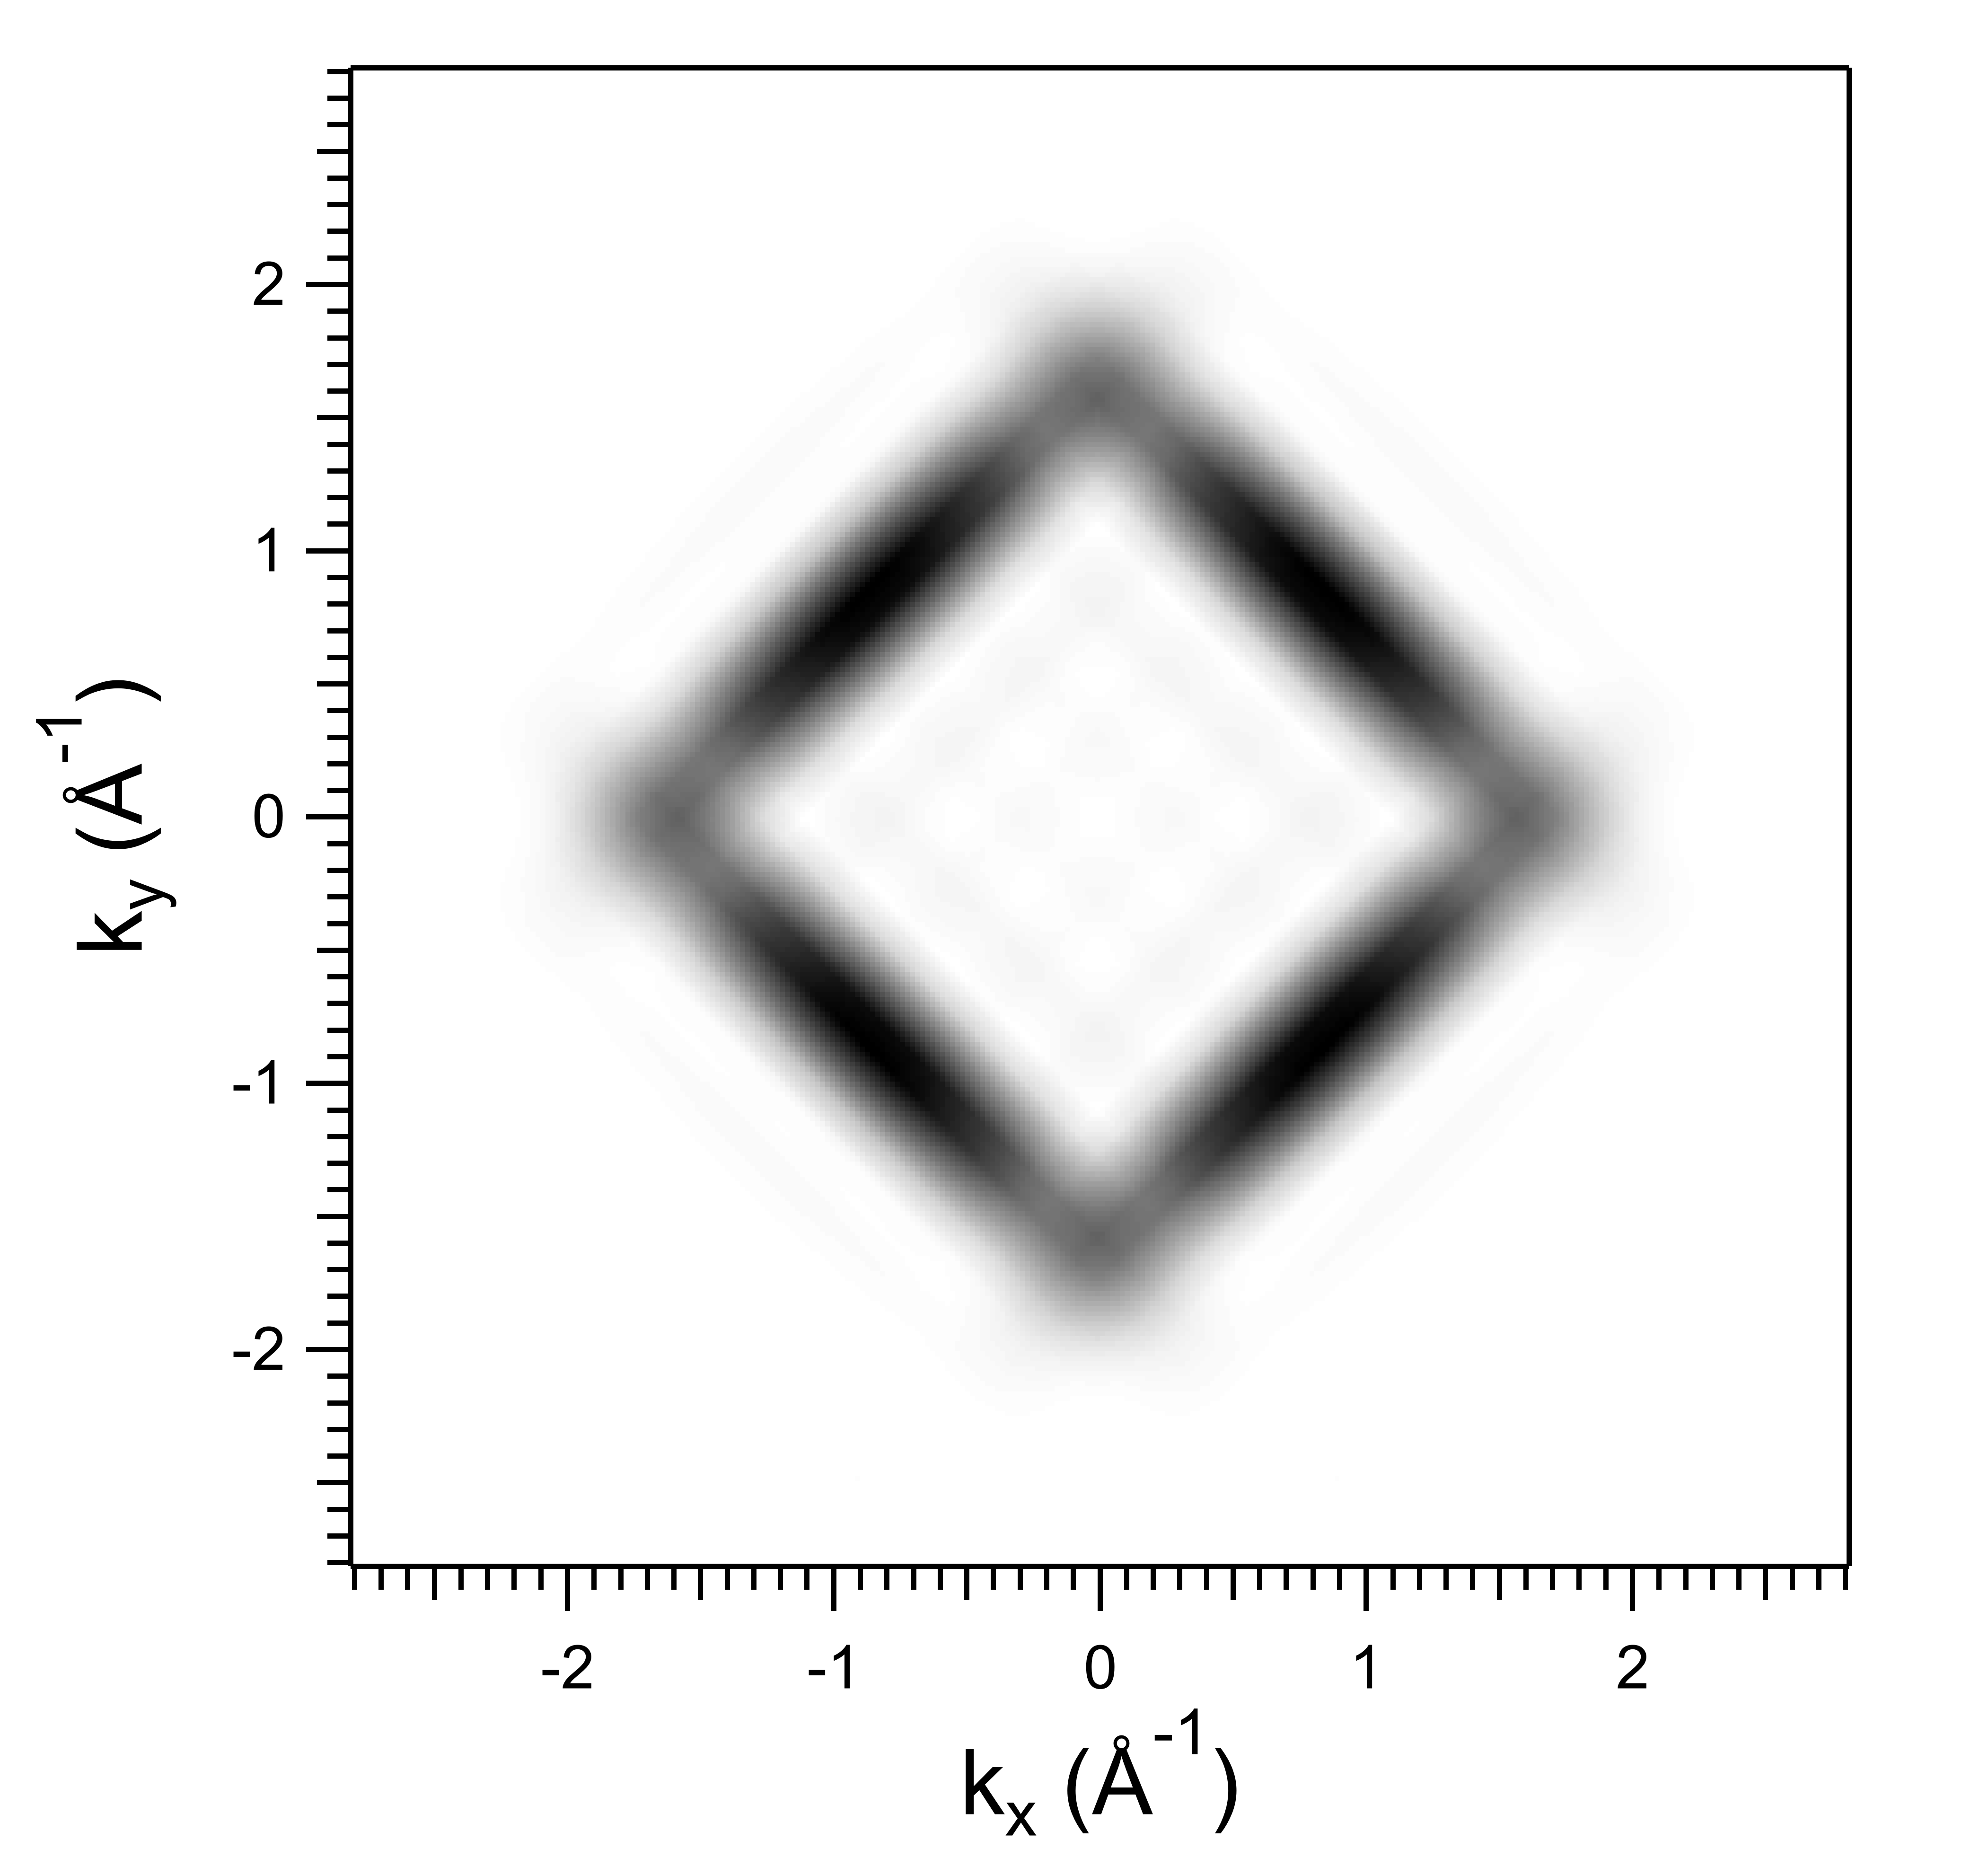
\includegraphics[height=3.7cm]{FeO+5A/MO_HOMO2_RT_RT.png}
                    \subcaption{HOMO-2}
                    % Das HOMO-2 mit Symmetrisierung zweier um \SI{90}{\degree} verdrehten Übergitter.
                    \label{fig:MOT_FeO+5A_theo_4}
                \end{subfigure}
                \begin{subfigure}[t]{\textwidth}
                    \centering
                    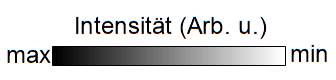
\includegraphics[width=6cm]{Farbskala.png}
                \end{subfigure}
                \caption{Vergleich der gemessenen Intensitätsverteilung für verschiedene Bindungsenergien (links) mit den theoretisch berechneten Intensitätsverteilungen (rechts).
                Die Photonenenergie betrug \SI{40}{\electronvolt} und war p polarisiert.}
                \label{fig:MOT_FeO_5A}
            \end{figure}
            Einige Zuordnungen sind in \autoref{fig:MOT_FeO_5A} zu finden.
            Die theoretisch berechneten Bilder wurden mit Hilfe des Python Programms \textit{kmap.py} erstellt~\cite{brandstetter_kmappy_2021}.
            Anschließend werden die Symmetrien berücksichtigt, in dem zwei um \SI{90}{\degree} zueinander verdrehten Bilder aufsummiert werden.
            Dies rührt von der Substratsymmetrie her, da sich atomare Reihen entlang der Substratachsen ergeben und sich die Moleküle an diesen ausrichten.
            Eine Intensitätsabnahme von oben nach unten bei den gemessenen Bildern ergibt sich aus dem Polarisationfaktor.
            Die Intensität sinkt, wenn der Winkel zwischen einfallenden Photonen von \SI{66}{\degree} zur Oberflächennormalen entlang der negativen $k_\text{y}$-Achse bei $k_\text{x} = \SI[per-mode=reciprocal]{0}{\per\angstrom}$ und den austretenden Elektronen sinkt.

            Das in der Gasphase unbesetzte Molekülorbital LUMO wird durch die Interaktion mit dem Wüstit besetzt.
            Dies lässt sich aus dem Vergleich zwischen dem gemessenen Bild in \autoref{fig:MOT_FeO+5A_exp_1} und der theoretisch berechneten Intensitätsverteilung in \autoref{fig:MOT_FeO+5A_theo_1} erkennen.
            Charakteristisch ist ein quadratähnliche Intensitätsverteilung, welche um \SI{45}{\degree} relativ zur $k_\text{y}$-Achsen gedreht ist.
            Dabei konzentriert sich die Intensität auf das Zentrum der Kanten und es gibt kaum Intensität an den Ecken.
            Zusätzlich ergeben sich Ausläufer an den Ecken welche sich \SI{90}{\degree} zu den Kanten zu steigenden $k$-Werten befinden.
            Auch die Bindungsenergie mit \SI{0.7}{\electronvolt} ist nicht zu groß, sodass sich ein Ladungsaustausch begründen lässt.
            Alle diese Merkmale lassen sich ebenso in der gemessenen Intensitätsbildern wiederfinden, was eine eindeutige Identifizierung zulässt.
            Das HOMO lässt sich bei der Gegenüberstellung der gemessenen (\autoref{fig:MOT_FeO+5A_exp_2}) und den berechneten Intensitäten (\autoref{fig:MOT_FeO+5A_theo_2}) identifizieren.
            Klar erkennbar sind die sternartigen Verläufe. % für $\text{k}_\text{x} = \SI[per-mode=reciprocal]{0}{\per\angstrom}$ und $\text{k}_\text{y} = \pm\SI[per-mode=reciprocal]{1.5}{\per\angstrom}$, sowie $\text{k}_\text{y} = \SI[per-mode=reciprocal]{0}{\per\angstrom}$ und $\text{k}_\text{x} = \pm\SI[per-mode=reciprocal]{1.5}{\per\angstrom}$.
            Bei einer Bindungsenergie von \SI{4.55}{\electronvolt} lässt sich das HOMO-2 aus der theoretischen Berechnung in \autoref{fig:MOT_FeO+5A_theo_4} der gemessenen Intensitätsverteilung in \autoref{fig:MOT_FeO+5A_exp_4} zuordnen.
            In Unterschied zum LUMO befinden sich an den Ecken des Quadrates keine zusätzlichen Merkmale und das Quadrat ist geschlossen.
            Die gemessene Intensitätsverteilung in \autoref{fig:MOT_FeO+5A_exp_3} bei \SI{3.35}{\electronvolt} liegt energetisch zwischen dem identifizieren HOMO und HOMO-2.
            Vermutlich handelt es sich also um das HOMO-1, allerdings zeigt die optische Übereinstimmung zur theoretischen Intensitätsverteilung (\autoref{fig:MOT_FeO+5A_theo_3}) größere Abweichungen.
            So werden Intensitätsmaxima bei $k= \pm\SI[per-mode=reciprocal]{1}{\per\angstrom}$ erwartet, die zu größeren $k$-Werten sternartige Intensitäten aufweisen, die nicht in Richtung Zentrum zeigen.
            An entsprechenden Stellen finden sich zwar erhöhte Intensitäten, allerdings zeigen diese keine sternartigen Intensität, die nach außen laufen.
            Hinzukommend, ist die Intensität welche sich auf den Verbindungslinien zwischen diesen Punkten abzeichnet und nicht in den theoretischen Berechnungen wiedergefunden werden kann.
            Eventuell handelt es sich um eine Überlagerung aus der Beteiligung von HOMO-1 und HOMO-2.
            \begin{figure}
                \centering
                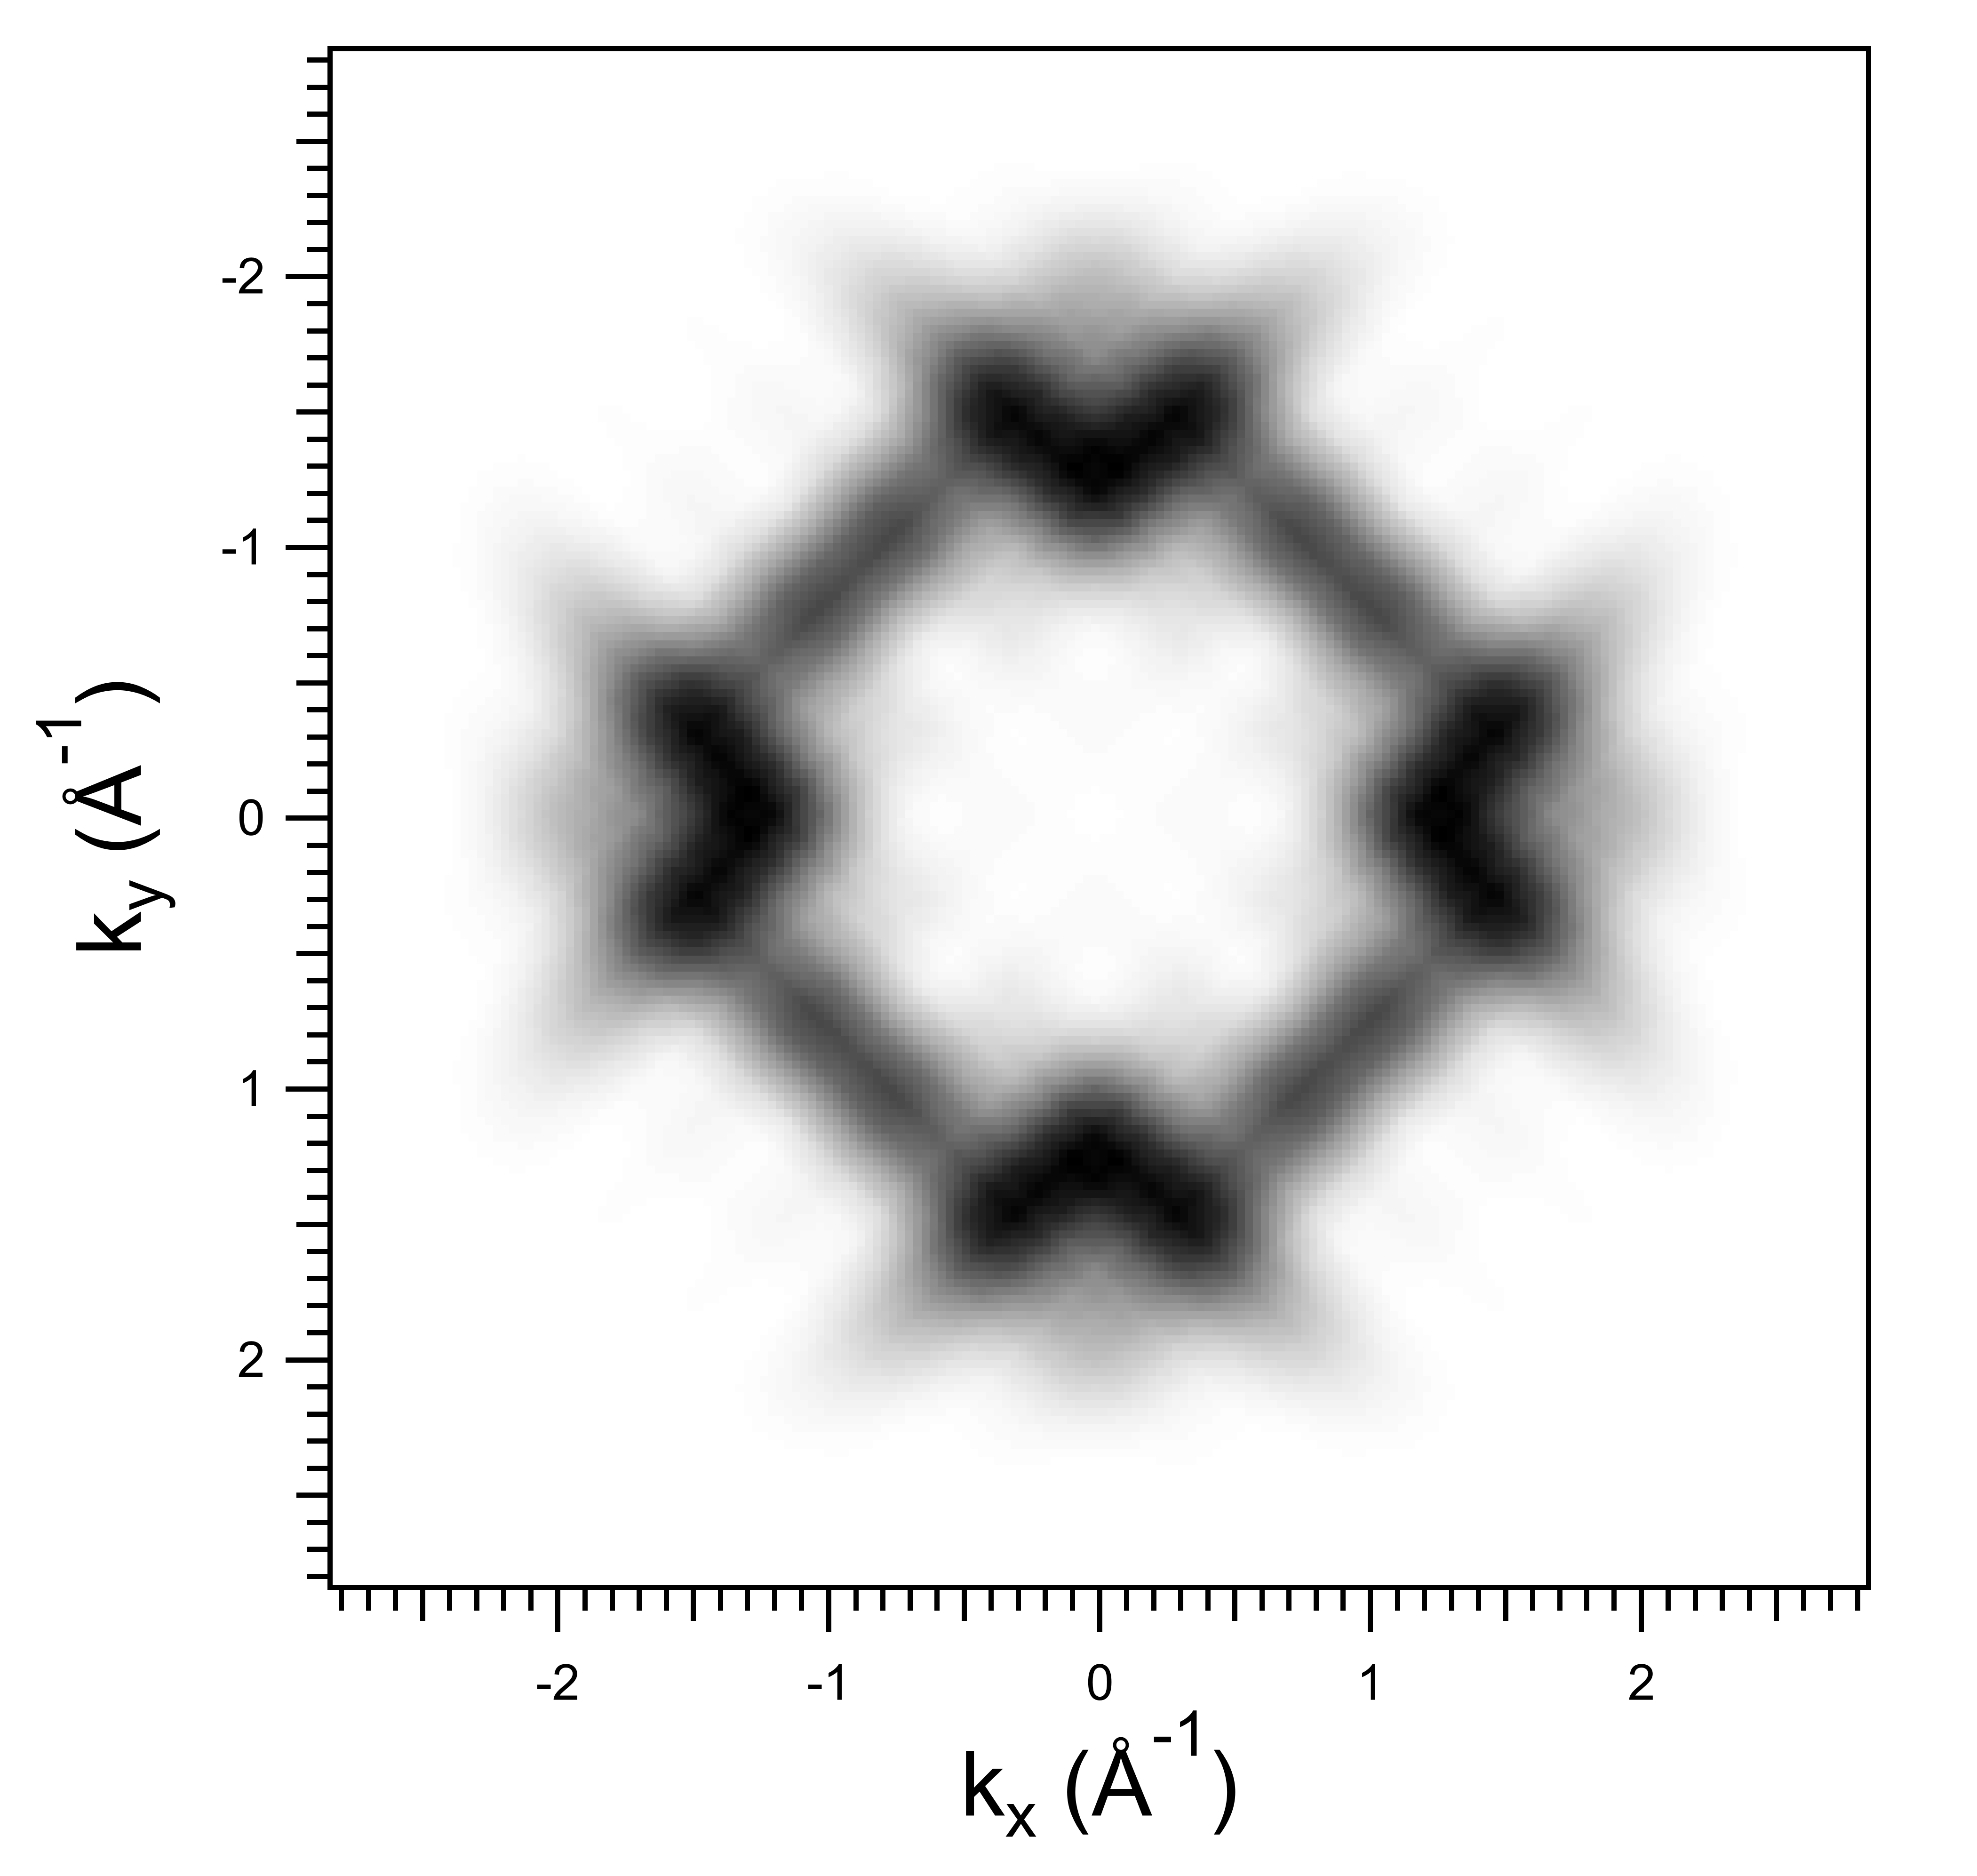
\includegraphics[height=5cm]{HOMO_1_HOMO_2.png}
                \caption{Kalkulierte theoretische Intensitätsverteilung für die überlagerten Molekülorbitale HOMO-1 und HOMO-2.} % bei einer kinetischen Energie von \SI{7.5}{\electronvolt}. Also Bindungsenergie von \SI{3.85}{\electronvolt}.
                \label{fig:MOT_FeO+5A_theo_5}
            \end{figure}
            Dies ist in \autoref{fig:MOT_FeO+5A_theo_5} dargestellt und zeigt eine größere Übereinstimmung als das reine HOMO-1.

            \begin{figure}
                \centering
                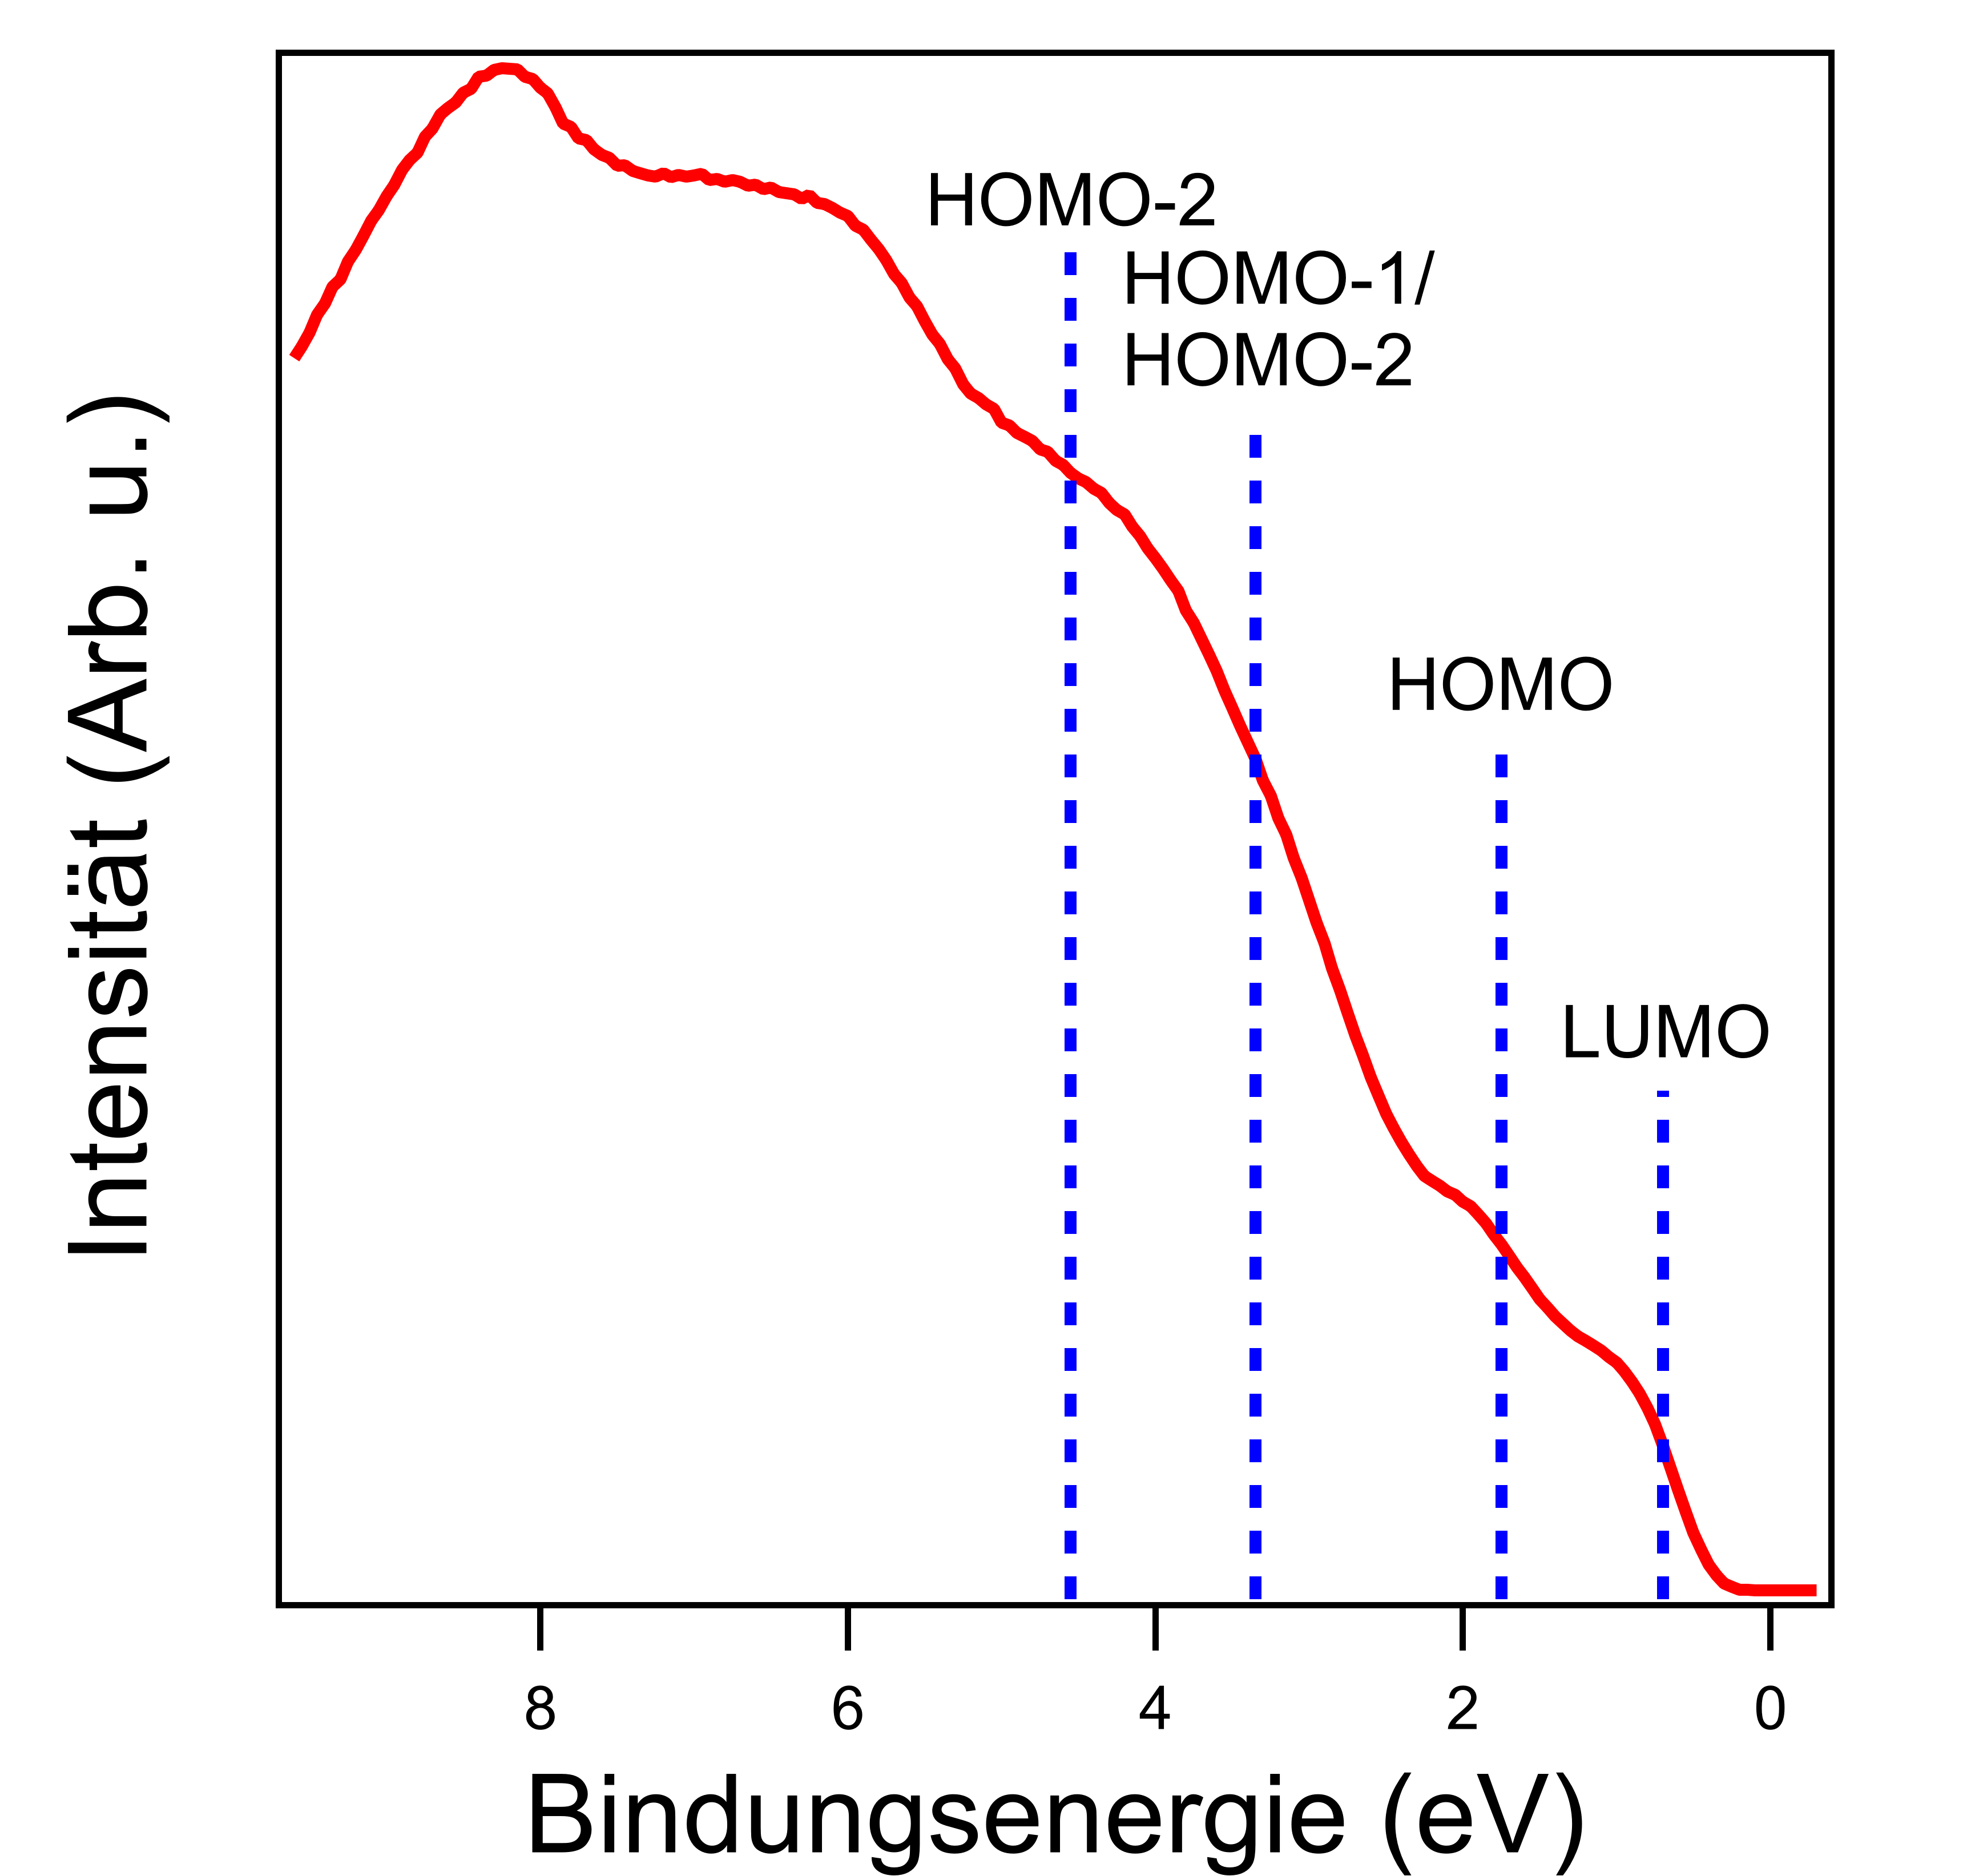
\includegraphics[width=0.5\textwidth]{FeO+5A/VB_FeO_5A.png}
                \caption{Das Valenzbandspektrum der Wüstitoberfläche mit einer Monolage Pentacen bei einer Photonenenergie von \SI{40}{\electronvolt}.}
                \label{fig:EDC_FeO+5A}
            \end{figure}
            Die jeweils identifizieren Merkmale finden sich ebenfalls im winkelintegrierten Spektrum in \autoref{fig:EDC_FeO+5A} wieder.
            An den jeweiligen Positionen befinden sich klar erkennbare Erhebungen.
            % Auch ohne die fehlende Referenzmessung des Substartes lässt sich dies erkennen.

            Es kann davon ausgegangen werden, dass es sich bei der Wechselwirkung um die Chemisorption handelt, denn das LUMO wird besetzt.
            Dies impliziert einen Ladungsaustausch zwischen den Molekülen und dem Substrat.
            Zusätzlich kann angenommen werden, dass sich die Moleküle in eine parallel nebeneinander liegende Anordnung begeben~\cite{IF_13}.
            Dies ergibt sich dabei aus der $\pi-\pi$ Interaktion von größeren Molekülen die aus aromatischen Ringen zusammen gesetzt sind~\cite{IF_13}.
            Aus der Lage der Molekülorbital-Signale relativ zu den Impulsachsen lässt sich schlussfolgern, dass sich die Moleküle entlang der [010]- und [001]-Richtung des Substrates ausrichten.

            Durch das Aufdampfen der Moleküle verschiebt sich die Austrittsarbeit zu \SI{3.51}{\electronvolt}, was kaum einen Unterschied zum reinen Eisenmonooxid darstellt.
            Dabei sorgen Adsorbate normalerweise durch den Push-Back-Effekt zu einer Verringerung der Austrittsarbeit.
            Ihr wirkt aber der Ladungstransfer vom Substrat zum LUMO entgegen was zu einer Vergrößerung der Austrittsarbeit führen würde.
            Diese beiden Effekte scheinen sich hier gegenseitig zu kompensieren.
        % Dieser Ladungsaustausch würde dabei zu einer Erniedrigung der Austrittsarbeit führen.~\cite{Calloni}

        % \begin{figure}
        %     \centering
        %     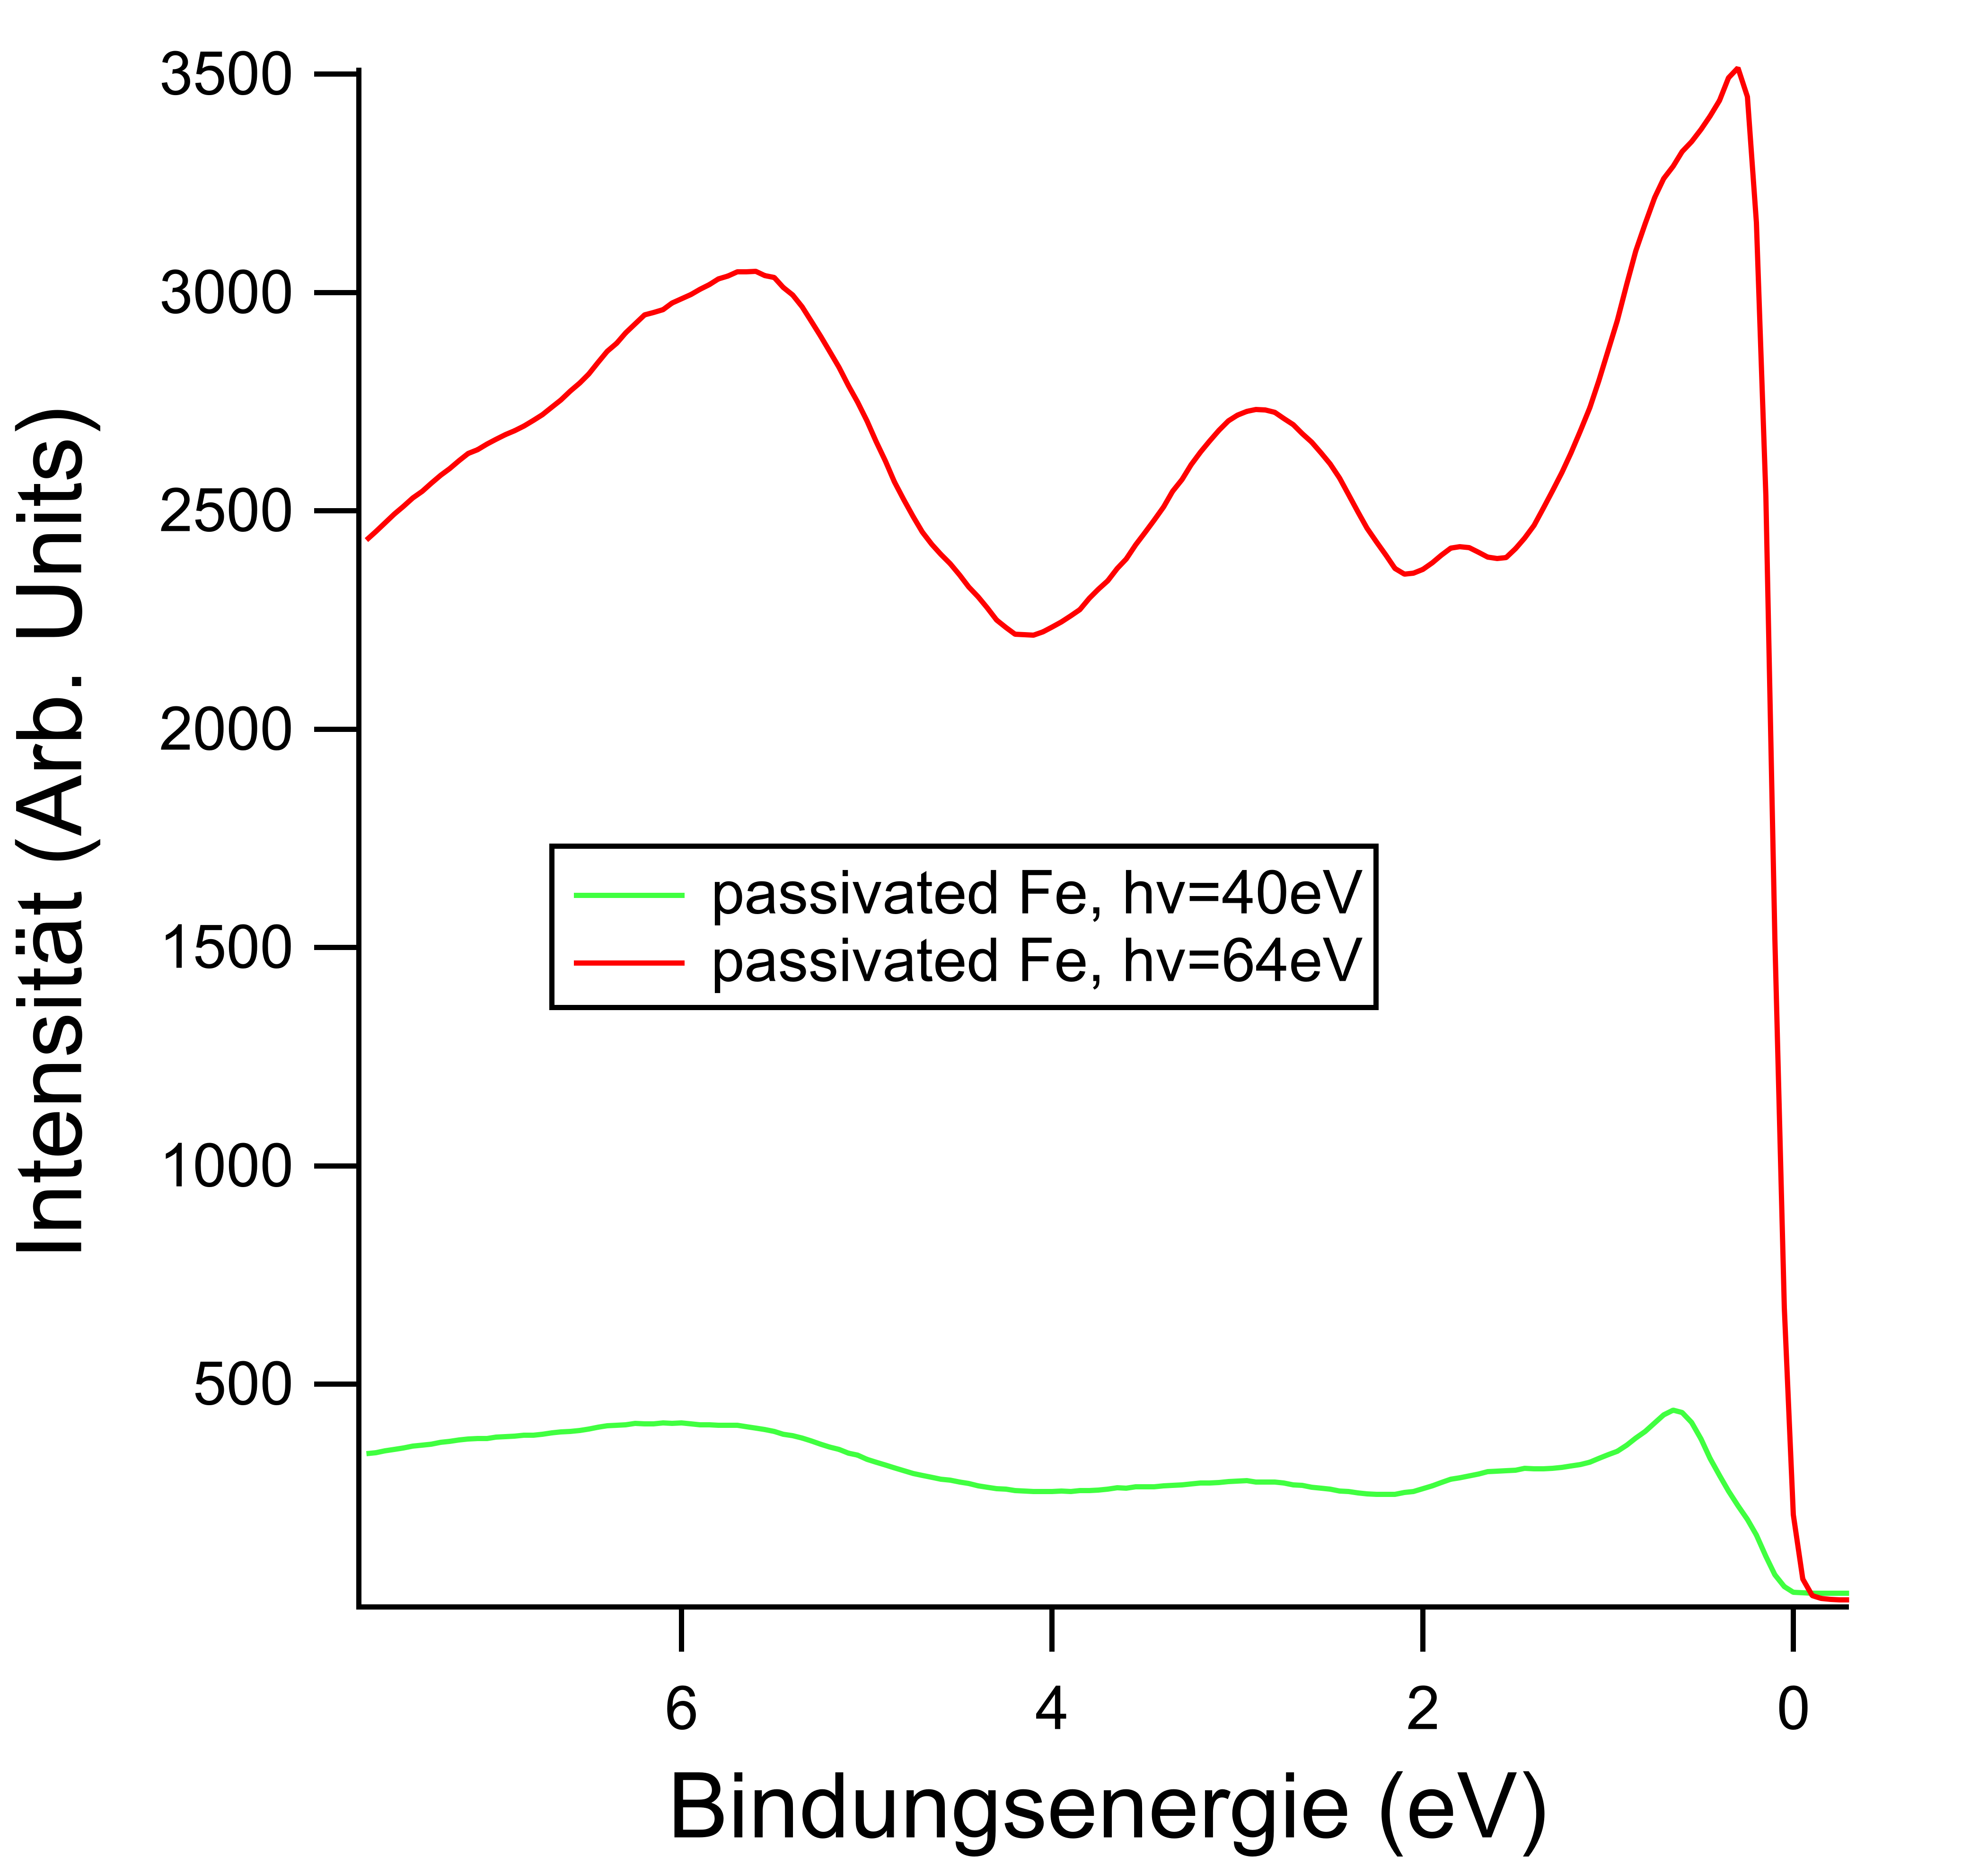
\includegraphics[height=5cm]{pFe/Photonenenergie.png}
        %     \caption{Vergleich des VB-Spektrums bei \SI{64}{\electronvolt} und \SI{40}{\electronvolt} Photonenenergie des passivierten Eisens.}
        %     \label{fig:Photonenenergie}
        % \end{figure}
        % Allerdings ist die eindeutige Zuordnung recht schwierig, da eine Referenzmessung des Substrates bei entsprechnder Photonenenergie nicht aufgenommen wurde.
        % Bei einer anderen Photonenenergie aufgenommene Spektren lassen sich nur schwer als Vergleich heranziehen, da diese deutliche Unterschiede aufweisen können.
        % Als Bespiel sind hier in \autoref{fig:Photonenenergie} zwei Spektren des passivierten Eisens dargestellt bei unterschiedlicher Photonenenergie.
        % Klar zu erkennen ist schon der Unterschied in der Gesamtintensität, was durch den unterschiedlichen Photonenfluss der Beamline für verschiedene Energien zustande kommt.
        % Aber auch bei der Betrachtung der winkelaufgelösten Bilder sind klare Unterschiede hinsichtlich der Merkmale erkennbar.
        % Teilweise zeigen die Bilder bei den gleichen Energien wie die HOMO bis HOMO-2 Orbitale sehr ähnliche Signale wie mit den Molekülen.
  
    % \section{NOTIZEN}
    % \subsection{Datendeutung}
    %     \begin{itemize}
    %         % \item FeO besitzt hingegen nur Fe2+, ist aber recht anfällig weiter zu oxidieren, so dass sich ein Fe3O4 (Fe2+, Fe3+tetra, Fe3+octa) oder Fe2O3 (nur Fe3+) Film bilden kann. 
    %         % \item XAS Messungen wurden duch Multiplikation an Preedge ausgerichtet, dann wurde ein linear Untergrund abgezogen (pre-edge gefittet) und anschließend die Preedge auf Null gesetzt und die Postedge auf 1 (durch Division)
    %         \item Alle Messungen sind Spin integriert, da sonst auch die Einheitszelle größer wäre.
    %         % \item orbital verbreiterung und energie-verschiebung abhängig vom Spin \cite{IF_16}
    %     \end{itemize}

    % \section{Datenformat und Bearbeitung}
    % \begin{itemize}
    %     \item Kreios Vorgehen
    % \end{itemize}
    %     Für die Auswertung der dreidimensionalen Datenwird die Software IGOR Pro~\cite{IGOR} genutzt.
    %     Alle Messungen der winkelaufgelösten Bandstruktur wurden als dreidimensionale Datensätze aufgenommen.
    %     Da die Bilder auf Grund nicht perfekt eingestellter Linsen nicht kreisrund sind, werden die Elipsen angepasst.
    %     Hierfür wird die kleiner der beiden Achsen entlang der Achse gestreckt.
    %     Ferner muss der Polarisationsfaktor unter Beachtung der Substratgeometrie kompensiert werden.
    %     Hierfür werden die Bilder jeweils um \SI{\pm120}{} gedreht und auf das ursprüngliche Bild aufaddiert.
    %     Um die gemessene kinetische Energie in die relevante Bindungsenergie umzurechnen wird bei den integrierten Spektren aus \autoref{sec:EDC} eine Faltung aus \textbf{...} an die Fermikante durchgeführt.
    %     Zusätzlich müssen die gemessenen Bilder von ihren Pixelwerten noch in die entsprechenden Impulswerte umgerechnet werden.
    %     Dies geschieht mit Hilfe der Sekundärelektronen aus dem Spektrum der Austrittsarbeit (niedrige kinetische Energie).
    %     Ihre kinetische Energie kann durch 
    %     \begin{equation}
    %         E_\text{Kin} = \frac{\hbar^2 {k_{||}}^2}{2 m}
    %         \label{eqn:WKF}
    %     \end{equation}
    %     beschrieben werden, wobei $m$ die Elektronenmasse und $k_{||}$ ihr Impuls parallel zur Oberfläche ist.
    %     Die langsamsten Elektronen treten mit einer kinetischen Energie von \SI{0}{\electronvolt} aus der Probe aus und bilden damit den unteren Punkt der Parabel in \autoref{fig:WKF}.
    %     Durch ihren parabolischen Verlauf kann nun bei einer höher liegenden Energie ein Linienprofil genommen werden.
    %     Da sich die Elektronen wie in \autoref{eqn:WKF} verhalten können damit die Pixel in entsprechende Impulswerte umgerechnet werden.